
\documentclass[12pt,twoside]{book}

%%% define a macro \ifpdf para compilação condicional -- PDF ou
%%% DVI/PS.
\usepackage{tikz}

\usepackage[ruled]{algorithm2e}
\renewcommand{\listalgorithmcfname}{Lista de Algoritmos}%
\renewcommand{\algorithmcfname}{Algoritmo}%

%\usepackage{subfigure}
\usepackage{subfloat}

%%% acentuação
\usepackage[latin1]{inputenc}
\usepackage[brazilian,provide=*]{babel}

%%% bibliografia
%\usepackage{chicago}
\usepackage{natbib}

\usepackage{latexsym}


\usepackage{setspace}
\usepackage{mathptm}
\usepackage{latexsym}
\usepackage{amssymb}
\usepackage{xspace}
\usepackage{colortbl}

\usepackage{acronym}
%%% referencias com página \vref
\usepackage[brazil]{varioref}

%%% identa primeiro parágrafo
\usepackage{indentfirst}

%%% figuras um ao lado do outro
\usepackage{subfig}


%%% definir títulos de seção
\usepackage[sf,sl,outermarks]{titlesec}


%%% para tabelas
\usepackage{multirow}

%%% boxes
\usepackage{fancybox}
\usepackage{fancyvrb}
\usepackage{color}

%%% somente na versão PDF

%%% Para inclusão de gráficos
%\usepackage[pdftex]{graphicx}
\usepackage{graphicx}

%%% dimensões do documento
\usepackage[pdftex]{geometry}
  \geometry{a4paper,left=3cm,right=2cm,top=2.0cm,bottom=2cm,twoside}

%%% cria links no arquivo .pdf
%%% comentar as linhas na versão para impressao
\usepackage[pdftex,pdfpagelabels,pagebackref]{hyperref}
%\usepackage{hyperref}


%%% propriedades do arquivo .pdf
\hypersetup{
    pdftitle = {Vis\~ao Computacional para Detec\c{c}\~ao, Segmenta\c{c}\~ao e Organiza\c{c}\~ao Espacial de Parcelas Experimentais de Forrageiras em Imagens Orbitais e de Drone},
    pdfsubject = {Qualifica\c{c}\~ao de Mestrado - Computa\c{c}\~ao Aplicada - UFMS},
    pdfkeywords = {vis\~ao computacional; parcelas experimentais; fenotipagem vegetal; imagens orbitais; drones; detec\c{c}\~ao de objetos},
    pdfauthor = {Raphael Rodrigues}
    }




\hypersetup{colorlinks=true,linkcolor=black,citecolor=black,hypertexnames=false}

%%fonte
\usepackage{bookman}
\usepackage[T1]{fontenc}

%%para os numeros reais
\usepackage{amsfonts}
\usepackage{amsmath}

\DeclareFixedFont{\numberfont}{T1}{phv}{bx}{n}{2cm}

%%% redefine o formato do título



\titleformat{\chapter}[display]
  {\normalfont\Large\sffamily
  }
  {%\titlerule[3pt]%
   \filright
   \rule[32pt]{.7\linewidth}{4pt}
   \hspace{-11pt}
   \shadowbox{
   \begin{minipage}{.18\linewidth}
     \begin{center}
       \textsc{\Large\chaptertitlename}\\
       \vspace{1ex}
       {\numberfont\color[gray]{0.5} \thechapter}\\
       \vspace{1ex}
     \end{center}
   \end{minipage}}
  }
  {0pt}
  {\filcenter
   \Huge
   }
  [\hfill\rule{.8\textwidth}{0.5pt}\\
     \vskip-1.8ex\hfill\rule{.7\textwidth}{3pt}]


%%% macro para destacar a(s) primeira(s) letra do texto
%%% é necessário ter a fonte courier instalada
%
%  um texto do tipo:
%
%  \begin{document}
%    \versal{IN} THE beginning God created the heaven and the earth.  Now the
%    earth was unformed and void, and darkness was upon the face of the
%    deep; and the spirit of God hovered over the face of the waters.
%  \end{document}
%
%  irá produzir algo como:
%
%  I I\  I THE beginning God  created the heaven and  the earth.
%  I I \ I Now the earth was unformed and void, and darkness was
%  I I  \I upon the face of the deep; and the spirit of God hov-
%  ered over the face of the waters.

%\font\largefont= pzcmi scaled 6500

\newcommand{\versal}[1]{{\noindent
    \setbox0\hbox{\largefont #1 }%
    \count0=\ht0                   % height of versal
    \count1=\baselineskip          % baselineskip
    \divide\count0 by \count1      % versal height/baselineskip
    \dimen1 = \count0\baselineskip % distance to drop versal
    \advance\count0 by 1\relax     % no of indented lines
    \dimen0=\wd0                   % width of versal
    \global\hangindent\dimen0      % set indentation distance
    \global\hangafter-\count0      % set no of indented lines
    \hskip-\dimen0\setbox0\hbox to\dimen0{\raise-\dimen1\box0\hss}%
    \dp0=0in\ht0=0in\box0}}
% Backref com colocação de "Citado na página..."
\renewcommand*{\backref}[1]{}
\renewcommand*{\backrefalt}[4]{
   \ifcase #1
       Não citado no texto.
   \or
       Citado na página~#2.
   \else
       Citado nas páginas #2.
   \fi
}

\renewcommand{\backreftwosep}{ e~}
\renewcommand{\backreflastsep}{, e~}


\usepackage{pgf}
\usepackage{baseboxes}
\usepackage{basecolor}

% Este documento (qualificacao) nao reaproveita nenhuma das macros
% definidas no macros.tex do modelo (elas eram especificas da tese de
% Edson Takashi Matsubara: \lexrank, \progroc, \cotraining etc.).
%
% Uma unica macro auxiliar e definida abaixo: o modelo (tese.pdf) nao
% contem nenhuma figura, logo nao define nenhum padrao de "Fonte:"
% sob as imagens. Como todas as 14 figuras do documento original
% trazem essa linha (ex.: "Fonte: Elaborado pelo autor (2026)."),
% \fonte reproduz esse conteudo de forma consistente, fora do texto
% do \caption (para nao poluir a Lista de Figuras).
\newcommand{\fonte}[1]{{\centering\footnotesize Fonte: #1\par}}


\begin{document}

\pagestyle{empty}
\pagenumbering{roman}


\newcommand{\titulo}{Vis\~ao Computacional para Detec\c{c}\~ao, Segmenta\c{c}\~ao e Organiza\c{c}\~ao Espacial de Parcelas Experimentais de Forrageiras em Imagens Orbitais e de Drone}
  

\begin{titlepage}

\ \vfill

\begin{center}
\begin{minipage}[c]{12cm}
\begin{center}
\hrulefill\\
\vspace{.5cm} {\Large \titulo}\\
\vspace{1.3cm}

\textbf{\it Raphael Rodrigues Gon\c{c}alves}\\
\vspace{.5cm}
\hrulefill\\
\end{center}
\end{minipage}
\end{center}

\vfill

\cleardoublepage

\vspace*{2cm}
\begin{center}
{\huge\sf \titulo}

\vspace*{2cm}

{\it Raphael Rodrigues Gon\c{c}alves}

\vspace*{2cm}


\textbf{UFMS - Universidade Federal de Mato Grosso do Sul}

\vspace*{1cm}

\textbf{T\'itulo provis\'orio:} \titulo

\vspace*{1cm}

\textbf{Programa de P\'os-Gradua\c{c}\~ao:} \\
Mestrado em Computa\c{c}\~ao Aplicada

\vspace*{1cm}


{\bf Orientador:}  {\it Prof. Dr. Edson Takashi Matsubara}

\end{center}


\cleardoublepage



\end{titlepage}


\pagestyle{plain}


\onehalfspacing

\chapter*{Agradecimentos}

Primeiramente, agrade\c{c}o a Deus, pela vida, pelas oportunidades e pela sabedoria concedida ao longo desta caminhada. \`{A} minha fam\'ilia e aos meus amigos, pelo apoio, pela compreens\~ao e pelo incentivo em todos os momentos deste processo. Em especial, agrade\c{c}o aos meus maiores incentivadores, minha esposa, Nayara Ortiz Isume, meus amigos, Rodrigo Luiz Chaves, Maykon Kazuhiro meu parceiro de equipe, que estiveram ao meu lado e contribu\'iram para que eu seguisse em frente, mesmo diante dos desafios. Aos meus colegas de trabalho, agrade\c{c}o pela compreens\~ao, pelo apoio e, sobretudo, pela paci\^encia ao longo deste per\'iodo, especialmente nos momentos em que foi necess\'ario conciliar as responsabilidades profissionais com as exig\^encias da vida acad\^emica. De maneira especial, registro minha gratid\~ao aos meus chefes e, com orgulho, amigos, Paulo Cezar, superintendente da Sitec, e Diego Janu\'ario, coordenador na Secretaria de Estado de Educa\c{c}\~ao de Mato Grosso do Sul, pela compreens\~ao, pelo apoio e pela confian\c{c}a durante esta caminhada.

Aos professores da Faculdade de Computa\c{c}\~ao (FACOM), por todo o conhecimento compartilhado ao longo desta trajet\'oria, ao meu orientador, Prof. Dr. Edson Takashi Matsubara, pela orienta\c{c}\~ao, confian\c{c}a, disponibilidade e pelas contribui\c{c}\~oes fundamentais para o desenvolvimento deste trabalho.

Aos demais integrantes da equipe do projeto, Jo\~ao e Geazi, pelo trabalho conjunto, pelas discuss\~oes e pelas contribui\c{c}\~oes ao longo do desenvolvimento da pesquisa.

Agrade\c{c}o tamb\'em \`{a}s pessoas que, de diferentes formas, contribu\'iram para a constru\c{c}\~ao deste projeto: ao meu colega Leonardo Crivellaro, ao Prof. Wesley Nunes Gon\c{c}alves, da Universidade Federal de Mato Grosso do Sul, e aos colaboradores da Embrapa, Camilo Carromeu, Mateus Figueiredo Santos e Celina Ragalzi.

Por fim, a todos que fizeram parte, direta ou indiretamente, desta caminhada e contribu\'iram para que este trabalho se tornasse poss\'ivel, registro minha sincera gratid\~ao.

\cleardoublepage
\chapter*{Resumo}

A identifica\c{c}\~ao e a organiza\c{c}\~ao espacial de parcelas experimentais em imagens orbitais e de drone constituem um desafio para a an\'alise automatizada de ensaios agr\'icolas, principalmente quando a densidade, a orienta\c{c}\~ao e a variabilidade visual das parcelas afetam o desempenho dos detectores. Esta pesquisa tem como objetivo investigar m\'etodos de vis\~ao computacional para detectar, localizar e organizar parcelas experimentais de forrageiras e avaliar como a composi\c{c}\~ao do conjunto de treinamento influencia a capacidade de generaliza\c{c}\~ao do detector. A metodologia compreende a constru\c{c}\~ao e a reorganiza\c{c}\~ao progressiva dos conjuntos de dados, o treinamento e a avalia\c{c}\~ao de modelos para segmenta\c{c}\~ao e detec\c{c}\~ao de parcelas, al\'em da investiga\c{c}\~ao de abordagens auxiliares para localiza\c{c}\~ao, classifica\c{c}\~ao da dificuldade das imagens e associa\c{c}\~ao espacial entre parcelas. As avalia\c{c}\~oes realizadas evidenciaram diferen\c{c}as de desempenho entre as representa\c{c}\~oes investigadas, com destaque das caixas delimitadoras orientadas em parte das m\'etricas, sem que essas diferen\c{c}as possam ser atribu\'idas exclusivamente ao tipo de representa\c{c}\~ao. Tamb\'em foi aplicado um procedimento de associa\c{c}\~ao geom\'etrica das parcelas entre imagens de um mesmo campo, que atribuiu identificador a 90,77\% dos objetos, sem que a corre\c{c}\~ao desses identificadores tenha sido medida; permanecem ainda limita\c{c}\~oes relacionadas \`{a} independ\^encia entre as imagens de treinamento e de teste. Como contribui\c{c}\~ao da pesquisa, ser\'a investigada uma estrat\'egia de sele\c{c}\~ao das imagens de treinamento orientada por um crit\'erio quantitativo de instabilidade das predi\c{c}\~oes, estimado em imagens n\~ao utilizadas no treinamento, e comparada ao conjunto completo, a subconjuntos aleat\'orios de mesmo tamanho e ao limiar hist\'orico de F1-Score de 0,97.

\textbf{Palavras-chave:} vis\~ao computacional; parcelas experimentais; fenotipagem vegetal; imagens orbitais; drones; detec\c{c}\~ao de objetos.

\chapter*{Abstract}

The identification and spatial organization of experimental plots in satellite and drone imagery constitute a challenge for the automated analysis of agricultural trials, particularly when plot density, orientation, and visual variability affect detector performance. This research aims to investigate computer vision methods for detecting, locating, and organizing experimental forage plots, and to assess how the composition of the training set influences the detector's generalization capability. The methodology comprises the construction and progressive reorganization of the datasets, the training and evaluation of models for plot segmentation and detection, as well as the investigation of auxiliary approaches for localization, image difficulty classification, and spatial association between plots. The evaluations carried out revealed performance differences among the representations investigated, with oriented bounding boxes standing out in some of the metrics, although these differences cannot be attributed exclusively to the type of representation. A procedure for the geometric association of plots across images of the same field was also applied, which assigned an identifier to 90.77\% of the objects, without the correctness of these identifiers having been measured; limitations remain regarding the independence between the training and test images. As a contribution of this research, a strategy for selecting training images guided by a quantitative criterion of prediction instability, estimated on images not used in training, will be investigated and compared against the full set, random subsets of the same size, and the historical F1-Score threshold of 0.97.

\textbf{Keywords:} computer vision; experimental plots; plant phenotyping; satellite imagery; drones; object detection.

\cleardoublepage
\tableofcontents
\addcontentsline{toc}{section}{Sum\'ario}
\cleardoublepage

\listoffigures
\addcontentsline{toc}{section}{Lista de Figuras}
\cleardoublepage

\listoftables
\addcontentsline{toc}{section}{Lista de Tabelas}
\cleardoublepage




\pagenumbering{arabic}



\chapter{Introdu\c{c}\~ao}
\label{cap:introducao}

A experimenta\c{c}\~ao \`a campo ocupa papel fundamental nos programas de melhoramento vegetal, pois permite avaliar materiais gen\'eticos sob condi\c{c}\~oes reais de cultivo. Esse processo depende da observa\c{c}\~ao sistem\'atica de caracter\'isticas fenot\'ipicas relacionadas ao desenvolvimento, \`a produtividade e \`a adapta\c{c}\~ao das plantas. \`A medida que aumenta o n\'umero de gen\'otipos, \'areas e momentos de avalia\c{c}\~ao, cresce tamb\'em a demanda por m\'etodos capazes de ampliar a aquisi\c{c}\~ao e o processamento das informa\c{c}\~oes experimentais. Esse cen\'ario tem impulsionado estrat\'egias de fenotipagem de alto rendimento, nas quais sensores e m\'etodos computacionais s\~ao empregados para reduzir a depend\^encia de avalia\c{c}\~oes exclusivamente manuais \citep{araus2014}.

As imagens de sensoriamento remoto constituem uma das fontes utilizadas nesse processo. A literatura agr\'icola contempla tanto aquisi\c{c}\~oes orbitais quanto imagens obtidas por plataformas a\'ereas de baixa altitude. Em experimentos com forrageiras tropicais, estudos realizados em colabora\c{c}\~ao com a \textbf{Embrapa Gado de Corte} (Centro Nacional de Pesquisa de Gado de Corte) e a \textbf{UFMS - Universidade Federal de Mato Grosso do Sul} investigam imagens obtidas por VANT (Ve\'iculo A\'ereo N\~ao Tripulado) para estimativa de biomassa e rendimento de mat\'eria seca \citep{castro2020,oliveira2021}. Esses trabalhos caracterizam o dom\'inio de aplica\c{c}\~ao, e os dados desta qualifica\c{c}\~ao re\'unem imagens orbitais e ortomosaicos (mapa de alta resolu\c{c}\~ao formado pela uni\~ao de v\'arias fotografias a\'ereas) obtidos por drones.

No ensaio agron\^omico, entretanto, n\~ao basta reconhecer vegeta\c{c}\~ao na imagem. Os materiais avaliados s\~ao distribu\'idos em parcelas que ocupam posi\c{c}\~oes previamente definidas no delineamento experimental. Para que uma informa\c{c}\~ao extra\'ida da imagem possa ser relacionada ao gen\'otipo, tratamento ou unidade correspondente, \'e necess\'ario localizar e delimitar cada parcela e estabelecer sua rela\c{c}\~ao com o croqui, que representa a disposi\c{c}\~ao planejada das unidades experimentais. A identifica\c{c}\~ao das parcelas constitui, portanto, uma etapa anterior \`a extra\c{c}\~ao e \`a compara\c{c}\~ao de caracter\'isticas fenot\'ipicas.

Parte desse trabalho pode ser realizada manualmente ou com o apoio de ferramentas voltadas \`a manipula\c{c}\~ao de imagens georreferenciadas. O \textbf{FIELDimageR}, por exemplo, disponibiliza recursos para gera\c{c}\~ao e ajuste de grades sobre ortomosaicos destinados \`a an\'alise de experimentos agr\'icolas \citep{matias2020}. Ainda assim, opera\c{c}\~oes de posicionamento, dimensionamento e corre\c{c}\~ao das regi\~oes de interesse podem exigir interven\c{c}\~ao humana, principalmente quando diferentes \'areas ou per\'iodos precisam ser processados.

A localiza\c{c}\~ao autom\'atica de parcelas experimentais tem sido investigada por diferentes estrat\'egias, que v\~ao da segmenta\c{c}\~ao semiautomatizada a partir de imagens a\'ereas \citep{robb2020} ao ajuste de uma grade associada ao delineamento \citep{khan2019,mardanisamani2021}, ao acoplamento entre redes convolucionais e processamento geom\'etrico \citep{han2024} e \`a segmenta\c{c}\~ao orientada para parcelas rotacionadas \citep{zhang2025}. Em conjunto, esses trabalhos mostram que a extra\c{c}\~ao de parcelas depende n\~ao apenas da evid\^encia visual, mas tamb\'em da geometria e da disposi\c{c}\~ao espacial das unidades experimentais; a rela\c{c}\~ao entre eles e o procedimento adotado nesta pesquisa \'e retomada na Se\c{c}\~ao~\ref{sec:relacao-literatura}.

Outro aspecto relevante \'e a composi\c{c}\~ao dos dados empregados no treinamento dos modelos. Trabalhos de detec\c{c}\~ao supervisionada que priorizam exemplos dif\'iceis, organizam as amostras por dificuldade ou selecionam subconjuntos representativos indicam que as amostras de treinamento n\~ao precisam ser tratadas como igualmente informativas e que sua sele\c{c}\~ao pode ser investigada como parte do processo de aprendizagem \citep{shrivastava2016,wang2018,lee2024}. Essa literatura \'e detalhada na Se\c{c}\~ao~\ref{sec:generalizacao-dependencia}.

\'E nesse contexto que se insere o trabalho, desenvolvido no \^ambito do projeto \textbf{PhenoSight}, conduzido de forma colaborativa com a Embrapa Gado de Corte, sob orienta\c{c}\~ao do professor Dr. Edson Takashi Matsubara. O objetivo deste projeto \'e criar ferramentas de vis\~ao computacional que possam identificar, delimitar, quantificar, posicionar e arranjar \'areas de cultivo de forrageiras para pesquisa. Para tanto, foram empregadas imagens provenientes de sat\'elites e de drones, com subsequente avalia\c{c}\~ao da conex\~ao entre as informa\c{c}\~oes usadas no aprendizado das ferramentas, a efic\'acia da detec\c{c}\~ao e a organiza\c{c}\~ao geogr\'afica das parcelas.

\begin{figure}[htb]
  \centering
  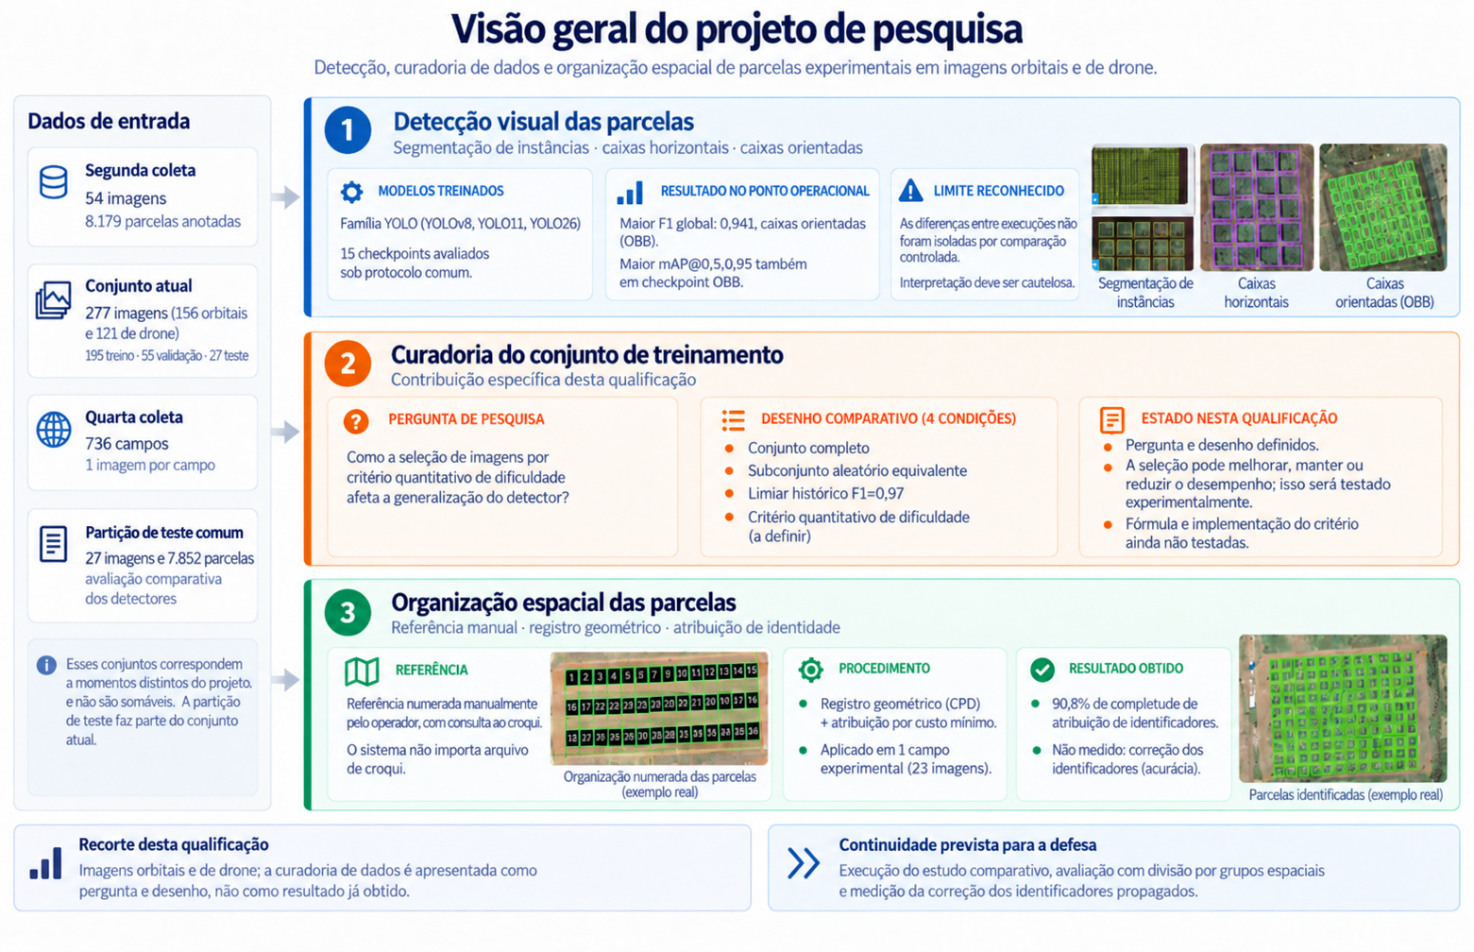
\includegraphics[width=0.95\textwidth]{figuras/figura01.png}
  \caption{Vis\~ao geral das principais frentes metodol\'ogicas do projeto de pesquisa.}
  \label{fig:visao-geral-frentes}
  \fonte{Elaborado pelo autor (2026).}
\end{figure}

O acervo anotado foi ampliado ao longo do projeto. A primeira coleta, foi de 35 imagens e 3.444 parcelas, mas n\~ao catalogada, j\'a a segunda coleta reuniu 54 imagens e 8.179 parcelas anotadas em formato poligonal; o conjunto usado nos experimentos mais recentes t\^em 277 imagens, orbitais e de drone, com 51.245 parcelas divididas entre treinamento, valida\c{c}\~ao e teste; e a coleta em andamento, com imagens orbitais de 1.045 campos experimentais e novos ortomosaicos obtidos por drone, que deve ultrapassar mais de 1.200 imagens de campo. Esses n\'umeros correspondem a momentos distintos do projeto e n\~ao s\~ao som\'aveis. A composi\c{c}\~ao e o uso de cada conjunto s\~ao detalhados na se\c{c}\~ao ``Metodologia''.

Ao longo desse desenvolvimento, foram investigadas diferentes formas de representar e localizar as parcelas, incluindo segmenta\c{c}\~ao de inst\^ancias, detec\c{c}\~ao por caixas delimitadoras horizontais, detec\c{c}\~ao por caixas delimitadoras orientadas e uma abordagem alternativa baseada em mapas de confian\c{c}a. Tamb\'em foi estudado, um classificador auxiliar, relacionado \`a dificuldade das imagens e procedimentos de associa\c{c}\~ao espacial destinados a preservar a identifica\c{c}\~ao das parcelas entre imagens de uma mesma \'area \`a campo. Essas frentes permitiram avan\c{c}ar na identifica\c{c}\~ao e na organiza\c{c}\~ao das parcelas visualmente detect\'aveis, embora situa\c{c}\~oes em que a estrutura experimental prev\^e uma posi\c{c}\~ao sem detec\c{c}\~ao correspondente ainda exijam tratamento espec\'ifico.

\begin{figure}[htb]
  \centering
  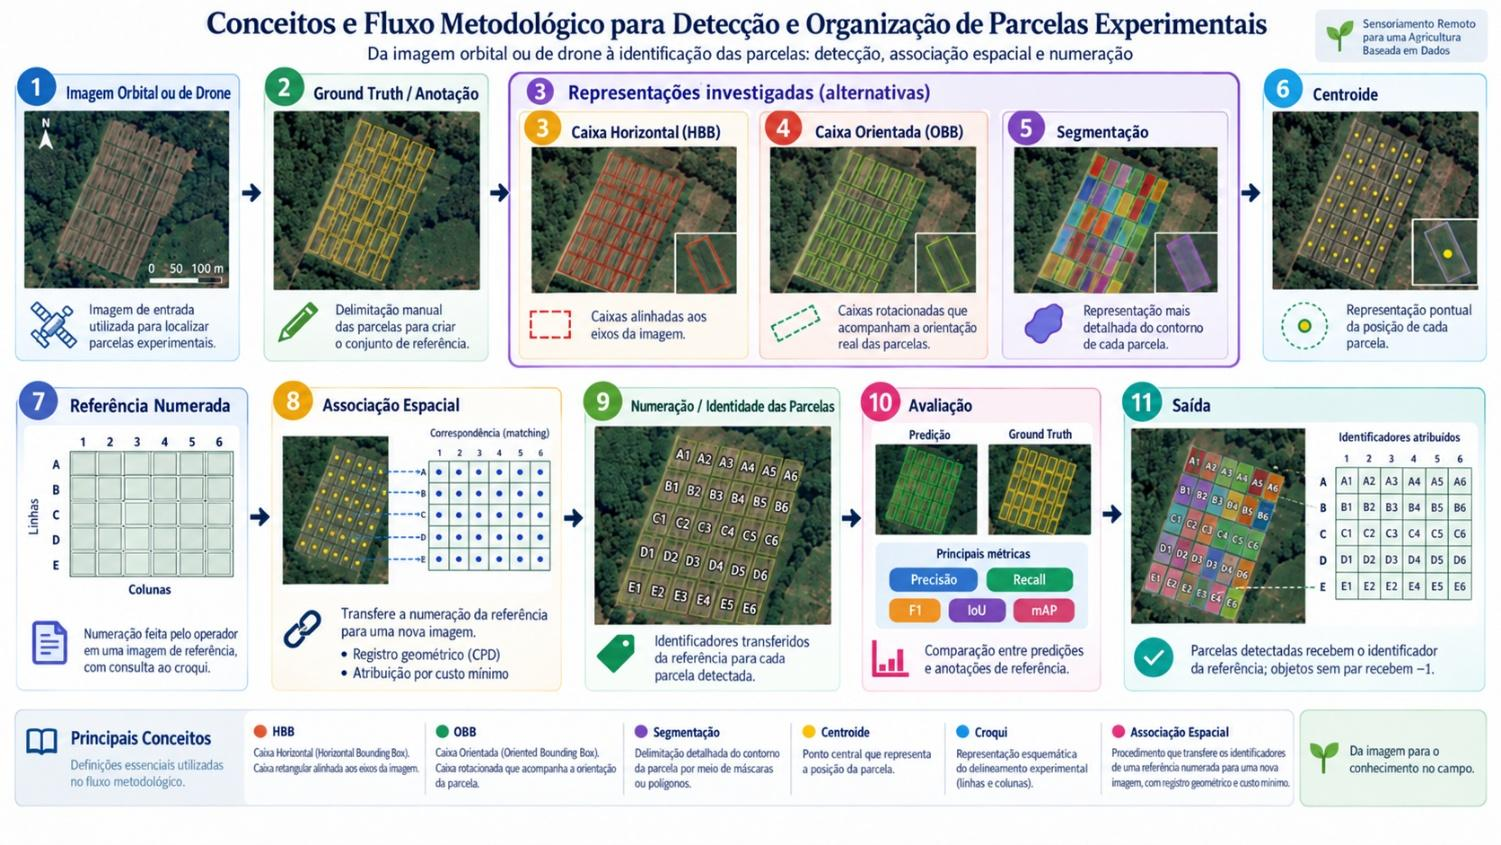
\includegraphics[width=0.95\textwidth]{figuras/figura02.jpg}
  \caption{Conceitos e fluxo metodol\'ogico para detec\c{c}\~ao e organiza\c{c}\~ao de parcelas experimentais em imagens orbitais e de drone.}
  \label{fig:conceitos-fluxo}
  \fonte{Elaborado pelo autor (2026).}
\end{figure}

A evolu\c{c}\~ao dos experimentos revelou tamb\'em uma quest\~ao metodol\'ogica relacionada \`a pr\'opria composi\c{c}\~ao do conjunto de treinamento. Essa composi\c{c}\~ao n\~ao foi originalmente tratada como uma vari\'avel experimental controlada. Em 2025, as imagens receberam manualmente n\'iveis de dificuldade, e as de n\'ivel mais alto foram replicadas no treinamento de parte dos modelos, sem compara\c{c}\~ao com um treinamento n\~ao ponderado nas mesmas condi\c{c}\~oes. Posteriormente, um limite hist\'orico da m\'etrica F1-Score igual a 0,97, por indica\c{c}\~ao do professor, foi empregado para classificar as imagens de acordo com a complexidade exibida ao detector, com o prop\'osito de criar os r\'otulos para um classificador secund\'ario; tal m\'etodo n\~ao foi planejado nem examinado como t\'atica para escolher as imagens usadas no treino do detector. Da mesma forma, foram encontradas imagens da mesma regi\~ao em divis\~oes distintas do conjunto de dados, o que sublinha a import\^ancia de verificar a generaliza\c{c}\~ao em grupos que n\~ao estiveram envolvidos no treino.

Um ponto importante levantado nesta pesquisa, \'e de como a sele\c{c}\~ao das imagens de treinamento por um crit\'erio quantitativo de instabilidade das predi\c{c}\~oes, estimado fora da amostra, afeta na generaliza\c{c}\~ao do detector de parcelas, em compara\c{c}\~ao com o conjunto completo, com subconjuntos aleat\'orios de mesmo tamanho e com o limiar hist\'orico j\'a mencionado. Com isso, surge a hip\'otese de pesquisa deste trabalho, com um conjunto de dados selecionado atrav\'es deste m\'etodo resultando em um detector com melhor capacidade de generaliza\c{c}\~ao em compara\c{c}\~ao com aqueles criados a partir de conjuntos de dados aleat\'orios de tamanho similar. A an\'alise com o conjunto de dados integral serve para mensurar o impacto da diminui\c{c}\~ao do volume de imagens, sem, no entanto, garantir a preserva\c{c}\~ao do desempenho; a escolha poder\'a tanto aprimorar, manter quanto prejudicar o desempenho, e isso ser\'a verificado atrav\'es de experimentos.

Dito isso, podemos descrever como objetivo geral deste projeto:

Investigar e avaliar m\'etodos de vis\~ao computacional para identificar, localizar e organizar parcelas experimentais de forrageiras em imagens orbitais e de drone, com \^enfase na an\'alise do efeito da composi\c{c}\~ao do conjunto de treinamento sobre a generaliza\c{c}\~ao do detector. Para isso, a trajet\'oria j\'a desenvolvida de detec\c{c}\~ao, segmenta\c{c}\~ao e representa\c{c}\~ao espacial ser\'a articulada a um estudo comparativo controlado de diferentes estrat\'egias de composi\c{c}\~ao dos dados.

Ser\~ao comparados o conjunto completo de imagens, subconjuntos aleat\'orios de mesmo tamanho, como j\'a mencionado, com um limiar hist\'orico, e um crit\'erio de instabilidade das predi\c{c}\~oes adaptado do Variance-based Prediction Score \citep{yagi2025}, por ser similar, sendo um aprendizado supervisionado.

A relev\^ancia dessa investiga\c{c}\~ao, est\'a em tratar a composi\c{c}\~ao do conjunto de treinamento como parte expl\'icita do problema de detec\c{c}\~ao, em vez de restringir a an\'alise \`a escolha da arquitetura ou ao valor final de uma m\'etrica. No contexto aplicado, busca-se produzir evid\^encias sobre como diferentes estrat\'egias de sele\c{c}\~ao das imagens afetam o desempenho em dados n\~ao utilizados no ajuste do modelo. Cientificamente, esta pesquisa aproxima a discuss\~ao sobre informatividade e sele\c{c}\~ao de amostras do problema de detec\c{c}\~ao de parcelas agr\'icolas densamente distribu\'idas, sem assumir antecipadamente que exemplos considerados dif\'iceis devam ser exclu\'idos ou priorizados.

\chapter{Fundamenta\c{c}\~ao Te\'orica - Revis\~ao Bibliogr\'afica}
\label{cap:fundamentacao}

\section{Experimenta\c{c}\~ao agr\'icola, parcelas experimentais e fenotipagem vegetal}
\label{sec:experimentacao-agricola}

A experimenta\c{c}\~ao de campo subdivide a \'area dispon\'ivel em parcelas \`as quais se associam tratamentos ou materiais gen\'eticos, possibilitando relacionar observa\c{c}\~oes (biomassa, altura, cobertura vegetal) \`a unidade experimental correspondente. Por isso, al\'em de regi\~ao f\'isica cultivada, a parcela possui uma identidade dentro da estrutura do experimento: uma informa\c{c}\~ao perde parte de sua utilidade quando n\~ao \'e poss\'ivel determinar de qual unidade ela foi obtida. Essa organiza\c{c}\~ao pode ser registrada em croquis que representam posi\c{c}\~oes e, quando dispon\'iveis, identificadores das unidades experimentais, frequentemente segundo um padr\~ao de linhas e colunas.

\begin{figure}[htb]
  \centering
  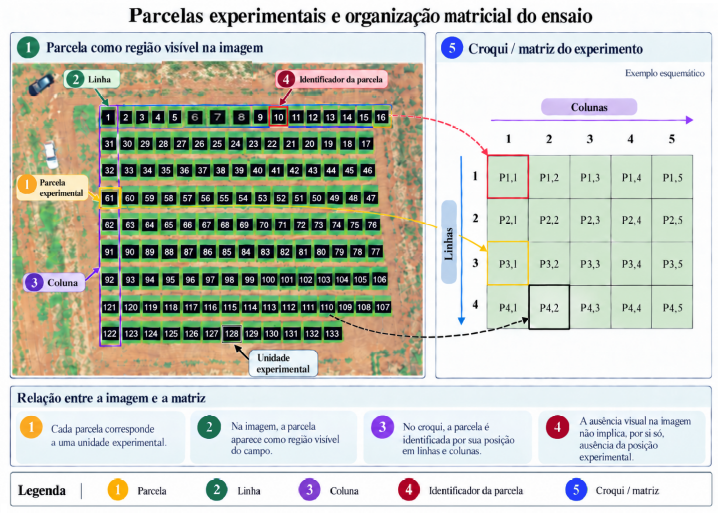
\includegraphics[width=0.9\textwidth]{figuras/figura03.png}
  \caption{Representa\c{c}\~ao da organiza\c{c}\~ao matricial de parcelas experimentais em ortomosaico obtido por drone.}
  \label{fig:organizacao-matricial}
  \fonte{Elaborado pelo autor (2026).}
\end{figure}

A fenotipagem vegetal compreende a obten\c{c}\~ao e an\'alise de caracter\'isticas observ\'aveis resultantes da intera\c{c}\~ao entre componentes gen\'eticos e condi\c{c}\~oes ambientais. Quando o n\'umero de materiais avaliados cresce, a quantidade de observa\c{c}\~oes necess\'arias cresce na mesma propor\c{c}\~ao, configurando um dos problemas reconhecidos para aproveitar plenamente os avan\c{c}os da gen\'etica e do melhoramento de plantas \citep{araus2014}. A fenotipagem de alto rendimento, ou \textit{high-throughput phenotyping}, designa o conjunto de estrat\'egias que responde a esse problema pela integra\c{c}\~ao de sensores, plataformas de aquisi\c{c}\~ao e m\'etodos computacionais, ampliando a escala e a velocidade com que as caracter\'isticas s\~ao registradas. Seu prop\'osito n\~ao \'e substituir as avalia\c{c}\~oes convencionais, mas aumentar a quantidade, a frequ\^encia ou a objetividade das observa\c{c}\~oes poss\'iveis em campo.

Para a an\'alise computacional de imagens, essa organiza\c{c}\~ao espacial \'e o que distingue duas representa\c{c}\~oes do mesmo experimento: a estrutura previamente definida no planejamento de campo e aquilo que pode ser efetivamente observado na imagem. Assim, a parcela deve ser compreendida simultaneamente como regi\~ao vis\'ivel e como posi\c{c}\~ao pertencente \`a organiza\c{c}\~ao espacial do ensaio, distin\c{c}\~ao que se tornar\'a central adiante, ao explicar por que uma aus\^encia visual n\~ao implica, necessariamente, que a posi\c{c}\~ao experimental correspondente deixou de existir.

\section{Sensoriamento remoto e aquisi\c{c}\~ao de imagens orbitais e de drone}
\label{sec:sensoriamento-remoto}

O sensoriamento remoto consiste na obten\c{c}\~ao de informa\c{c}\~oes sobre um alvo sem contato f\'isico direto com ele. Na an\'alise agr\'icola, sensores instalados em plataformas terrestres, a\'ereas ou orbitais permitem registrar propriedades da superf\'icie e da vegeta\c{c}\~ao a partir da radia\c{c}\~ao eletromagn\'etica refletida ou emitida.

Entre os sensores utilizados em aplica\c{c}\~oes agr\'icolas est\~ao as c\^ameras que operam na regi\~ao vis\'ivel do espectro e produzem imagens RGB. Essas imagens registram a intensidade da luz nas bandas correspondentes ao vermelho (RED), verde (GREEN) e azul (BLUE) e podem fornecer informa\c{c}\~oes relacionadas \`a estrutura aparente, cobertura e distribui\c{c}\~ao espacial da vegeta\c{c}\~ao.

Imagens de sat\'elite permitem observar extensas \'areas da superf\'icie em diferentes momentos, com caracter\'isticas de resolu\c{c}\~ao espacial, temporal e espectral que dependem do sensor e do produto disponibilizado. Para a identifica\c{c}\~ao de parcelas experimentais, a adequa\c{c}\~ao dessas imagens depende especialmente da rela\c{c}\~ao entre a resolu\c{c}\~ao espacial e o tamanho f\'isico das unidades que se pretende distinguir.

Em plataformas a\'ereas de baixa altitude, como drones, a combina\c{c}\~ao de m\'ultiplas fotografias pode produzir um ortomosaico, isto \'e, uma representa\c{c}\~ao cont\'inua da \'area constru\'ida a partir de m\'ultiplas imagens corrigidas e geometricamente combinadas. A utiliza\c{c}\~ao de ortomosaicos facilita a an\'alise de uma \'area experimental como uma \'unica superf\'icie visual, embora o processo de constru\c{c}\~ao possa introduzir distor\c{c}\~oes locais. \citet{mardanisamani2021}, por exemplo, observam que a forma\c{c}\~ao do ortomosaico a partir de v\'arias imagens pode produzir deforma\c{c}\~oes que dificultam o alinhamento preciso das micro parcelas com a estrutura te\'orica do campo.

Imagens orbitais oferecem uma rela\c{c}\~ao diferente entre cobertura, frequ\^encia e resolu\c{c}\~ao espacial em compara\c{c}\~ao a plataformas a\'ereas de baixa altitude; a adequa\c{c}\~ao de uma imagem para identificar parcelas individuais depende desta resolu\c{c}\~ao e do tamanho f\'isico das unidades experimentais, n\~ao apenas da origem do sensor. Foram utilizadas imagens orbitais, incluindo registros hist\'oricos disponibilizados pelo Google Earth, e ortomosaicos obtidos por drone em campos experimentais da Embrapa Gado de Corte.

\begin{figure}[htb]
  \centering
  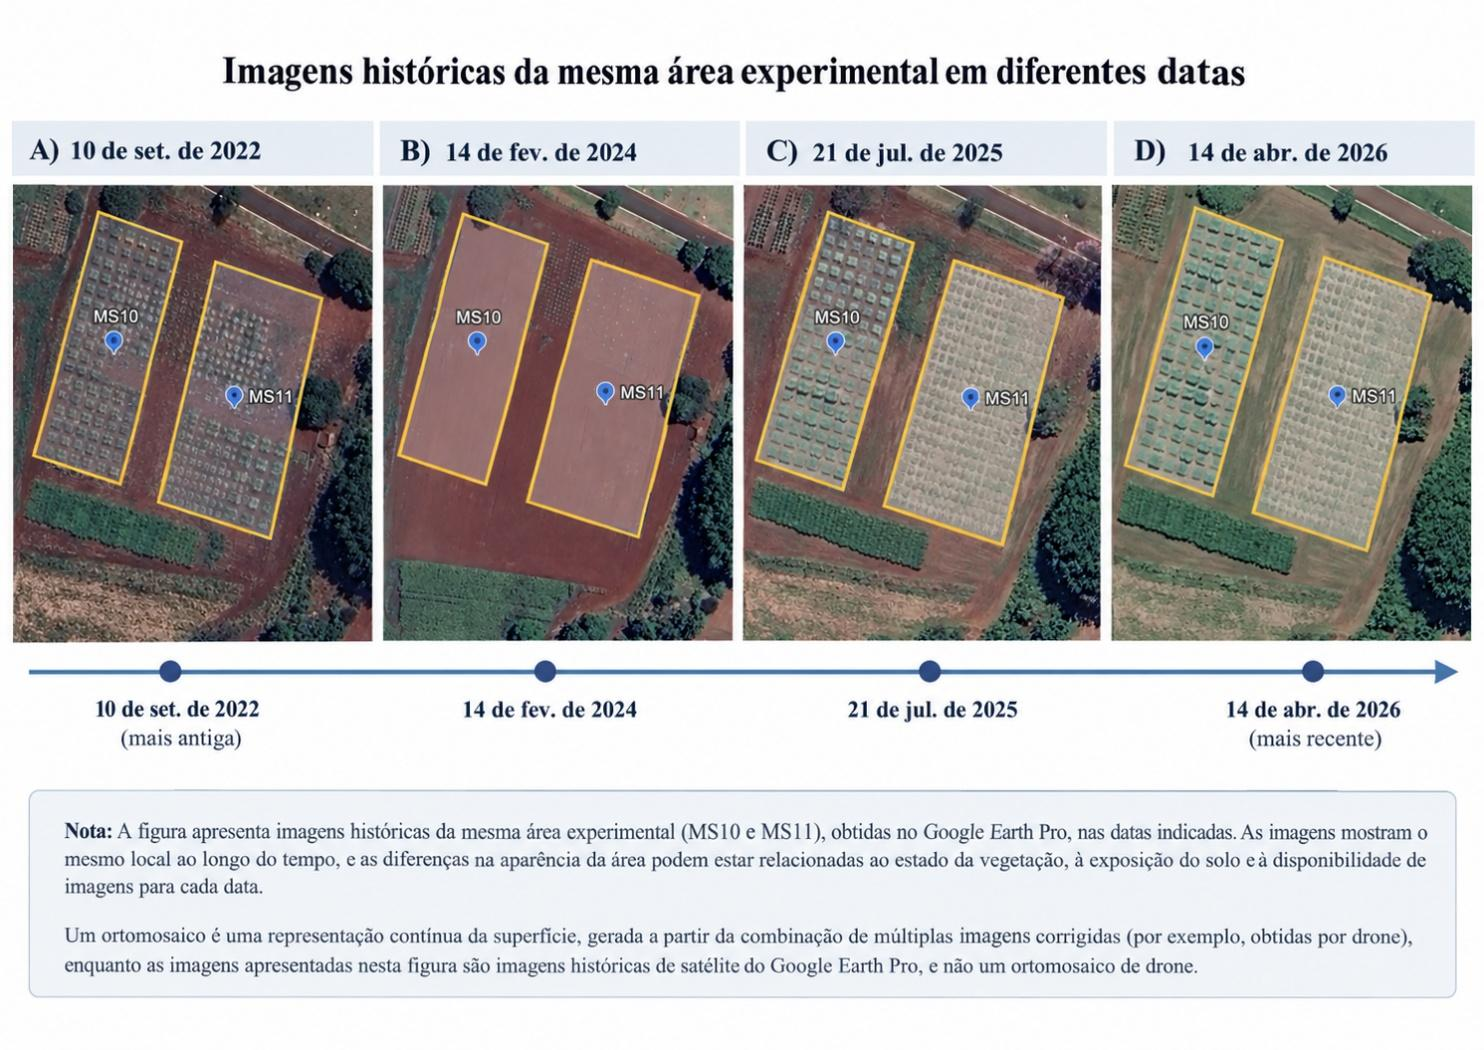
\includegraphics[width=0.95\textwidth]{figuras/figura04.jpg}
  \caption{Imagens hist\'oricas de sat\'elite da mesma \'area experimental em diferentes datas.}
  \label{fig:imagens-historicas}
  \fonte{Google Earth Pro, imagens hist\'oricas do ponto 20\textdegree 26'43.76"S, 54\textdegree 43'11.38"W. Elabora\c{c}\~ao do autor.}
\end{figure}

\section{Resolu\c{c}\~ao espacial e \textit{Ground Sample Distance}}
\label{sec:resolucao-espacial}

A resolu\c{c}\~ao espacial descreve o n\'ivel de detalhe representado por uma imagem, isto \'e, a menor extens\~ao do terreno que pode ser distinguida em seus elementos. Em dados obtidos por sensores digitais, uma maneira de expressar essa rela\c{c}\~ao \'e por meio da Dist\^ancia de Amostragem do Solo, ou \textit{\textbf{Ground Sample Distance} (GSD)}, que representa a dimens\~ao f\'isica do terreno correspondente \`a dist\^ancia entre pixels adjacentes na imagem.

Um pixel \'e o menor elemento que comp\~oe uma imagem digital, ao qual se associa um valor de intensidade ou de cor. Um GSD menor indica que cada pixel corresponde a uma extens\~ao menor da superf\'icie e, portanto, que detalhes espaciais menores podem ser representados na imagem. A capacidade efetiva de distinguir determinado objeto, contudo, tamb\'em depende de outras caracter\'isticas da aquisi\c{c}\~ao, do sensor, da qualidade da imagem e das propriedades visuais do pr\'oprio alvo.

\begin{figure}[htb]
  \centering
  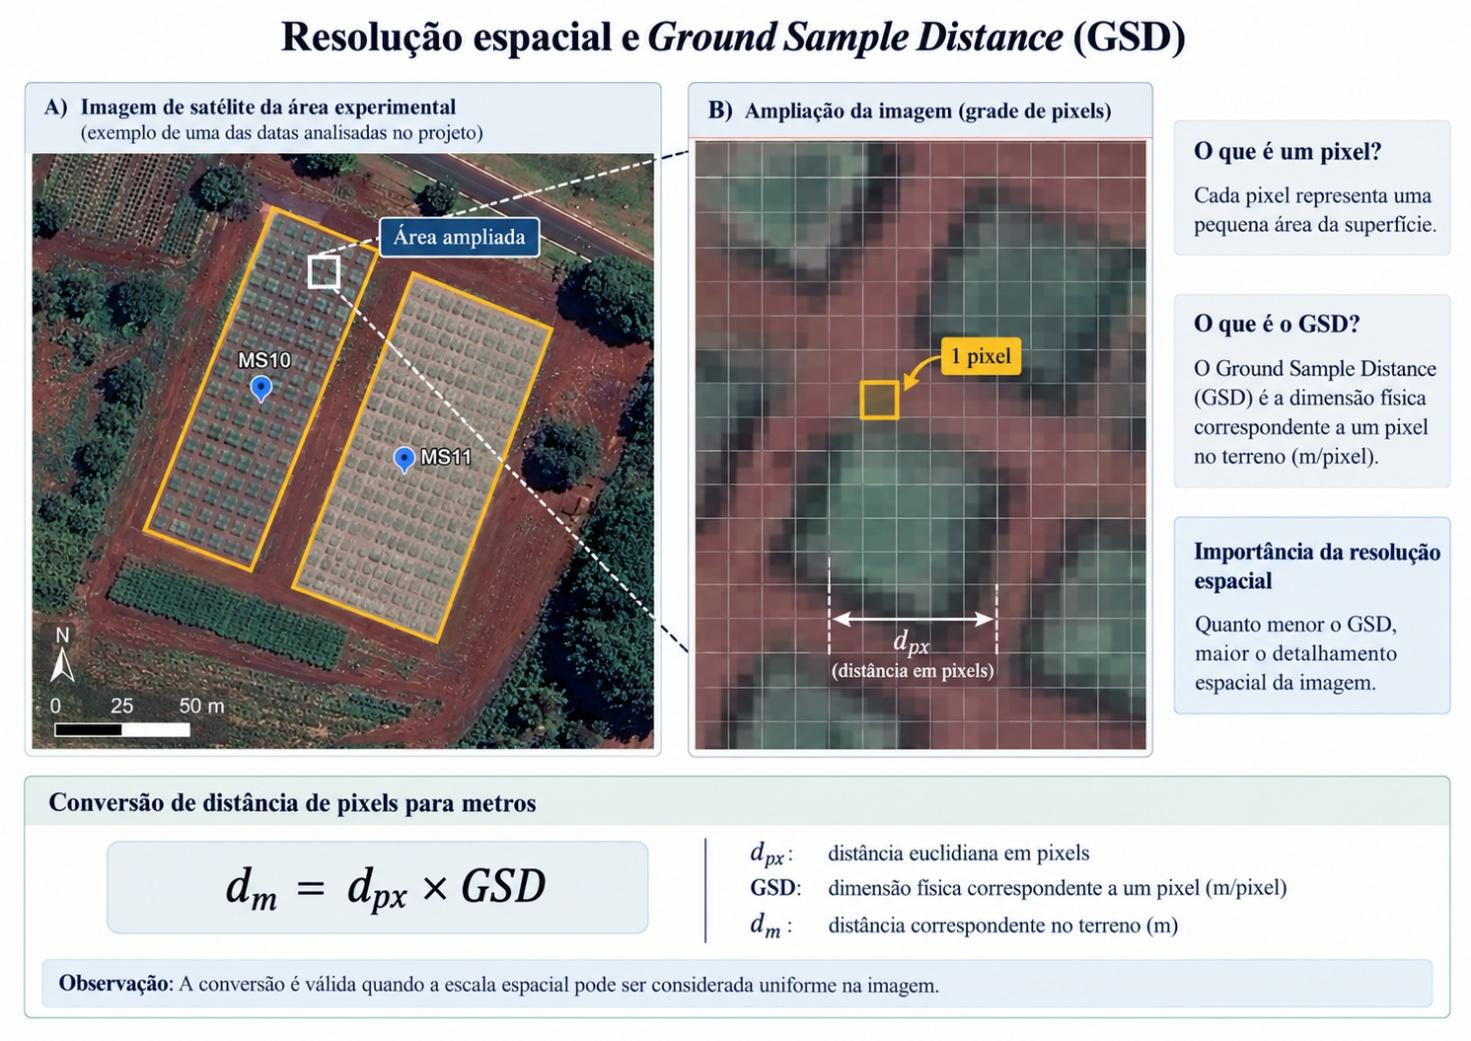
\includegraphics[width=0.9\textwidth]{figuras/figura05.jpg}
  \caption{Rela\c{c}\~ao entre resolu\c{c}\~ao espacial, pixel e Ground Sample Distance (GSD) em imagem de sat\'elite da \'area experimental.}
  \label{fig:gsd}
  \fonte{Elaborado pelo autor (2026).}
\end{figure}

O GSD pode ser utilizado para converter dist\^ancias em pixels para unidades f\'isicas quando a escala for conhecida e aplic\'avel \`a imagem medida. Sob a hip\'otese de uma escala espacial uniforme e igual nos dois eixos, se $d_{px}$ representa a dist\^ancia euclidiana em pixels e o GSD est\'a expresso em metros por pixel, obt\'em-se

\begin{equation}
  d_m = d_{px} \cdot \mathit{GSD}
  \label{eq:gsd}
\end{equation}

em que $d_m$ representa a dist\^ancia em metros.

Na implementa\c{c}\~ao do projeto, o GSD \'e tratado em metros por pixel e pode ser usado para converter dist\^ancias entre centros, em pixels, para metros.

No contexto deste trabalho, o GSD n\~ao \'e assumido como uma vari\'avel experimental cuja influ\^encia j\'a tenha sido sistematicamente avaliada. Sua import\^ancia est\'a principalmente na interpreta\c{c}\~ao espacial das medidas produzidas pelo sistema.

\section{Vis\~ao computacional, representa\c{c}\~ao de objetos e aprendizagem profunda (\textit{deep learning})}
\label{sec:visao-computacional}

A vis\~ao computacional formula diferentes tarefas a partir da mesma imagem, distinguindo-se pela natureza e pela precis\~ao da informa\c{c}\~ao produzida. Na classifica\c{c}\~ao, associa-se um r\'otulo ao conte\'udo global da imagem; na detec\c{c}\~ao, cada inst\^ancia \'e associada a uma classe e a uma regi\~ao espacial, geralmente uma caixa delimitadora; na segmenta\c{c}\~ao de inst\^ancias, acrescenta-se uma m\'ascara por objeto, isto \'e, um conjunto de pixels marcados como pertencentes \`aquele objeto espec\'ifico, o que distingue indiv\'iduos de uma mesma classe. O \textbf{Mask R-CNN}, arquitetura que estende um detector de duas etapas com um ramo dedicado \`a predi\c{c}\~ao dessas m\'ascaras, \'e um exemplo consolidado dessa formula\c{c}\~ao, realizando detec\c{c}\~ao e segmenta\c{c}\~ao simultaneamente \citep{he2017}. Em sentido mais amplo, a localiza\c{c}\~ao de um objeto pode ainda ser reduzida a um conjunto de pontos ou a uma posi\c{c}\~ao pontual, utilizada nesta pesquisa para sintetizar a localiza\c{c}\~ao de uma parcela.

Essa separa\c{c}\~ao \'e crucial, pois a caixa delimitadora, a m\'ascara de segmenta\c{c}\~ao e a representa\c{c}\~ao por ponto oferecem distintas granularidades de dados. Enquanto a caixa define a \'area espacial de forma resumida, a m\'ascara detalha a regi\~ao pixel a pixel, e o ponto apenas indica a posi\c{c}\~ao, sem capturar a forma ou o tamanho. N\~ao existe uma abordagem intrinsecamente melhor que as outras; a escolha ideal reside na aplica\c{c}\~ao espec\'ifica que se pretende executar.

Redes Neurais Convolucionais (\textbf{CNN}) aprendem representa\c{c}\~oes a partir dos dados. O treinamento utiliza uma fun\c{c}\~ao de perda, \textit{loss}, que quantifica a discrep\^ancia entre a sa\'ida produzida e a resposta esperada. A retropropaga\c{c}\~ao aplica a regra da cadeia para calcular os gradientes dessa perda em rela\c{c}\~ao aos par\^ametros da rede; o otimizador utiliza essas informa\c{c}\~oes para atualizar os par\^ametros \citep{pytorch2024}. Essa capacidade, por\'em, n\~ao garante robustez a condi\c{c}\~oes representadas no treinamento: a generaliza\c{c}\~ao precisa ser avaliada sobre dados suficientemente independentes daqueles usados no ajuste do modelo.

Uma caixa horizontal (\textit{\textbf{Horizontal Bounding Box}, HBB}) permanece alinhada aos eixos da imagem e pode ser descrita por

\begin{equation}
  b_{HBB} = \left(x_c, y_c, w, h\right)
  \label{eq:hbb}
\end{equation}

onde $x_c$ e $y_c$ s\~ao as coordenadas do centro e $w$ e $h$ s\~ao largura e altura.

Quando o objeto tem orienta\c{c}\~ao distinta da dos eixos, essa representa\c{c}\~ao pode incluir uma quantidade maior de regi\~ao externa ao objeto. A \textit{\textbf{Oriented Bounding Box} (OBB)} acrescenta a orienta\c{c}\~ao:

\begin{equation}
  b_{OBB} = \left(x_c, y_c, w, h, \theta\right)
  \label{eq:obb}
\end{equation}

reduzindo essa regi\~ao externa para objetos rotacionados, situa\c{c}\~ao particularmente estudada em imagens a\'ereas de alta densidade \citep{ding2019}. Essa propriedade geom\'etrica n\~ao implica que a OBB seja necessariamente superior \`a HBB ou \`a segmenta\c{c}\~ao de inst\^ancias.

\begin{figure}[htb]
  \centering
  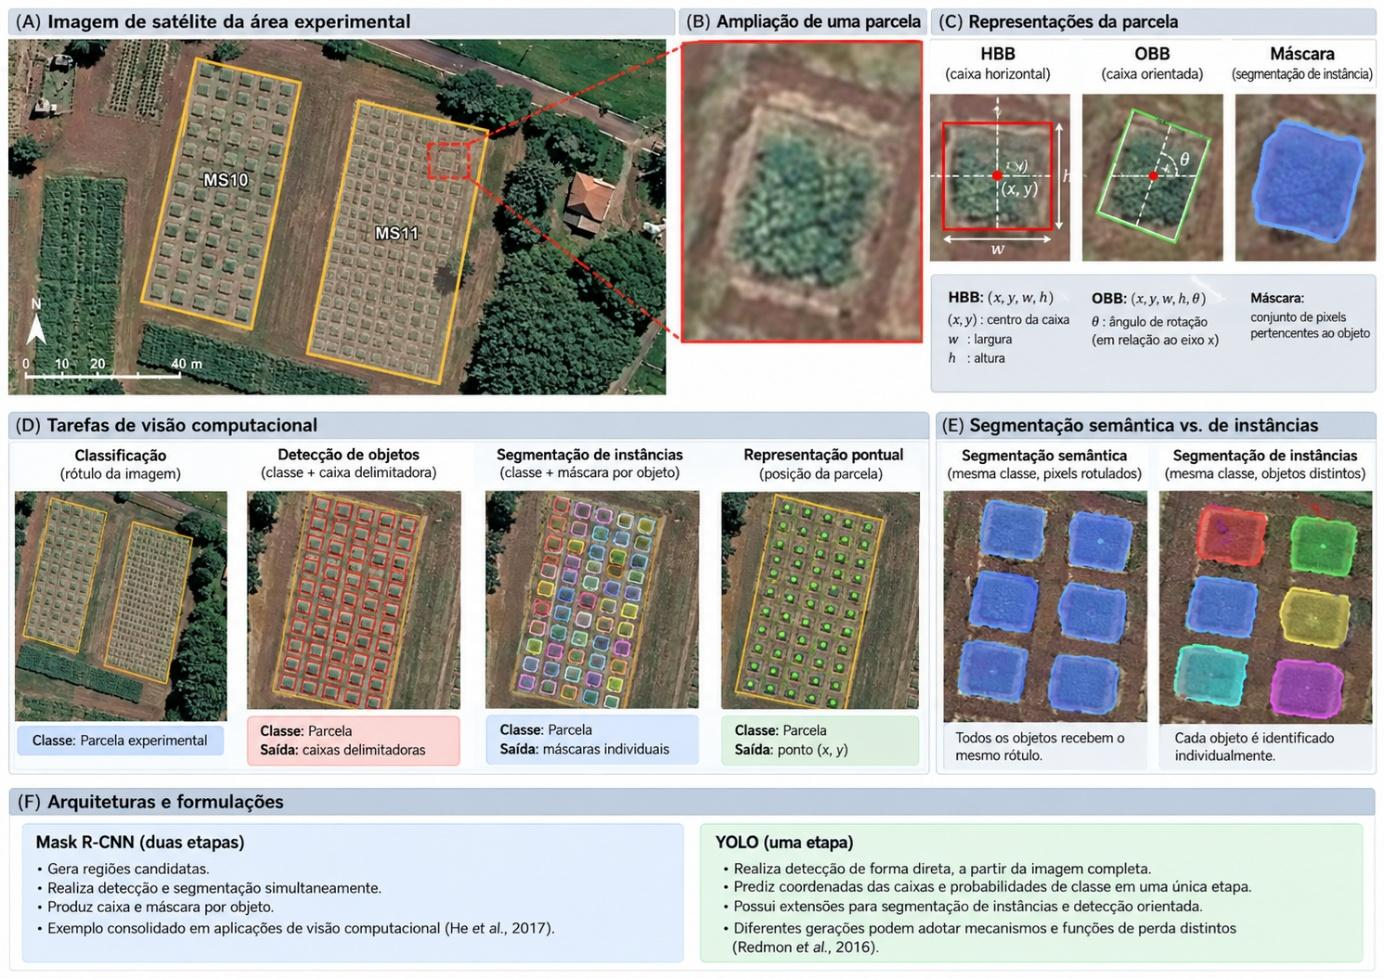
\includegraphics[width=0.95\textwidth]{figuras/figura06.jpg}
  \caption{Representa\c{c}\~oes de objetos em vis\~ao computacional aplicadas \`a identifica\c{c}\~ao de parcelas experimentais em imagens orbitais.}
  \label{fig:representacoes-objetos}
  \fonte{Elaborado pelo autor (2026).}
\end{figure}

Na segmenta\c{c}\~ao sem\^antica, pixels da mesma categoria recebem o mesmo r\'otulo independentemente de pertencerem a objetos fisicamente distintos; a segmenta\c{c}\~ao de inst\^ancias preserva, al\'em da categoria, a identidade individual de cada objeto. Essa distin\c{c}\~ao \'e relevante para experimentos agr\'icolas em que todas as parcelas compartilham uma mesma classe sem\^antica, mas ainda precisam ser contadas e manipuladas individualmente. No conjunto de 277 imagens, as parcelas foram anotadas como quadril\'ateros sob uma \'unica classe; outras organiza\c{c}\~oes dos dados usam anota\c{c}\~oes poligonais ou pontuais.

O \textbf{\textit{YOLO} (\textit{You Only Look Once})} \'e uma fam\'ilia de detectores de est\'agio \'unicos, proposta originalmente por \citet{redmon2016}. Sua formula\c{c}\~ao trata a detec\c{c}\~ao como um problema de regress\~ao direta, isto \'e, a rede prediz de uma s\'o vez, a partir da imagem completa, as coordenadas das caixas e as probabilidades de classe, sem uma etapa separada de gera\c{c}\~ao de regi\~oes candidatas seguida de classifica\c{c}\~ao, como faziam abordagens anteriores. Tal formula\c{c}\~ao deu origem a uma fam\'ilia posteriormente estendida a segmenta\c{c}\~ao de inst\^ancias e detec\c{c}\~ao orientada. N\~ao \'e adequado, contudo, assumir que todas as gera\c{c}\~oes compartilham a mesma arquitetura interna ou diferem apenas em profundidade ou n\'umero de par\^ametros: cada gera\c{c}\~ao pode alterar mecanismos de extra\c{c}\~ao e fus\~ao de caracter\'isticas, fun\c{c}\~oes de perda e estrat\'egias de atribui\c{c}\~ao. Por isso, os experimentos hist\'oricos do projeto com diferentes vers\~oes de YOLO n\~ao s\~ao assumidos de forma que possam ser diretamente compar\'aveis apenas por pertencerem \`a mesma fam\'ilia.

\section{Centros, centroides e representa\c{c}\~ao espacial}
\label{sec:centros-centroides}

Uma representa\c{c}\~ao bidimensional complexa pode ser sintetizada por meio de um ponto que indique sua posi\c{c}\~ao central. Conv\'em, por\'em, identificar sobre quais elementos esse ponto \'e calculado, pois procedimentos distintos recebem denomina\c{c}\~oes semelhantes.

Dado um conjunto de $K$ pontos de coordenadas $(x_i, y_i)$ que podem ser os v\'ertices de um pol\'igono ou os pixels de uma m\'ascara, a m\'edia aritm\'etica desses pontos \'e dada por:

\begin{equation}
  \bar{x} = \frac{1}{K}\sum_{i=1}^{K} x_i, \qquad \bar{y} = \frac{1}{K}\sum_{i=1}^{K} y_i
  \label{eq:centro-medio}
\end{equation}

Essa m\'edia representa o centro do conjunto de pontos considerados, de pesos iguais. Quando aplicada aos v\'ertices de um pol\'igono, ela fornece o centro desses v\'ertices, que n\~ao coincide, em geral, com o centr\'oide de \'area do pol\'igono, este \'ultimo obtido pela m\'edia ponderada de todos os seus pontos interiores. Quando a representa\c{c}\~ao utilizada \'e uma caixa delimitadora, seu centro pode ser obtido diretamente pelo ponto m\'edio entre seus limites.

Para uma mesma regi\~ao retangular uniforme, essas tr\^es posi\c{c}\~oes coincidem, em virtude da simetria da figura. Essa propriedade n\~ao se transfere automaticamente a um pol\'igono arbitr\'ario nem a uma m\'ascara de contorno irregular. A distin\c{c}\~ao importa quando posi\c{c}\~oes obtidas por caminhos diferentes s\~ao utilizadas em uma mesma etapa subsequente.

A redu\c{c}\~ao de uma parcela a um ponto facilita opera\c{c}\~oes de dist\^ancia, vizinhan\c{c}a e ordena\c{c}\~ao espacial. A dist\^ancia euclidiana entre dois pontos $p = (x_p, y_p)$ e $q = (x_q, y_q)$ \'e expressa por:

\begin{equation}
  d(p,q) = \sqrt{(x_p - x_q)^2 + (y_p - y_q)^2}
  \label{eq:distancia-centros}
\end{equation}

\begin{figure}[htb]
  \centering
  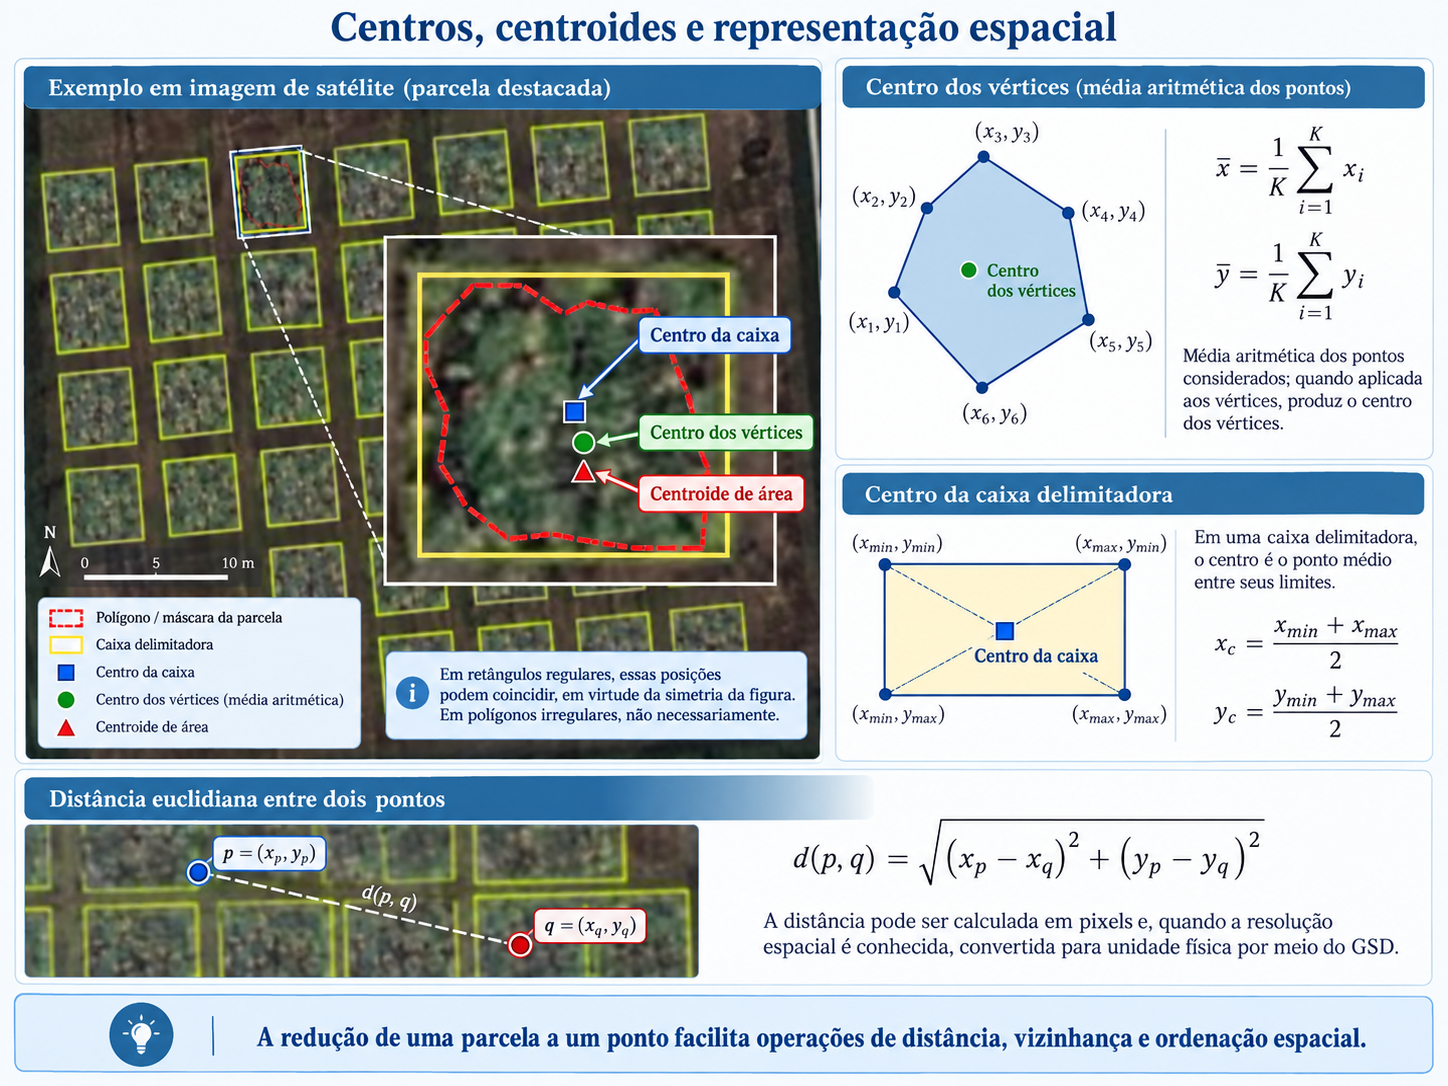
\includegraphics[width=0.9\textwidth]{figuras/figura07.png}
  \caption{Representa\c{c}\~ao de centros, centr\'oides e dist\^ancia euclidiana aplicados \`a localiza\c{c}\~ao espacial de parcelas experimentais em imagem orbital.}
  \label{fig:centros-centroides}
  \fonte{Elaborado pelo autor (2026).}
\end{figure}

Essa dist\^ancia pode ser calculada inicialmente em pixels e, quando a resolu\c{c}\~ao espacial \'e conhecida, convertida para unidade f\'isica por meio do GSD.

No sistema desenvolvido, medidas de dist\^ancia entre centros fazem parte das informa\c{c}\~oes utilizadas para avaliar a localiza\c{c}\~ao das detec\c{c}\~oes em rela\c{c}\~ao \`as anota\c{c}\~oes de refer\^encia.

\section{Organiza\c{c}\~ao espacial e estruturas em grade}
\label{sec:organizacao-espacial-grade}

A apar\^encia visual n\~ao \'e a \'unica fonte de informa\c{c}\~ao dispon\'ivel em um experimento agr\'icola. A disposi\c{c}\~ao planejada das parcelas tamb\'em estabelece rela\c{c}\~oes de posi\c{c}\~ao e vizinhan\c{c}a que podem ser utilizadas para interpretar as detec\c{c}\~oes produzidas a partir da imagem.

Em uma configura\c{c}\~ao organizada predominantemente por linhas e colunas, \'e poss\'ivel observar rela\c{c}\~oes entre posi\c{c}\~oes consecutivas, espa\c{c}amentos e alinhamentos. Essas regularidades podem fornecer informa\c{c}\~oes complementares quando se deseja estabelecer uma correspond\^encia entre objetos observados e posi\c{c}\~oes previstas.

\citet{mardanisamani2021} utiliza, por exemplo, a estrutura conhecida do experimento como ponto de partida para localizar as parcelas em ortomosaicos, refinando posteriormente a posi\c{c}\~ao da grade com base nas informa\c{c}\~oes da imagem. Este trabalho tenta demonstrar que a organiza\c{c}\~ao conhecida do campo, pode ser incorporada ao processo de localiza\c{c}\~ao, sem depender exclusivamente da an\'alise isolada de cada regi\~ao.

No problema investigado no escopo desta pesquisa, essa distin\c{c}\~ao se torna relevante quando uma parcela esperada n\~ao produz uma detec\c{c}\~ao. Se existem $N$ posi\c{c}\~oes previstas na organiza\c{c}\~ao experimental, mas apenas $N-K$ objetos s\~ao observados, o conjunto de detec\c{c}\~oes n\~ao representa integralmente a estrutura do experimento. Isso n\~ao significa que uma posi\c{c}\~ao ausente possa ser automaticamente reconstru\'ida apenas pela regularidade da grade. A infer\^encia de posi\c{c}\~oes faltantes constitui um problema adicional que precisa ser investigado e validado.

O interesse est\'a, portanto, em analisar de que maneira dist\^ancias, rela\c{c}\~oes de vizinhan\c{c}a, orienta\c{c}\~ao e conhecimento do croqui podem complementar a informa\c{c}\~ao visual. No projeto, essa dire\c{c}\~ao foi explorada por uma proposta referida como \textit{\textbf{Grid Completion}}, que consistia em estimar a dist\^ancia t\'ipica entre centros de parcelas vizinhas e, a partir dela, projetar as linhas e colunas da grade, de modo a ordenar as parcelas e estimar as posi\c{c}\~oes sem detec\c{c}\~ao correspondente.

\section{Informa\c{c}\~ao visual incompleta e posi\c{c}\~oes experimentais ausentes}
\label{sec:informacao-visual-incompleta}

A aus\^encia de evid\^encia visual e a inexist\^encia de uma posi\c{c}\~ao experimental representam situa\c{c}\~oes distintas. Uma parcela pode existir no planejamento do ensaio e, ainda assim, n\~ao produzir uma regi\~ao visual que um detector seja capaz de reconhecer. Nessa situa\c{c}\~ao, aquela posi\c{c}\~ao pode permanecer sem detec\c{c}\~ao correspondente, mesmo que a quantidade total de objetos preditos coincida com a de posi\c{c}\~oes previstas, pois detec\c{c}\~oes esp\'urias, isto \'e, predi\c{c}\~oes que n\~ao correspondem a nenhuma parcela, podem compensar numericamente as aus\^encias.

Essa diferen\c{c}a pode interferir principalmente em procedimentos de ordena\c{c}\~ao. Considere uma sequ\^encia de posi\c{c}\~oes $P_1, P_2, \ldots, P_N$. Se uma das posi\c{c}\~oes intermedi\'arias n\~ao possuir uma detec\c{c}\~ao associada e o algoritmo simplesmente ordenar os objetos observados de maneira consecutiva, as detec\c{c}\~oes posteriores poder\~ao ser associadas a identificadores incorretos. O problema passa, portanto, de uma tarefa exclusivamente visual para uma tarefa de correspond\^encia entre duas representa\c{c}\~oes: o conjunto de objetos observados e o conjunto de posi\c{c}\~oes previstas.

\begin{figure}[htb]
  \centering
  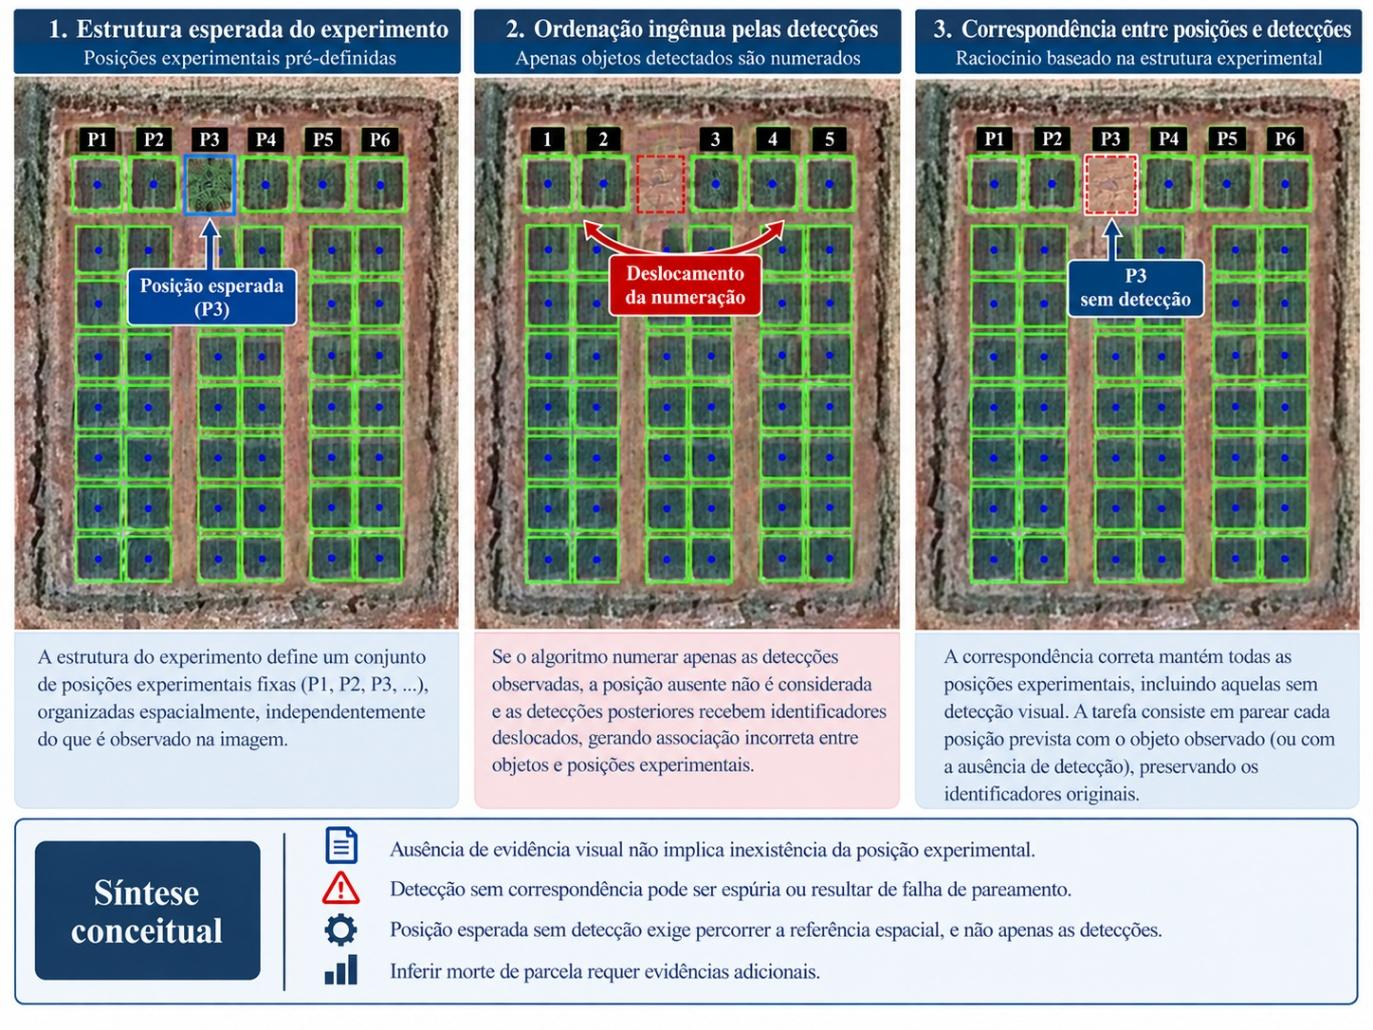
\includegraphics[width=0.95\textwidth]{figuras/figura08.jpg}
  \caption{Exemplo de deslocamento da numera\c{c}\~ao causado pela aus\^encia de detec\c{c}\~ao em uma posi\c{c}\~ao experimental.}
  \label{fig:deslocamento-numeracao}
  \fonte{Elaborado pelo autor (2026).}
\end{figure}

Conv\'em explicitar, neste ponto, que a afirma\c{c}\~ao de que uma parcela est\'a ausente ou morta, envolve uma cadeia de infer\^encias cujos elos dependem de evid\^encias pr\'oprias. Um objeto detectado que n\~ao encontra correspond\^encia em uma refer\^encia \'e o resultado de um procedimento de associa\c{c}\~ao, e pode decorrer de detec\c{c}\~ao esp\'uria, de cobertura parcial da refer\^encia ou de falha de pareamento. Um identificador da refer\^encia sem detec\c{c}\~ao associada \'e informa\c{c}\~ao de sentido oposto, e exige que o procedimento percorra a refer\^encia, e n\~ao apenas as detec\c{c}\~oes.

Uma posi\c{c}\~ao esperada sem evid\^encia visual \'e uma afirma\c{c}\~ao sobre o delineamento experimental, que pressup\~oe conhecimento da estrutura esperada. E a morte de uma parcela \'e uma afirma\c{c}\~ao agron\^omica, que pressup\~oe, al\'em da aus\^encia de evid\^encia visual, que essa aus\^encia n\~ao decorra de limita\c{c}\~ao do sensor, de oclus\~ao, de est\'agio fenol\'ogico ou de falha do detector. A passagem de um n\'ivel ao seguinte n\~ao \'e autom\'atica. Essa distin\c{c}\~ao orienta o projeto, contudo, o tratamento de posi\c{c}\~oes ausentes ainda n\~ao foi completamente sanado.

\section{Mapas de confian\c{c}a e representa\c{c}\~oes gaussianas}
\label{sec:mapas-confianca}

A detec\c{c}\~ao por caixas ou m\'ascaras n\~ao \'e a \'unica maneira de representar objetos em uma imagem. Em problemas de contagem e localiza\c{c}\~ao de objetos densamente distribu\'idos, tamb\'em podem ser empregados mapas cont\'inuos nos quais a posi\c{c}\~ao dos objetos \'e codificada espacialmente.

Uma maneira de construir essa representa\c{c}\~ao consiste em associar uma resposta gaussiana ao centro de cada objeto anotado. Um n\'ucleo gaussiano \'e uma fun\c{c}\~ao que atinge valor m\'aximo em um ponto central e decai suavemente \`a medida que a dist\^ancia a esse ponto aumenta, com a taxa desse decaimento controlada por um par\^ametro de dispers\~ao. Uma constru\c{c}\~ao poss\'ivel, a partir de $P$ posi\c{c}\~oes anotadas $(x_i, y_i)$, expressa-se como:

\begin{equation}
  F(x,y) = \sum_{i=1}^{P} \exp\left(-\frac{(x-x_i)^2 + (y-y_i)^2}{2\sigma^2}\right)
  \label{eq:mapa-confianca}
\end{equation}

em que $(x,y)$ \'e uma posi\c{c}\~ao qualquer do mapa, $(x_i, y_i)$ \'e a posi\c{c}\~ao do objeto $i$ e $\sigma$ controla a dispers\~ao espacial da resposta em torno dessa posi\c{c}\~ao.

\begin{figure}[htb]
  \centering
  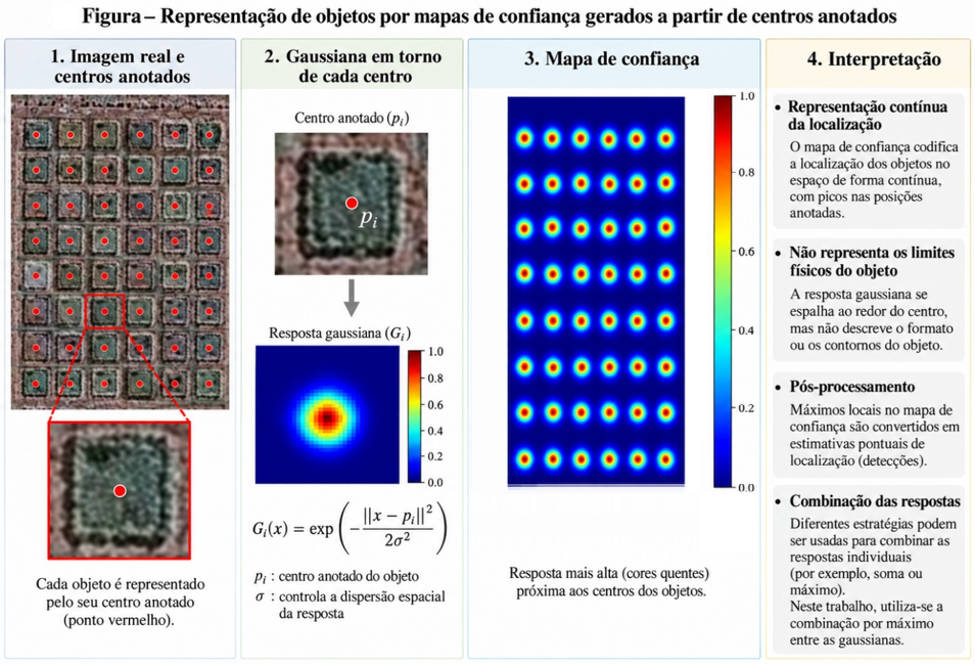
\includegraphics[width=0.9\textwidth]{figuras/figura09.png}
  \caption{Constru\c{c}\~ao de mapas de confian\c{c}a a partir de centros anotados em imagem real de parcelas experimentais.}
  \label{fig:mapas-confianca}
  \fonte{Elaborado pelo autor (2026).}
\end{figure}

Essa soma \'e uma entre outras formas poss\'iveis de combinar as respostas individuais. A implementa\c{c}\~ao do projeto n\~ao a utiliza diretamente, alternativamente, ela combina as respostas pelo valor m\'aximo em cada ponto. A escolha entre uma e outra altera o significado do mapa resultante, especialmente em regi\~oes densas, e a formula\c{c}\~ao supracitada n\~ao deve ser interpretada como descri\c{c}\~ao do procedimento local.

A representa\c{c}\~ao n\~ao delimita os limites f\'isicos do objeto. O mapa fornece uma indica\c{c}\~ao cont\'inua da intensidade da resposta associada \`a localiza\c{c}\~ao dos objetos; na implementa\c{c}\~ao, esses valores s\~ao amostrados em uma grade de pixels e utilizados para produzir estimativas pontuais por p\'os-processamento. Esses valores n\~ao constituem probabilidades calibradas pelo simples fato de serem designados como confian\c{c}a, e sua soma n\~ao corresponde necessariamente a uma contagem de objetos.

\citet{arruda2022} utilizaram essa ideia no contexto de contagem e localiza\c{c}\~ao de objetos em cen\'arios de elevada densidade, combinando enriquecimento dos mapas de caracter\'isticas com refinamento multiest\'agio de mapas de confian\c{c}a, avaliado em conjuntos de imagens de \'arvores e ve\'iculos. Essa abordagem \'e conceitualmente diferente da previs\~ao de uma caixa delimitadora, pois o objeto \'e representado principalmente por sua ocorr\^encia espacial, o que motivou sua considera\c{c}\~ao no desenvolvimento do projeto, dado o interesse em trabalhar com centros e com a localiza\c{c}\~ao de objetos distribu\'idos espacialmente.

\section{\textit{MultiStageRefinementNet}}
\label{sec:multistagerefinementnet}

\citet{arruda2022} prop\~oe uma abordagem para contagem e localiza\c{c}\~ao de objetos densamente distribu\'idos, baseada em redes neurais convolucionais e refinamento sucessivo de mapas de confian\c{c}a. Redes neurais convolucionais s\~ao arquiteturas que aplicam filtros aprendidos sobre regi\~oes locais da imagem, compondo representa\c{c}\~oes progressivamente mais abstratas a partir de padr\~oes visuais elementares.

A arquitetura proposta organiza-se em tr\^es componentes. Um extrator de caracter\'isticas reduz a resolu\c{c}\~ao espacial da imagem de entrada e produz uma representa\c{c}\~ao intermedi\'aria. Um m\'odulo de agrega\c{c}\~ao em pir\^amide, denominado \textit{\textbf{Pyramid Pooling Module}} \citep{zhao2017}, combina informa\c{c}\~oes obtidas por agrupamento em diferentes escalas, incorporando \`a representa\c{c}\~ao contexto de extens\~oes variadas. Uma sequ\^encia de est\'agios de refinamento, produz mapas de confian\c{c}a sucessivos, em que cada est\'agio recebe a sa\'ida do m\'odulo de agrega\c{c}\~ao e, a partir do segundo, o mapa produzido pelo est\'agio anterior.

Os alvos de treinamento de cada est\'agio s\~ao constru\'idos com valores decrescentes de $\sigma$, de modo que os est\'agios iniciais aprendam uma localiza\c{c}\~ao aproximada e os finais a refinem. Em vez de produzir uma \'unica estimativa espacial e encerr\'a-la, os est\'agios sucessivos procuram refinar as respostas geradas, favorecendo a localiza\c{c}\~ao de objetos em regi\~oes densas. A sa\'ida da rede \'e um mapa de confian\c{c}a representado em uma grade de pixels; as posi\c{c}\~oes dos objetos s\~ao obtidas em etapa posterior, pela identifica\c{c}\~ao de m\'aximos locais.

\'E importante diferenciar essa arquitetura, tal como descrita na publica\c{c}\~ao, da implementa\c{c}\~ao incorporada ao projeto. No m\'etodo publicado, o extrator de caracter\'isticas baseia-se na \textit{\textbf{VGG19}} \citep{simonyan2015}, arquitetura convolucional profunda de camadas sequenciais amplamente utilizada como extrator pr\'e-treinado. Na implementa\c{c}\~ao do projeto, a configura\c{c}\~ao padr\~ao utiliza um extrator simplificado, inspirado na VGG19 e sem pesos pr\'e-treinados, e houve tamb\'em treinamentos com essa arquitetura pr\'e-treinada.

A denomina\c{c}\~ao \textit{MultiStageRefinementNet} \'e a empregada no c\'odigo do projeto, e n\~ao necessariamente a utilizada na publica\c{c}\~ao de refer\^encia. A implementa\c{c}\~ao local foi desenvolvida em \textit{TensorFlow} e \textit{Keras} e permaneceu separada do fluxo principal, desenvolvido em \textit{PyTorch}.

No contexto desta pesquisa, essa abordagem constitui uma fam\'ilia metodol\'ogica diferente da detec\c{c}\~ao e da segmenta\c{c}\~ao baseadas em YOLO, pois privilegia a representa\c{c}\~ao espacial baseada em pontos e mapas de confian\c{c}a, sem delimitar a extens\~ao dos objetos.

\section{Classifica\c{c}\~ao de imagens e \textit{EfficientNet}}
\label{sec:classificacao-efficientnet}

A classifica\c{c}\~ao de imagens associa uma entrada visual a uma categoria global. Essa tarefa difere da detec\c{c}\~ao e da segmenta\c{c}\~ao porque n\~ao exige localizar os objetos respons\'aveis pela decis\~ao: a sa\'ida \'e um r\'otulo atribu\'ido \`a imagem como um todo.

A fam\'ilia \textit{EfficientNet} foi proposta por \citet{tan2019} a partir da investiga\c{c}\~ao do escalonamento de redes neurais convolucionais. Os autores observam que aumentar isoladamente a profundidade da rede, sua largura ou a resolu\c{c}\~ao da entrada nem sempre produz a melhor rela\c{c}\~ao entre desempenho e custo computacional, e prop\~oem um esquema de escalonamento composto, no qual essas tr\^es dimens\~oes s\~ao ampliadas conjuntamente segundo coeficientes relacionados por um fator \'unico.

A \textit{EfficientNet-B0} corresponde ao modelo de menor escala dessa fam\'ilia, obtido por busca de arquitetura, e serve de base a partir da qual as demais variantes s\~ao constru\'idas pela aplica\c{c}\~ao daquele esquema de escalonamento. Redes dessa fam\'ilia s\~ao frequentemente empregadas como extratores de caracter\'isticas pr\'e-treinados, com substitui\c{c}\~ao da camada final para adapta\c{c}\~ao a uma tarefa espec\'ifica.

Neste trabalho, uma \textit{EfficientNet-B0} foi empregada como componente auxiliar para classifica\c{c}\~ao bin\'aria da dificuldade operacional das imagens, a partir de r\'otulos derivados do comportamento de um detector. A classifica\c{c}\~ao n\~ao constitui o n\'ucleo do problema cient\'ifico da pesquisa e, por isso, a fundamenta\c{c}\~ao conceitual necess\'aria para esse componente \'e limitada.

\section{M\'etricas de avalia\c{c}\~ao}
\label{sec:metricas-avaliacao}

A avalia\c{c}\~ao de sistemas de detec\c{c}\~ao, segmenta\c{c}\~ao e localiza\c{c}\~ao exige medidas que representem diferentes aspectos do erro. Uma \'unica m\'etrica raramente caracteriza integralmente o desempenho de um modelo.

\textbf{\textit{Intersection over Union} (IoU):} Essa m\'etrica mede o grau de sobreposi\c{c}\~ao entre duas regi\~oes, comparando a \'area compartilhada com a \'area total ocupada por ambas. Corresponde ao \'indice de Jaccard aplicado \`as regi\~oes. Para uma regi\~ao predita $A$ e uma regi\~ao de refer\^encia $B$:

\begin{equation}
  \mathit{IoU}(A,B) = \frac{|A \cap B|}{|A \cup B|}
  \label{eq:iou}
\end{equation}

O resultado varia entre 0 e 1. Valores mais pr\'oximos de 1 indicam maior sobreposi\c{c}\~ao. A \textit{IoU} pode ser calculada tanto sobre caixas delimitadoras quanto sobre m\'ascaras, e sua interpreta\c{c}\~ao depende da representa\c{c}\~ao utilizada e do limiar definido para considerar uma correspond\^encia v\'alida.

Precis\~ao (\textit{Precision}): Expressa a propor\c{c}\~ao de detec\c{c}\~oes consideradas corretas entre todas as detec\c{c}\~oes produzidas pelo modelo:

\begin{equation}
  \mathit{Precision} = \frac{TP}{TP + FP}
  \label{eq:precision}
\end{equation}

em que $TP$ representa verdadeiros positivos e $FP$ representa falsos positivos.

Recall: Expressa a propor\c{c}\~ao dos objetos de refer\^encia que receberam uma detec\c{c}\~ao considerada correspondente:

\begin{equation}
  \mathit{Recall} = \frac{TP}{TP + FN}
  \label{eq:recall}
\end{equation}

em que $FN$ representa falsos negativos.

F1-score (F1): Combina precis\~ao e \textit{recall} por meio da m\'edia harm\^onica:

\begin{equation}
  F_1 = 2\,\frac{\mathit{Precision} \cdot \mathit{Recall}}{\mathit{Precision} + \mathit{Recall}}
  \label{eq:f1}
\end{equation}

\begin{figure}[htb]
  \centering
  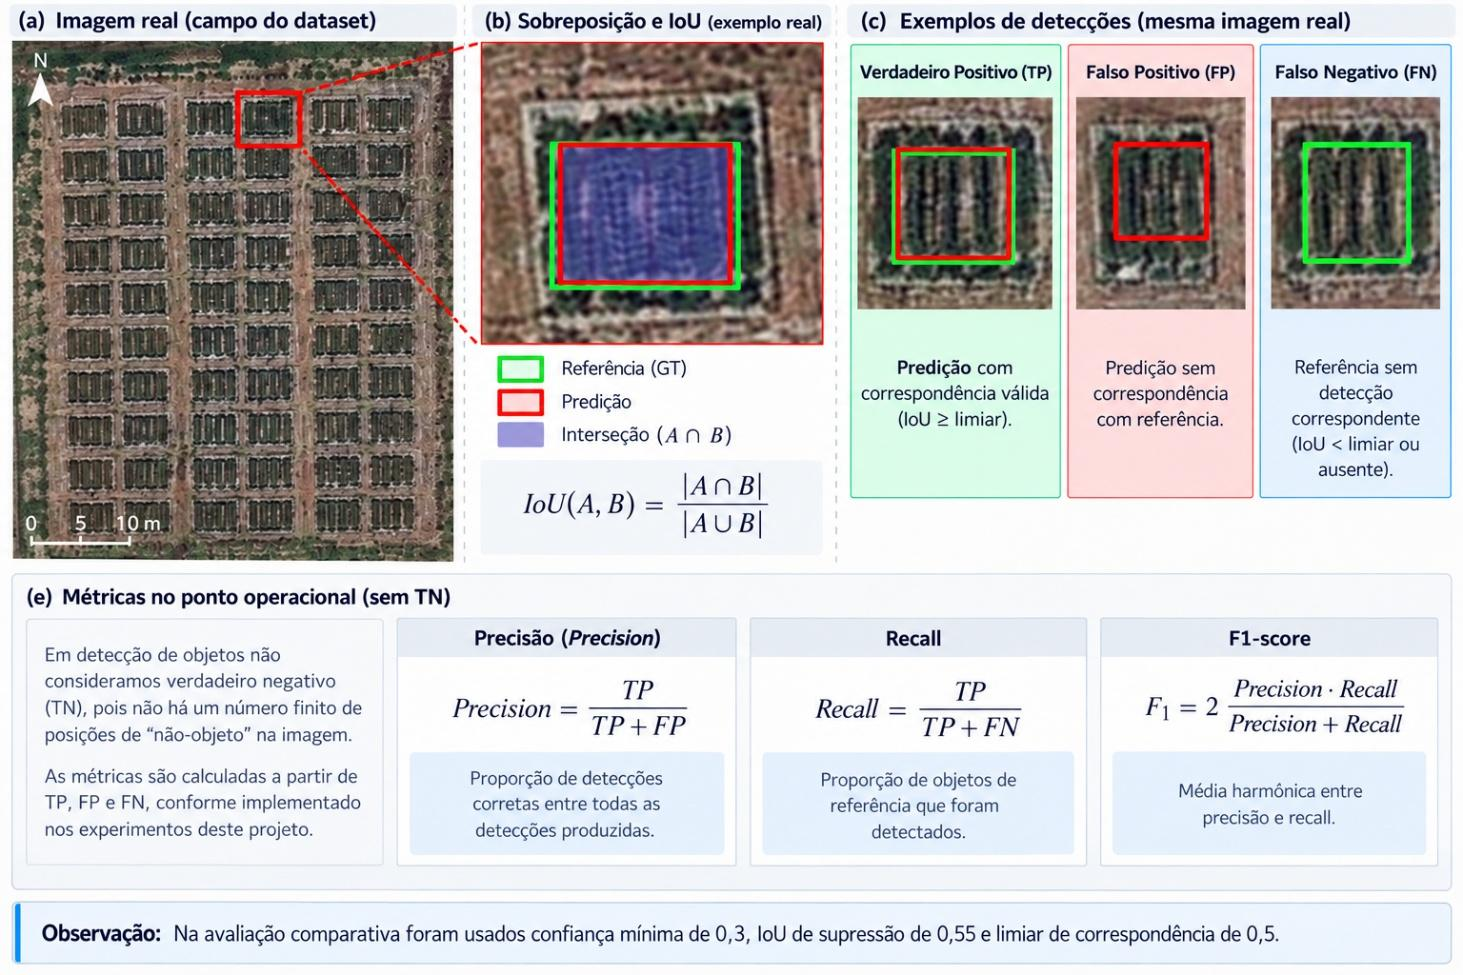
\includegraphics[width=0.95\textwidth]{figuras/figura10.jpg}
  \caption{Ilustra\c{c}\~ao conceitual de IoU, verdadeiro positivo, falso positivo, falso negativo, precis\~ao, recall e F1-score em detec\c{c}\~ao de parcelas experimentais.}
  \label{fig:iou-conceitual}
  \fonte{Elaborado pelo autor (2026).}
\end{figure}

Esse valor permite observar conjuntamente o efeito de falsos positivos e falsos negativos, embora n\~ao substitua a an\'alise individual de precis\~ao e \textit{recall}.

No que se refere em agrega\c{c}\~ao das medidas: Em conjuntos formados por v\'arias imagens, precis\~ao, \textit{recall} e \textit{F1} podem ser apresentados de maneiras distintas. As medidas globais s\~ao obtidas a partir das contagens acumuladas de verdadeiros positivos, falsos positivos e falsos negativos de todas as imagens consideradas. Alternativamente, podem ser calculadas m\'etricas individualmente para cada imagem e posteriormente obtida sua m\'edia, atribuindo o mesmo peso a cada imagem.

Essas formas de agrega\c{c}\~ao n\~ao s\~ao intercambi\'aveis: na agrega\c{c}\~ao global, os denominadores tamb\'em diferem entre as m\'etricas: a precis\~ao depende de $TP+FP$, enquanto o \textit{recall} depende de $TP+FN$. O F1 global \'e calculado a partir da precis\~ao e do \textit{recall} globais e, portanto, n\~ao corresponde necessariamente \`a m\'edia dos F1 obtidos individualmente por imagem.

Distin\c{c}\~ao semelhante ocorre para a \textit{IoU}: na avalia\c{c}\~ao utilizada neste projeto, s\~ao reportadas uma m\'edia da sobreposi\c{c}\~ao por imagem e uma m\'edia ponderada pelo n\'umero de correspond\^encias. A primeira atribui o mesmo peso \`as imagens consideradas, enquanto a segunda atribui maior peso \`as imagens com maior n\'umero de pares v\'alidos.

\textit{Average Precision e Mean Average Precision}: A \textit{Average Precision (AP)} resume a rela\c{c}\~ao entre precis\~ao e \textit{recall}, ao longo de diferentes n\'iveis de confian\c{c}a das predi\c{c}\~oes, condensando em um \'unico valor: a curva precis\~ao--recall. Protocolos como o \textit{PASCAL VOC} contribu\'iram para consolidar o uso dessa medida na avalia\c{c}\~ao de detectores \citep{everingham2010}.

Para um crit\'erio de sobreposi\c{c}\~ao fixado e $C$ classes, a m\'edia entre as AP das classes pode ser expressa por:

\begin{equation}
  mAP = \frac{1}{C}\sum_{c=1}^{C} AP_c
  \label{eq:map}
\end{equation}

Quando existe apenas uma classe, a m\'edia entre classes coincide numericamente com a \textit{AP} dessa classe para o mesmo crit\'erio de avalia\c{c}\~ao.

A avalia\c{c}\~ao pode ainda considerar diferentes limiares de \textit{IoU}: o \textbf{\textit{COCO}} \'e um conjunto p\'ublico de dados para reconhecimento de objetos que inclui tarefas de detec\c{c}\~ao e segmenta\c{c}\~ao \citep{lin2014}. Em seu protocolo oficial, uma das medidas sintetiza o desempenho em limiares de IoU entre 0,50 e 0,95, em incrementos de 0,05 \citep{cocoapi}. Esse crit\'erio \'e mais restritivo que uma avalia\c{c}\~ao realizada somente em \textit{IoU} igual a 0,50.

\'E necess\'ario distinguir duas varia\c{c}\~oes independentes: a primeira corresponde \`a confian\c{c}a das predi\c{c}\~oes, utilizada na constru\c{c}\~ao da curva precis\~ao--recall e, consequentemente, da \textit{AP}. A segunda corresponde ao crit\'erio de sobreposi\c{c}\~ao utilizado para determinar a qualidade espacial da detec\c{c}\~ao. Assim, \textbf{\textit{mAP@0,5}} e \textbf{\textit{mAP@0,5:0,95}} n\~ao representam apenas valores calculados em diferentes limiares de confian\c{c}a: diferem tamb\'em pelo conjunto de limiares de \textit{IoU} considerados.

Nos experimentos deste projeto s\~ao reportadas as duas medidas. Elas s\~ao obtidas por uma rotina de avalia\c{c}\~ao distinta da que calcula as m\'etricas por imagem em um ponto operacional; por isso, \textbf{\textit{mAP}}, precis\~ao global, \textit{recall, F1} e \textit{IoU} s\~ao interpretados de acordo com o protocolo que originou cada resultado.

Dist\^ancia entre centros: Quando o interesse inclui a qualidade da localiza\c{c}\~ao espacial, a dist\^ancia entre a posi\c{c}\~ao representativa de uma predi\c{c}\~ao e a posi\c{c}\~ao correspondente da refer\^encia fornece uma medida complementar \`a sobreposi\c{c}\~ao. Para dois pontos $p = (x_p, y_p)$ e $q = (x_q, y_q)$:

\begin{equation}
  d(p,q) = \sqrt{(x_p - x_q)^2 + (y_p - y_q)^2}
  \label{eq:distancia-centros-metrica}
\end{equation}

\begin{figure}[htb]
  \centering
  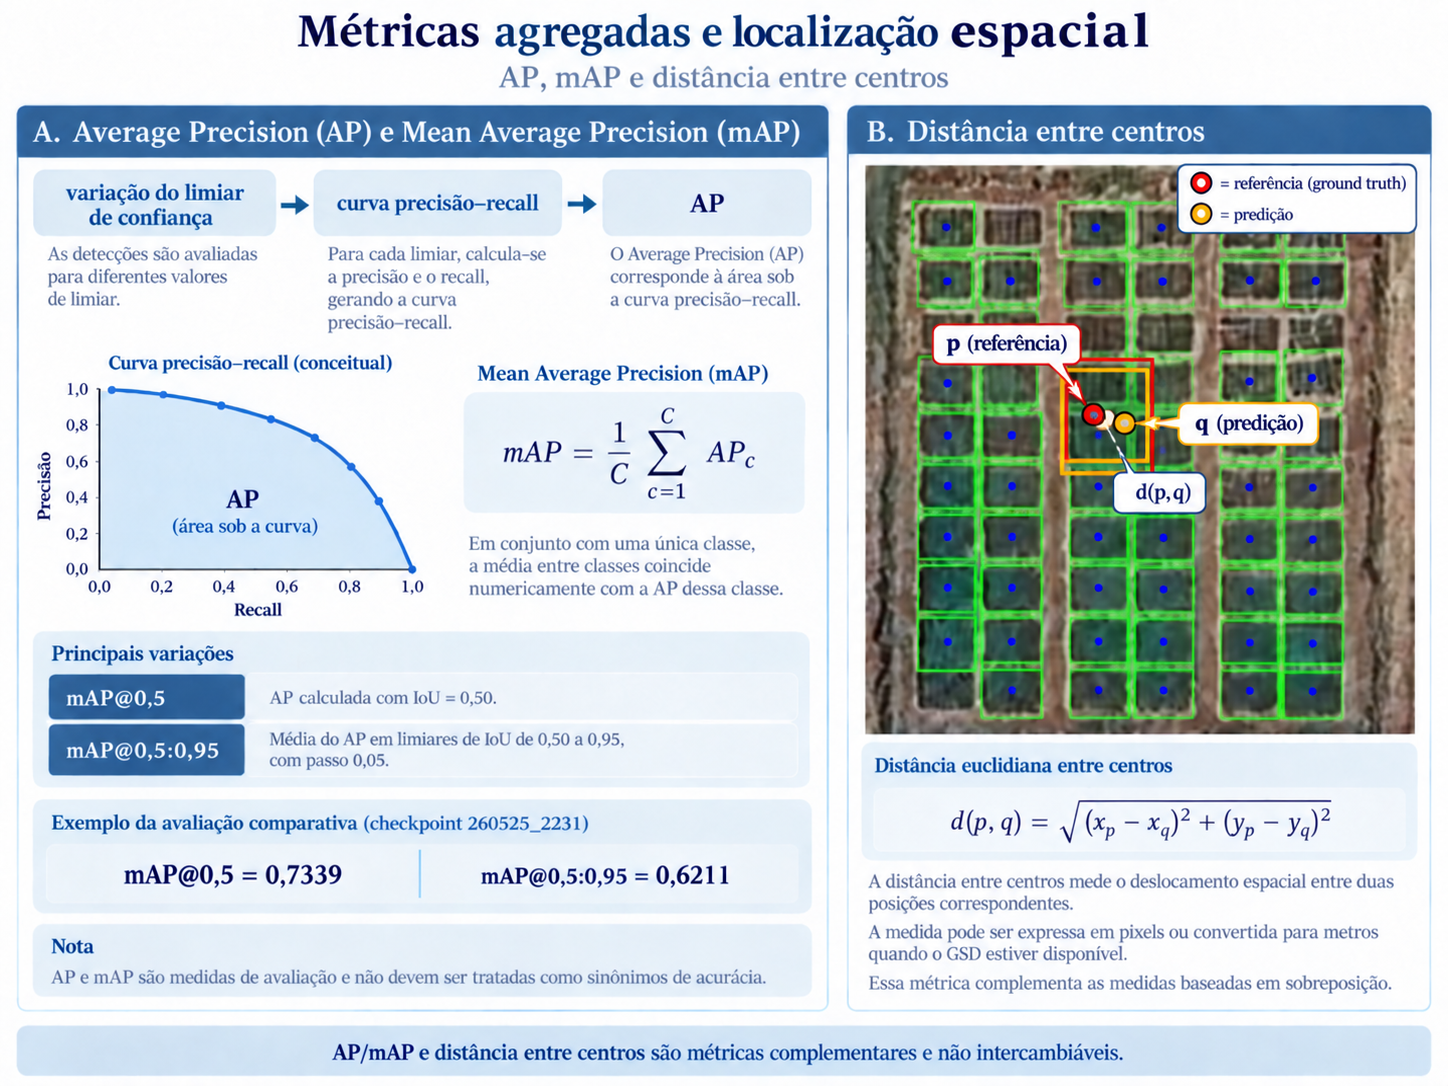
\includegraphics[width=0.9\textwidth]{figuras/figura11.png}
  \caption{Rela\c{c}\~ao entre AP, mAP e dist\^ancia entre centros na avalia\c{c}\~ao de detec\c{c}\~ao e localiza\c{c}\~ao espacial.}
  \label{fig:ap-map-distancia}
  \fonte{Elaborado pelo autor (2026).}
\end{figure}

A dist\^ancia \'e expressa em pixels, com a convers\~ao para unidades f\'isicas descrita na Se\c{c}\~ao~\ref{sec:resolucao-espacial}. Essa medida \'e relevante neste projeto porque uma parcela pode apresentar correspond\^encia visual satisfat\'oria e, ainda assim, possuir deslocamento espacial capaz de interferir nas etapas posteriores de associa\c{c}\~ao e organiza\c{c}\~ao das parcelas.

\section{Correspond\^encia entre previs\~oes e anota\c{c}\~oes}
\label{sec:correspondencia-previsoes}

Para calcular m\'etricas baseadas em verdadeiros positivos, falsos positivos e falsos negativos, \'e necess\'ario estabelecer quais predi\c{c}\~oes correspondem a quais anota\c{c}\~oes de refer\^encia.

Essa associa\c{c}\~ao pode ser realizada segundo diferentes crit\'erios. A \textit{Intersection over Union} (IoU) \'e empregada quando se deseja avaliar a sobreposi\c{c}\~ao entre regi\~oes, enquanto a dist\^ancia entre centros pode ser utilizada quando o interesse recai sobre a proximidade espacial das posi\c{c}\~oes representativas. No sistema desenvolvido existem procedimentos baseados nesses dois tipos de informa\c{c}\~ao. Na avalia\c{c}\~ao comparativa desta pesquisa, entretanto, as diferentes representa\c{c}\~oes de sa\'ida s\~ao convertidas para pol\'igonos e a associa\c{c}\~ao entre predi\c{c}\~oes e refer\^encias \'e determinada a partir da \textit{IoU}.

Quando cada predi\c{c}\~ao e cada anota\c{c}\~ao devem participar de no m\'aximo uma correspond\^encia, o problema assume uma estrutura de pareamento um-para-um. Os limiares utilizados para aceitar ou rejeitar uma associa\c{c}\~ao pertencem \`a configura\c{c}\~ao experimental e, portanto, n\~ao como valores te\'oricos universais.

Conv\'em distinguir dois problemas de correspond\^encia presentes neste trabalho. No primeiro, predi\c{c}\~oes s\~ao comparadas \`as anota\c{c}\~oes de refer\^encia da mesma imagem, com a finalidade de determinar acertos e erros de detec\c{c}\~ao. No segundo, objetos detectados em uma nova imagem de um campo s\~ao associados a uma refer\^encia espacial previamente numerada pelo operador, com o objetivo de transferir os identificadores das parcelas entre imagens. Essa refer\^encia \'e constru\'ida a partir das detec\c{c}\~oes numeradas e armazenada pelo sistema, n\~ao correspondendo a uma importa\c{c}\~ao autom\'atica do croqui agron\^omico.

Quando se busca minimizar conjuntamente o custo das correspond\^encias, a associa\c{c}\~ao pode ser formulada como um problema de atribui\c{c}\~ao linear, resolvido classicamente pelo m\'etodo h\'ungaro \citep{kuhn1955}. Nessa formula\c{c}\~ao, procura-se um conjunto de pares que minimize o custo total, impedindo que um mesmo elemento seja reutilizado em mais de uma correspond\^encia. Em matrizes retangulares, conjuntos de tamanhos diferentes permitem que elementos do conjunto maior perman\c{c}am sem par \citep{scipy}. A obten\c{c}\~ao da solu\c{c}\~ao de menor custo para a matriz constru\'ida n\~ao implica, entretanto, que os pares encontrados correspondam necessariamente \`as identidades corretas no delineamento experimental.

O segundo problema apresenta ainda uma dificuldade geom\'etrica: os conjuntos de pontos obtidos em imagens distintas de um mesmo campo podem apresentar diferen\c{c}as de posi\c{c}\~ao, escala e orienta\c{c}\~ao. O registro de conjuntos de pontos busca reduzir essas diferen\c{c}as antes da associa\c{c}\~ao. O m\'etodo \textit{Coherent Point Drift} (\textit{CPD}) \citep{myronenko2010} formula esse registro probabilisticamente, tratando os pontos de um conjunto como centr\'oides de uma mistura de distribui\c{c}\~oes gaussianas ajustada ao outro conjunto.

No procedimento implementado, o registro por \textit{CPD} \'e aplicado aos centros das detec\c{c}\~oes para aproximar o conjunto correspondente \`a nova imagem da refer\^encia espacial. A determina\c{c}\~ao das identidades ocorre posteriormente, por meio de uma fun\c{c}\~ao de custo e de uma atribui\c{c}\~ao um-para-um. Dessa forma, registro geom\'etrico e atribui\c{c}\~ao de identidade constituem etapas distintas: o primeiro aproxima espacialmente os conjuntos; o segundo determina quais elementos ser\~ao considerados correspondentes.

\section{Generaliza\c{c}\~ao e depend\^encia entre amostras}
\label{sec:generalizacao-dependencia}

O treinamento de um modelo de aprendizado supervisionado procura ajustar seus par\^ametros a partir de exemplos dispon\'iveis, mas o interesse cient\'ifico normalmente est\'a em seu comportamento sobre observa\c{c}\~oes que n\~ao participaram desse processo.

Por essa raz\~ao, os dados costumam ser separados em conjuntos com fun\c{c}\~oes distintas. O conjunto de treinamento \'e utilizado para atualizar os par\^ametros do modelo. O conjunto de valida\c{c}\~ao pode ser utilizado durante o desenvolvimento para sele\c{c}\~ao de configura\c{c}\~oes e acompanhamento do comportamento do treinamento. O conjunto de teste deve fornecer uma avalia\c{c}\~ao sobre dados preservados da etapa de ajuste.

\begin{figure}[htb]
  \centering
  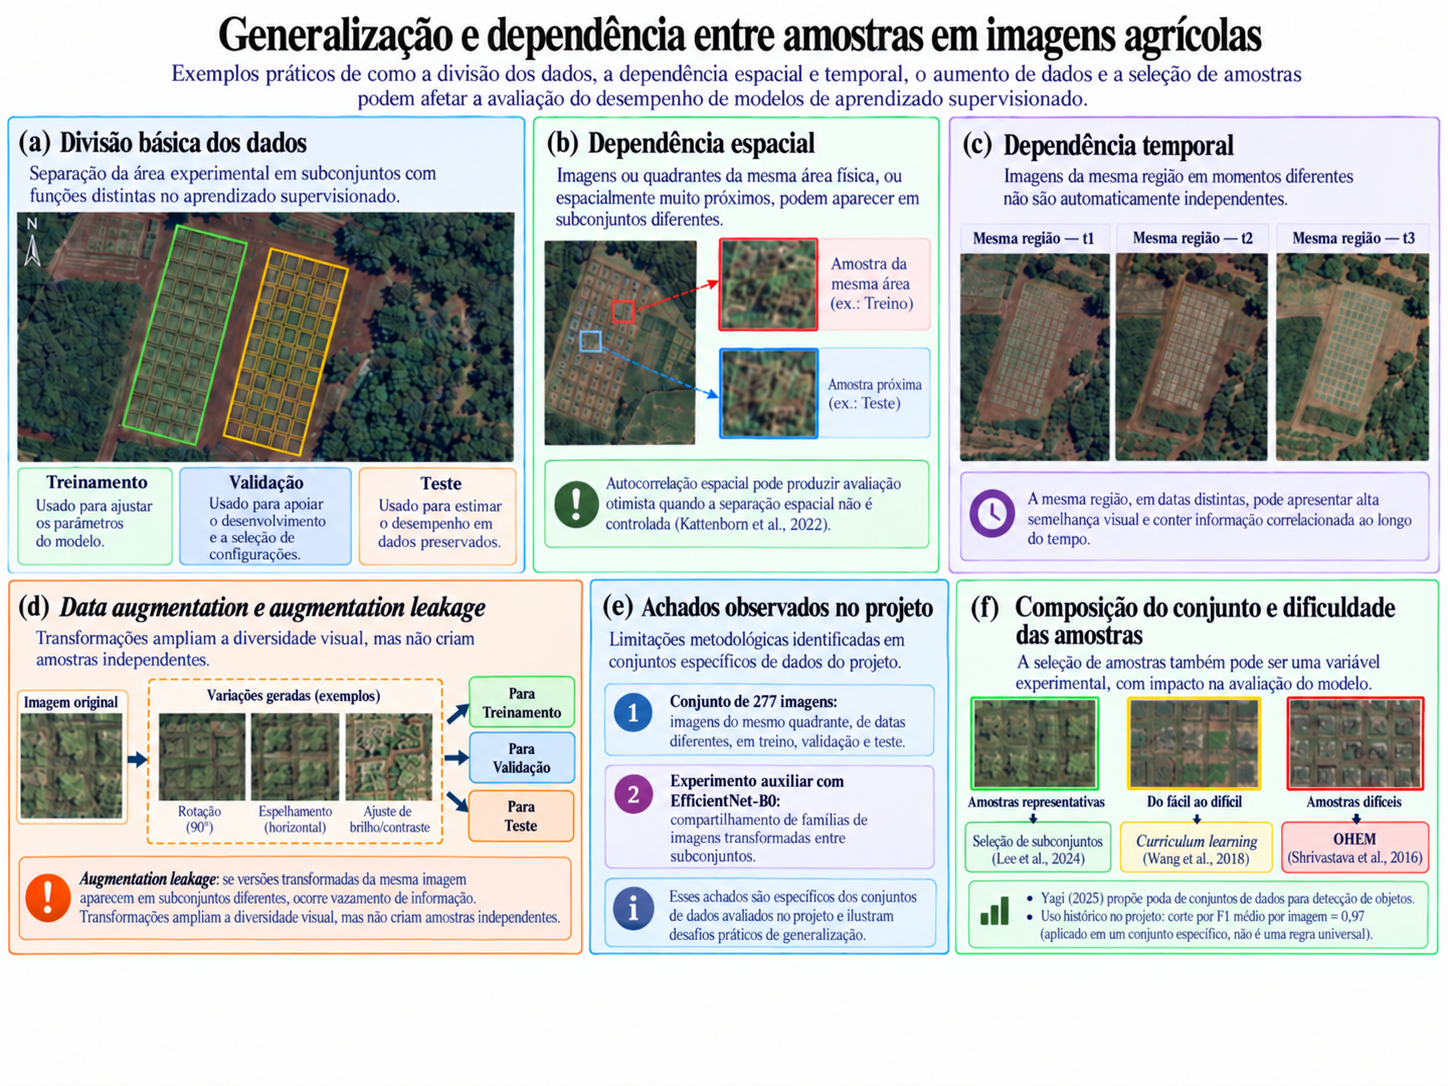
\includegraphics[width=0.95\textwidth]{figuras/figura12.png}
  \caption{Generaliza\c{c}\~ao, depend\^encia espacial e temporal, augmentation leakage e sele\c{c}\~ao de amostras no treinamento de modelos.}
  \label{fig:generalizacao-dependencia}
  \fonte{Elaborado pelo autor (2026).}
\end{figure}

A validade dessa avalia\c{c}\~ao depende n\~ao apenas de os arquivos terem nomes diferentes, mas tamb\'em do grau de independ\^encia entre as observa\c{c}\~oes. Em dados geoespaciais, imagens espacialmente pr\'oximas ou provenientes da mesma \'area podem compartilhar caracter\'isticas que tornam a tarefa de previs\~ao mais semelhante \`aquela observada no treinamento.

\citet{kattenborn2022} demonstram, em um problema de segmenta\c{c}\~ao com imagens de sensoriamento remoto, que a presen\c{c}a de amostras espacialmente autocorrelacionadas entre treinamento e valida\c{c}\~ao pode produzir avalia\c{c}\~oes mais otimistas do que aquelas obtidas quando a separa\c{c}\~ao espacial \'e considerada explicitamente.

Assim, quando imagens da mesma regi\~ao f\'isica aparecem em subconjuntos diferentes, n\~ao \'e poss\'ivel assumir automaticamente que o desempenho observado representa a capacidade de transfer\^encia para regi\~oes independentes. Isso tamb\'em n\~ao significa que o modelo necessariamente tenha memorizado a \'area. A conclus\~ao metodologicamente adequada \'e que a correla\c{c}\~ao entre as observa\c{c}\~oes reduz a independ\^encia da avalia\c{c}\~ao e limita a interpreta\c{c}\~ao das m\'etricas como estimativas de generaliza\c{c}\~ao espacial.

A depend\^encia entre observa\c{c}\~oes tamb\'em pode ocorrer no dom\'inio temporal. Imagens adquiridas na mesma regi\~ao em momentos distintos podem compartilhar padr\~oes de solo, organiza\c{c}\~ao das parcelas, limites f\'isicos e outras caracter\'isticas visuais. Quando essas observa\c{c}\~oes s\~ao distribu\'idas entre treinamento e teste, a interpreta\c{c}\~ao do desempenho deve considerar essa correla\c{c}\~ao.

O aumento de dados, \textit{data augmentation}, possui finalidade diferente. Trata-se da aplica\c{c}\~ao de transforma\c{c}\~oes \`as imagens dispon\'iveis, como rota\c{c}\~oes, espelhamentos, altera\c{c}\~oes de brilho ou outras perturba\c{c}\~oes, com o objetivo de ampliar a diversidade visual apresentada durante o treinamento sem exigir novas coletas.

Essas transforma\c{c}\~oes, entretanto, n\~ao produzem observa\c{c}\~oes independentes de sua imagem de origem. Imagens derivadas do mesmo original continuam compartilhando grande parte de seu conte\'udo. Quando derivados de uma mesma imagem s\~ao distribu\'idos entre treinamento e teste, ocorre uma forma de \textit{augmentation leakage}, pois o conjunto de teste passa a conter informa\c{c}\~ao fortemente relacionada a dados que tamb\'em participaram do treinamento.

A composi\c{c}\~ao do conjunto de treinamento tamb\'em pode ser tratada como vari\'avel experimental. Em detec\c{c}\~ao supervisionada, diferentes trabalhos utilizam dificuldade ou informatividade das amostras de formas distintas. O \textit{Online Hard Example Mining} prioriza exemplos dif\'iceis durante o treinamento de detectores \citep{shrivastava2016}. \citet{wang2018} organizam amostras segundo sua dificuldade em uma estrat\'egia de \textit{curriculum learning}. Em outra dire\c{c}\~ao, \citet{lee2024} investigam a sele\c{c}\~ao de subconjuntos representativos e diversos especificamente para detec\c{c}\~ao de objetos.

\citet{yagi2025}, em trabalho dispon\'ivel como \textit{preprint}, estende a discuss\~ao de \textit{dataset pruning} \`a detec\c{c}\~ao de objetos e prop\~oe o \textit{Variance-based Prediction Score}, calculado pela varia\c{c}\~ao, ao longo das \'epocas de treinamento, do \textit{IoU} ou da confian\c{c}a da predi\c{c}\~ao associada a cada objeto, com posterior agrega\c{c}\~ao das medidas dos objetos para o n\'ivel da imagem. Nesse \textit{score}, valores baixos correspondem a objetos detectados ou n\~ao detectados de forma consistente, e valores altos, a objetos de dificuldade intermedi\'aria; as imagens de menor escore s\~ao removidas. No \textit{PASCAL VOC}, a sele\c{c}\~ao por esse escore superou subconjuntos aleat\'orios de mesmo tamanho em todas as taxas de remo\c{c}\~ao avaliadas, mas permaneceu abaixo do conjunto completo. Em outro regime de aprendizagem, \citet{zhang2026} analisa, na aprendizagem contrastiva n\~ao supervisionada, pares de amostras de classes diferentes com alta similaridade e mostraram que a remo\c{c}\~ao ou o tratamento espec\'ifico desses pares pode melhorar a generaliza\c{c}\~ao. Esses trabalhos empregam tarefas, unidades de an\'alise e defini\c{c}\~oes de dificuldade distintas e n\~ao demonstram que exemplos dif\'iceis devam necessariamente ser exclu\'idos ou priorizados. Em conjunto, mostram que a contribui\c{c}\~ao das amostras depende do crit\'erio de sele\c{c}\~ao e que a composi\c{c}\~ao do conjunto de treinamento pode ser investigada como parte do pr\'oprio problema de aprendizagem.

Quando a dificuldade de uma imagem \'e estimada a partir do desempenho de um modelo, deve-se ainda considerar a independ\^encia entre o modelo utilizado para produzir essa estimativa e a imagem avaliada. Se uma imagem tiver participado do ajuste do detector que posteriormente \'e utilizado para classific\'a-la como f\'acil ou dif\'icil, a medida poder\'a refletir parcialmente o contato pr\'evio do modelo com aquela observa\c{c}\~ao. Por essa raz\~ao, nesta pesquisa o crit\'erio de sele\c{c}\~ao ser\'a calculado em imagens que n\~ao participaram do treinamento do modelo que as avalia, e o efeito da sele\c{c}\~ao ser\'a medido em grupos de teste separados.

As compara\c{c}\~oes das propostas futuras, permitir\~ao investigar se altera\c{c}\~oes na composi\c{c}\~ao do conjunto de treinamento afetam a capacidade de generaliza\c{c}\~ao do detector. A proposta n\~ao pressup\~oe que remover imagens consideradas dif\'iceis produzir\'a melhora: o efeito poder\'a ser positivo, negativo ou inexistente, e dever\'a ser determinado experimentalmente.

\chapter{Metodologia}
\label{cap:metodologia}

\section{Caracteriza\c{c}\~ao}
\label{sec:caracterizacao}

Foram investigados m\'etodos de vis\~ao computacional para identificar, delimitar, localizar e organizar espacialmente parcelas experimentais de forrageiras em imagens orbitais e de drone. Na continuidade proposta nesta qualifica\c{c}\~ao, a composi\c{c}\~ao do conjunto de treinamento passa a ser tratada como vari\'avel experimental, para avaliar se uma sele\c{c}\~ao de imagens orientada por um crit\'erio quantitativo de instabilidade das predi\c{c}\~oes altera a capacidade de generaliza\c{c}\~ao do detector. A identifica\c{c}\~ao das parcelas \'e tratada como etapa de suporte \`a an\'alise dos experimentos e \`a fenotipagem. O sistema n\~ao mede caracter\'isticas como biomassa, altura ou produtividade; seu objetivo \'e localizar e delimitar as parcelas nas imagens e associ\'a-las \`as unidades experimentais previstas no ensaio.

O desenvolvimento foi incremental. Em momentos distintos, foram investigadas a segmenta\c{c}\~ao de inst\^ancias, a detec\c{c}\~ao por caixas delimitadoras horizontais e orientadas, a detec\c{c}\~ao em cascata, a localiza\c{c}\~ao por mapas de confian\c{c}a e um classificador auxiliar de dificuldade das imagens. Tamb\'em foi implementado um procedimento que transfere identificadores de parcelas entre imagens de um mesmo campo a partir de uma refer\^encia numerada. Esses componentes n\~ao formam um fluxo \'unico: alguns foram implementados e avaliados, outros foram conduzidos como linhas independentes, e parte das propostas n\~ao chegou a ser implementada ainda.

\section{Vis\~ao geral}
\label{sec:visao-geral-metodologia}

O processo metodol\'ogico parte da imagem da \'area experimental e chega \`as informa\c{c}\~oes espaciais das parcelas (Figura~\ref{fig:processo-metodologico}). Compreende a obten\c{c}\~ao e a organiza\c{c}\~ao das imagens, a anota\c{c}\~ao das parcelas, a organiza\c{c}\~ao dos conjuntos de dados, o treinamento dos modelos, a extra\c{c}\~ao das posi\c{c}\~oes das parcelas a partir das sa\'idas, a avalia\c{c}\~ao das predi\c{c}\~oes em rela\c{c}\~ao \`as anota\c{c}\~oes de refer\^encia e a associa\c{c}\~ao das detec\c{c}\~oes \`a organiza\c{c}\~ao espacial do experimento. A avalia\c{c}\~ao de estrat\'egias de composi\c{c}\~ao do conjunto de treinamento \'e a etapa prevista para a continuidade do trabalho.

\begin{figure}[htb]
  \centering
  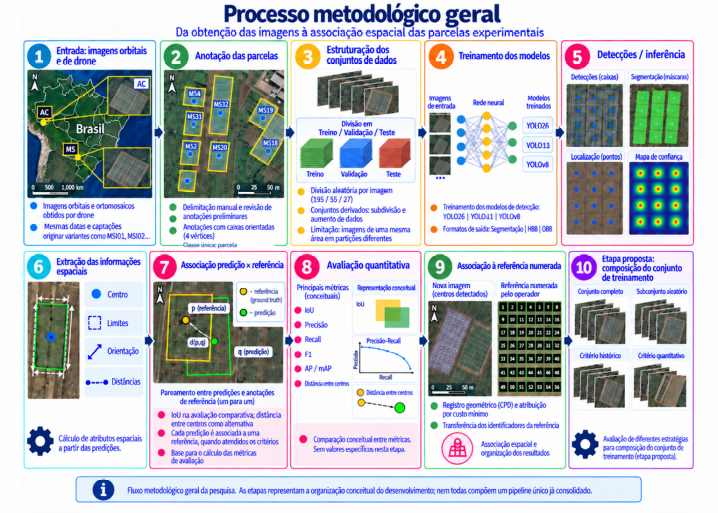
\includegraphics[width=0.95\textwidth]{figuras/figura13.png}
  \caption{Processo metodol\'ogico geral da pesquisa.}
  \label{fig:processo-metodologico}
  \fonte{Elaborado pelo autor (2026).}
\end{figure}

A sequ\^encia descreve a organiza\c{c}\~ao da pesquisa, e n\~ao um fluxo integrado. A detec\c{c}\~ao e a extra\c{c}\~ao das posi\c{c}\~oes foram implementadas, assim como a rotina que associa as detec\c{c}\~oes de novas imagens a uma refer\^encia previamente numerada. Essa rotina usa registro geom\'etrico e atribui\c{c}\~ao entre objetos; ela n\~ao l\^e um arquivo de croqui e ainda n\~ao identifica posi\c{c}\~oes experimentais que ficaram sem detec\c{c}\~ao.

\section{Origem e organiza\c{c}\~ao das imagens}
\label{sec:origem-organizacao-imagens}

As imagens orbitais foram obtidas no \textit{Google Earth}, em sua maioria por captura de tela, e re\'unem diferentes \'areas experimentais e, em alguns casos, a mesma \'area em datas distintas do hist\'orico de imagens. Os ortomosaicos foram gerados a partir de imagens obtidas por drone em campos experimentais da Embrapa Gado de Corte e incorporados ao conjunto de dados.

Quando uma \'area aparece em mais de uma data, mant\'em-se o identificador do campo e acrescenta-se um \'indice \`a varia\c{c}\~ao temporal (por exemplo, \textit{MS10-1} e \textit{MS10-2}), de modo que as imagens permane\c{c}am associadas ao mesmo campo.

Parte dos arquivos traz no nome a data e a hora da captura de tela, que n\~ao correspondem \`a data de aquisi\c{c}\~ao da imagem. A Figura~\ref{fig:organizacao-anual} exemplifica a organiza\c{c}\~ao anual das imagens hist\'oricas de uma mesma \'area.

\begin{figure}[htb]
  \centering
  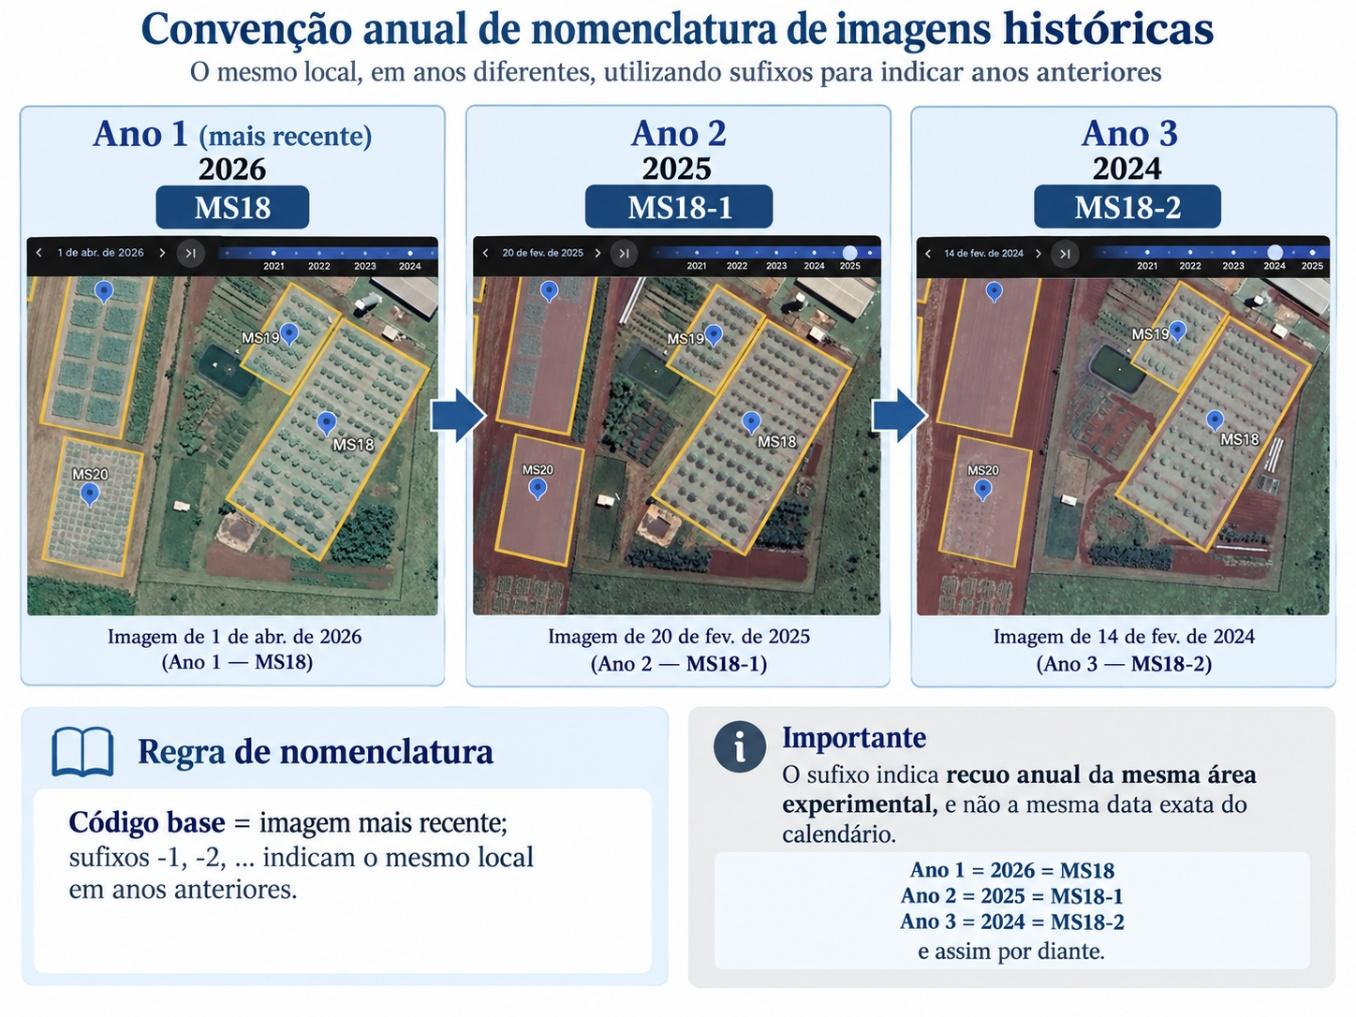
\includegraphics[width=0.95\textwidth]{figuras/figura14.jpg}
  \caption{Organiza\c{c}\~ao anual das imagens hist\'oricas de uma mesma \'area experimental.}
  \label{fig:organizacao-anual}
  \fonte{Elaborado pelo autor (2026).}
\end{figure}

\section{Evolu\c{c}\~ao e organiza\c{c}\~ao dos conjuntos de dados}
\label{sec:evolucao-conjuntos-dados}

O acervo anotado foi constru\'ido em quatro coletas. A primeira reuniu uma imagem orbital por campo experimental, de uma mesma data, e resultou em 35 imagens e 3.444 parcelas. A segunda cobriu 16 campos em diferentes datas do hist\'orico do \textit{Google Earth}, com 54 imagens e 8.179 parcelas anotadas por pol\'igonos. A terceira acrescentou ortomosaicos obtidos por drone, e a quarta, em andamento, abrange 1.045 campos experimentais marcados no \textit{Google Earth}. O conjunto usado nos experimentos mais recentes tem 277 imagens, 156 orbitais e 121 de drone, e 51.245 parcelas anotadas por quatro v\'ertices, isto \'e, como caixas orientadas. Nenhuma imagem da primeira coleta faz parte desse conjunto, enquanto todas as imagens da organiza\c{c}\~ao usada na localiza\c{c}\~ao por pontos est\~ao nele.

Nas primeiras coletas, as anota\c{c}\~oes foram feitas manualmente na plataforma Roboflow. Na terceira coleta, e tamb\'em na quarta, em andamento, adota-se um procedimento \textit{human-in-the-loop}: um modelo j\'a treinado gera anota\c{c}\~oes preliminares, que s\~ao conferidas e, quando necess\'ario, corrigidas manualmente. Trata-se de um procedimento de trabalho, e n\~ao de um m\'odulo do sistema.

As parcelas foram anotadas em uma \'unica classe, parcela, sem categorias para posi\c{c}\~oes vazias ou parcelas mortas. O conjunto de 277 imagens foi exportado da plataforma de anota\c{c}\~ao em abril de 2026, sem aumento de dados, e dividido aleatoriamente por imagem em 195 imagens de treinamento, 55 de valida\c{c}\~ao e 27 de teste. A parti\c{c}\~ao de teste, usada na avalia\c{c}\~ao comparativa dos detectores (Se\c{c}\~ao~\ref{sec:avaliacao-comparativa}), tem 7.852 parcelas; 12 de suas imagens s\~ao de drone e re\'unem 6.667 dessas parcelas.

Dois conjuntos derivados foram gerados a partir desse conjunto pelos procedimentos de prepara\c{c}\~ao descritos adiante. A subdivis\~ao das imagens densas resultou em 384 imagens (258 de treinamento, 80 de valida\c{c}\~ao e 46 de teste), com cada recorte mantido na parti\c{c}\~ao da imagem de origem. O segundo conjunto acrescenta vers\~oes transformadas ao treinamento, que passa a ter 3.406 imagens, e mant\'em a valida\c{c}\~ao e o teste do conjunto subdividido (80 e 46 imagens). O arquivo descritor desse segundo conjunto, contudo, aponta para os diret\'orios do conjunto subdividido; por isso, o treinamento do \textit{YOLO26m} realizado em agosto de 2026, que registra esse descritor, utilizou 258 imagens de treinamento sem as vers\~oes transformadas.

Os 1.045 campos da quarta coleta foram marcados no \textit{Google Earth}, e suas imagens orbitais s\~ao obtidas a partir dessas coordenadas com a biblioteca \textit{leafmap}, uma por campo. Com os novos ortomosaicos obtidos por drone, o acervo deve ultrapassar 1.200 imagens de campo. Essas imagens ainda n\~ao fazem parte dos conjuntos anotados usados nos experimentos apresentados neste trabalho. A Tabela~\ref{tab:conjuntos-dados} re\'une a composi\c{c}\~ao e o uso de cada conjunto.

\begin{table}[htb]
\centering
\caption{Conjuntos de dados do projeto}
\label{tab:conjuntos-dados}
\small
\begin{tabular}{p{3.3cm}p{5.7cm}p{5.7cm}}
\hline
\textbf{Conjunto} & \textbf{Composi\c{c}\~ao} & \textbf{Uso no projeto} \\
\hline
Primeira coleta & 35 imagens e 3.444 parcelas; 26 de treinamento, 6 de valida\c{c}\~ao e 3 de teste & Constru\c{c}\~ao inicial do acervo \\
Segunda coleta & 54 imagens e 8.179 parcelas; 39 de treinamento, 10 de valida\c{c}\~ao e 5 de teste; anota\c{c}\~oes poligonais & Amplia\c{c}\~ao do acervo anotado \\
Organiza\c{c}\~ao para localiza\c{c}\~ao por pontos & 54 imagens; 46 de treinamento, 5 de valida\c{c}\~ao e 3 de teste; anota\c{c}\~oes pontuais & Linha de localiza\c{c}\~ao por mapas de confian\c{c}a \\
Conjunto de 277 imagens (dataset6-OBB) & 277 imagens (156 orbitais e 121 de drone) e 51.245 parcelas; 195 de treinamento, 55 de valida\c{c}\~ao e 27 de teste; caixas orientadas & Parti\c{c}\~ao de teste (27 imagens, 7.852 parcelas) usada na avalia\c{c}\~ao comparativa; origem dos conjuntos derivados \\
Conjunto subdividido (dataset\_imgs\_split) & 384 imagens; 258 de treinamento, 80 de valida\c{c}\~ao e 46 de teste & Treinamento do YOLO26m (agosto de 2026) \\
Conjunto com aumento pr\'evio (dataset\_imgs\_aug) & 3.532 imagens; 3.406 de treinamento, 80 de valida\c{c}\~ao e 46 de teste & Caixas orientadas de maio e agosto de 2026 \\
Coleta por coordenadas & 1.045 campos, uma imagem orbital por campo; com os novos ortomosaicos de drone, mais de 1.200 imagens & Ainda n\~ao utilizada nos experimentos apresentados \\
\hline
\end{tabular}
\end{table}

\section{Depend\^encia entre imagens nas parti\c{c}\~oes}
\label{sec:dependencia-imagens-particoes}

No conjunto de 277 imagens, a divis\~ao aleat\'oria por imagem colocou em parti\c{c}\~oes diferentes imagens de uma mesma \'area. As imagens do quadrante Q5, obtidas em seis datas, est\~ao nas tr\^es parti\c{c}\~oes: quatro no treinamento, uma na valida\c{c}\~ao e uma no teste. As imagens identificadas como quadrante 12 tamb\'em aparecem nas tr\^es parti\c{c}\~oes, e as dos quadrantes Q4 e 15, no treinamento e na valida\c{c}\~ao. A organiza\c{c}\~ao de 54 imagens usada na localiza\c{c}\~ao por pontos apresenta a mesma situa\c{c}\~ao.

H\'a tamb\'em recortes de uma mesma captura de tela em parti\c{c}\~oes diferentes. Em duas capturas, recortes distintos foram para o treinamento e para o teste; em uma delas, o recorte do treinamento est\'a quase inteiramente contido no recorte do teste. Em uma terceira captura, os recortes ficaram no treinamento e na valida\c{c}\~ao. Al\'em disso, v\'arias capturas foram feitas em sequ\^encia, com poucos segundos de intervalo, e distribu\'idas entre parti\c{c}\~oes, de modo que parte delas pode cobrir \'areas iguais ou adjacentes.

Com essa organiza\c{c}\~ao, parte das imagens de valida\c{c}\~ao e de teste est\'a espacialmente relacionada a imagens de treinamento. Isso n\~ao implica que o modelo tenha memorizado os campos nem que uma m\'etrica espec\'ifica esteja incorreta, mas reduz a independ\^encia entre treinamento e avalia\c{c}\~ao e limita a leitura das m\'etricas como estimativa de generaliza\c{c}\~ao para \'areas n\~ao vistas \citep{kattenborn2022}. Os resultados da avalia\c{c}\~ao comparativa foram obtidos com essa parti\c{c}\~ao e s\~ao interpretados com essa restri\c{c}\~ao. Nenhuma nova divis\~ao foi criada para substitu\'i-la retrospectivamente.

A prepara\c{c}\~ao dos dados compreende convers\~ao de formato, redimensionamento, subdivis\~ao das imagens e aumento pr\'evio de dados, executados por scripts independentes do fluxo principal, al\'em das transforma\c{c}\~oes aplicadas pela biblioteca durante o treinamento. Um utilit\'ario converte arquivos \textit{TIFF} em imagens \textit{JPEG}, em RGB e com qualidade 90. A convers\~ao aplica compress\~ao com perdas e n\~ao transfere as informa\c{c}\~oes de georreferenciamento dos arquivos \textit{GeoTIFF} obtidos na coleta por coordenadas.

Imagens com largura inferior a 1.024 \textit{pixels} s\~ao ampliadas por interpola\c{c}\~ao bic\'ubica, com preserva\c{c}\~ao da propor\c{c}\~ao; as demais n\~ao s\~ao alteradas. A amplia\c{c}\~ao aumenta as dimens\~oes das parcelas em pixels, mas n\~ao recupera detalhe ausente da imagem original. A subdivis\~ao foi adotada para limitar o n\'umero de objetos por amostra nas imagens muito densas, de modo que cada recorte tenha, em geral, at\'e cerca de 500 parcelas.

Ap\'os o redimensionamento, imagens com 101 a 500 objetos s\~ao gravadas inteiras. As demais s\~ao percorridas por uma grade de recortes de 1.024 \textit{pixels}, com recortes menores nas bordas. Em cada recorte, contam-se os objetos cujo centro est\'a dentro de seus limites; se a contagem passar de 500 e o recorte tiver mais de 384 \textit{pixels} nas duas dimens\~oes, ele \'e dividido em quatro quadrantes, e o procedimento se repete em cada um. Caso contr\'ario, o recorte \'e gravado.

Com esse crit\'erio, um recorte que j\'a n\~ao pode ser dividido \'e gravado mesmo com mais de 500 objetos, e recortes com menos de 101 objetos tamb\'em s\~ao gravados. A faixa de 101 a 500 objetos \'e o intervalo visado, e n\~ao uma propriedade de todos os recortes.

\subsection{Tratamento das anota\c{c}\~oes nos recortes}
\label{sec:tratamento-anotacoes-recortes}

As coordenadas das anota\c{c}\~oes, originalmente normalizadas em rela\c{c}\~ao \`a imagem inteira, s\~ao convertidas para \textit{pixels}, ajustadas ao sistema de coordenadas do recorte e re-normalizadas em rela\c{c}\~ao \`as suas dimens\~oes. Cada anota\c{c}\~ao \'e atribu\'ida a um recorte pela posi\c{c}\~ao de seu centro, calculado como a m\'edia dos v\'ertices. Uma parcela que intersecta o recorte, mas cujo centro est\'a fora dele, n\~ao \'e inclu\'ida.

Anota\c{c}\~oes poligonais s\~ao recortadas nas bordas e descartadas se ficarem com menos de tr\^es v\'ertices ou com \'area inferior a 4 \textit{pixels} quadrados. Caixas s\~ao reduzidas \`a interse\c{c}\~ao com o recorte e descartadas quando essa interse\c{c}\~ao \'e degenerada ou quando o centro da caixa resultante fica fora do recorte. O procedimento evita anota\c{c}\~oes degeneradas nas bordas, mas uma parcela truncada pode n\~ao representar adequadamente a parcela original.

Um segundo script gera vers\~oes transformadas das imagens e das anota\c{c}\~oes, com rota\c{c}\~ao, cisalhamento, varia\c{c}\~ao de escala, distor\c{c}\~ao de perspectiva e varia\c{c}\~ao de contraste. Na configura\c{c}\~ao do script, cada imagem gera doze variantes, com \^angulos de 0\textdegree{} a 330\textdegree{} em passos de 30\textdegree{}, e a imagem original \'e copiada para o conjunto derivado. Os demais par\^ametros s\~ao sorteados nos intervalos de -15\textdegree{} a 15\textdegree{} (cisalhamento), 0,5 a 1,5 (escala), at\'e 0,05 (perspectiva) e 0,5 a 1,75 (contraste). A supress\~ao de regi\~oes da imagem est\'a implementada, mas desativada.

O sorteio usa um gerador pseudoaleat\'orio com semente 42, o que n\~ao garante, sozinho, a reprodu\c{c}\~ao exata das imagens transformadas, que depende tamb\'em da biblioteca e da ordem de processamento. Para transformar as anota\c{c}\~oes, cada parcela \'e rasterizada em uma m\'ascara pr\'opria, e todas as m\'ascaras recebem a mesma transforma\c{c}\~ao geom\'etrica aplicada \`a imagem. Os contornos externos s\~ao ent\~ao extra\'idos m\'ascara a m\'ascara, o que evita que parcelas vizinhas que passem a se tocar ap\'os a transforma\c{c}\~ao sejam reconstru\'idas como um \'unico objeto.

Os r\'otulos resultantes s\~ao pol\'igonos com n\'umero vari\'avel de v\'ertices, e o procedimento n\~ao garante a conserva\c{c}\~ao de todas as inst\^ancias originais. As imagens geradas derivam das mesmas imagens de origem e n\~ao constituem observa\c{c}\~oes independentes.

\subsection{Transforma\c{c}\~oes durante o treinamento}
\label{sec:transformacoes-treinamento}

A configura\c{c}\~ao de treinamento tamb\'em define transforma\c{c}\~oes aplicadas pela biblioteca no carregamento das amostras, como composi\c{c}\~ao em mosaico, mistura de imagens, altera\c{c}\~oes geom\'etricas e ajustes de cor, segundo as probabilidades e condi\c{c}\~oes da pr\'opria biblioteca. Os valores da configura\c{c}\~ao atual n\~ao estabelecem os que foram usados nos treinamentos anteriores. O conjunto com aumento pr\'evio cont\'em vers\~oes transformadas apenas no treinamento, enquanto a vers\~ao atual do script processa somente os subconjuntos de valida\c{c}\~ao.

O script de prepara\c{c}\~ao processa separadamente treinamento, valida\c{c}\~ao e teste e grava as sa\'idas nas parti\c{c}\~oes correspondentes, de modo que cada recorte permanece na parti\c{c}\~ao de sua imagem de origem. Isso n\~ao elimina a depend\^encia descrita em ``Depend\^encia entre imagens nas parti\c{c}\~oes''. N\~ao h\'a resultados de compara\c{c}\~oes controladas que isolem o efeito do redimensionamento, da subdivis\~ao ou do aumento de dados sobre o desempenho.

\section{Abordagens de vis\~ao computacional investigadas}
\label{sec:abordagens-investigadas}

As formas investigadas para identificar e localizar as parcelas diferem pela representa\c{c}\~ao de sa\'ida. A segmenta\c{c}\~ao de inst\^ancias delimita cada parcela por m\'ascara ou contorno \citep{he2017}; a detec\c{c}\~ao por caixas horizontais representa cada parcela por um ret\^angulo alinhado aos eixos da imagem, como na formula\c{c}\~ao original da fam\'ilia \textit{YOLO} \citep{redmon2016}; a detec\c{c}\~ao por caixas orientadas acrescenta a esse ret\^angulo um \^angulo \citep{ding2019}; e a localiza\c{c}\~ao por mapas de confian\c{c}a produz uma resposta cont\'inua cujos m\'aximos indicam as posi\c{c}\~oes das parcelas \citep{arruda2022}. Tamb\'em foram treinados um detector em cascata e um classificador auxiliar, este sem fun\c{c}\~ao de localiza\c{c}\~ao.

A representa\c{c}\~ao de sa\'ida n\~ao se confunde com a gera\c{c}\~ao da fam\'ilia \textit{YOLO} nem com o tamanho do modelo: diferentes gera\c{c}\~oes foram usadas, e uma mesma gera\c{c}\~ao foi treinada com representa\c{c}\~oes diferentes. As linhas investigadas t\^em n\'iveis distintos de maturidade e n\~ao foram conduzidas sob um mesmo protocolo. Os checkpoints \textit{YOLO} de segmenta\c{c}\~ao, caixas horizontais e caixas orientadas foram avaliados sobre um conjunto de teste comum (Se\c{c}\~ao~\ref{sec:avaliacao-comparativa}). A localiza\c{c}\~ao por mapas de confian\c{c}a e a detec\c{c}\~ao em cascata n\~ao fazem parte dessa avalia\c{c}\~ao.

A segmenta\c{c}\~ao de inst\^ancias foi uma das primeiras linhas investigadas. O modelo recebe a imagem e produz uma m\'ascara para cada parcela identificada, com treinamento supervisionado pelas anota\c{c}\~oes poligonais. Foram usadas as gera\c{c}\~oes \textit{YOLOv8, YOLO11 e YOLO26} \citep{jocher2026}, por meio da biblioteca \textit{Ultralytics} \citep{jocher2023}. Esses modelos foram treinados em momentos distintos, com diferen\c{c}as de tamanho de entrada, tamanho de lote, n\'umero de \'epocas e demais configura\c{c}\~oes, de modo que seus resultados n\~ao constituem uma compara\c{c}\~ao controlada entre gera\c{c}\~oes.

Na detec\c{c}\~ao por caixas horizontais, cada parcela \'e representada por uma caixa alinhada aos eixos da imagem. O interesse est\'a na presen\c{c}a e na posi\c{c}\~ao da parcela, sem delimitar o contorno da vegeta\c{c}\~ao, e o centro da caixa \'e obtido diretamente, o que simplifica a localiza\c{c}\~ao e a ordena\c{c}\~ao espacial.

A detec\c{c}\~ao por caixas orientadas representa cada parcela por um ret\^angulo acrescido de um par\^ametro de orienta\c{c}\~ao, de modo que a predi\c{c}\~ao \'e descrita por posi\c{c}\~ao, dimens\~oes e \^angulo. Essa formula\c{c}\~ao permite descrever objetos cuja dire\c{c}\~ao predominante n\~ao coincide com os eixos horizontal e vertical da imagem, condi\c{c}\~ao frequente em imagens a\'ereas \citep{ding2019,ding2022}. Em um contexto especificamente agr\'icola, \citet{zhang2025} avaliam uma rede de segmenta\c{c}\~ao orientada voltada \`a extra\c{c}\~ao de parcelas de melhoramento rotacionadas em imagens RGB de VANT, tratando a orienta\c{c}\~ao como parte expl\'icita da representa\c{c}\~ao.

A orienta\c{c}\~ao passou a ser tratada explicitamente para lidar com imagens nas quais as parcelas aparecem rotacionadas em rela\c{c}\~ao aos eixos. Na primeira coleta, a rota\c{c}\~ao era corrigida antes da captura das imagens, e as parcelas eram anotadas com caixas sem inclina\c{c}\~ao. Duas alternativas foram consideradas: ampliar o conjunto com rota\c{c}\~oes das mesmas imagens, com risco de sobreajuste, ou adotar uma representa\c{c}\~ao que aprendesse a orienta\c{c}\~ao, o que acrescenta um par\^ametro angular \`a caixa. A segunda levou aos modelos de caixas orientadas, e o aumento pr\'evio com rota\c{c}\~oes tamb\'em foi implementado. A delimita\c{c}\~ao exata do contorno, obtida pela segmenta\c{c}\~ao, foi considerada desnecess\'aria para a fenotipagem realizada na Embrapa Gado de Corte, o que justificou o uso de caixas nessa aplica\c{c}\~ao. Os checkpoints de caixas orientadas s\~ao os mais recentes do projeto, e um deles, \textbf{260525\_2231}, \'e o modelo indicado na configura\c{c}\~ao do sistema para infer\^encia.

Checkpoints das tr\^es representa\c{c}\~oes foram avaliados sobre o mesmo conjunto de teste, mas essa avalia\c{c}\~ao n\~ao \'e uma abla\c{c}\~ao da representa\c{c}\~ao geom\'etrica: os treinamentos ocorreram em etapas diferentes, com configura\c{c}\~oes e conjuntos de treinamento distintos. Diferen\c{c}as de desempenho n\~ao podem, portanto, ser atribu\'idas apenas \`a orienta\c{c}\~ao das caixas.

\section{Localiza\c{c}\~ao por mapas de confian\c{c}a}
\label{sec:localizacao-mapas-confianca}

Uma linha metodol\'ogica distinta, motivada por \citet{arruda2022} e fundamentada na Se\c{c}\~ao~\ref{sec:multistagerefinementnet}, representa as parcelas por mapas de confian\c{c}a em vez de caixas ou m\'ascaras. A sa\'ida da rede \'e um mapa cont\'inuo, e n\~ao uma lista de coordenadas: as posi\c{c}\~oes s\~ao obtidas em p\'os-processamento, pela identifica\c{c}\~ao de m\'aximos locais, e o resultado \'e um conjunto de pontos, sem delimita\c{c}\~ao da extens\~ao de cada parcela. A implementa\c{c}\~ao do projeto, em \textit{TensorFlow} e \textit{Keras}, \'e descrita na subse\c{c}\~ao~\ref{sec:implementacao-mapas-confianca}.

Tamb\'em foi treinado um detector Cascade R-CNN, arquitetura que encadeia est\'agios de detec\c{c}\~ao com limiares de correspond\^encia progressivamente mais estritos \citep{cai2018}, implementado com a biblioteca \textit{MMDetection} e \textit{backbone ResNet-50} \citep{he2016} com FPN \citep{lin2017}. Houve duas execu\c{c}\~oes de 12 \'epocas, com valida\c{c}\~ao ao fim de cada \'epoca, que leram diret\'orios de dados diferentes, cuja equival\^encia n\~ao foi verificada. A linha foi descontinuada antes de uma avalia\c{c}\~ao no conjunto de teste; seus resultados s\~ao apresentados na Se\c{c}\~ao~\ref{sec:linhas-paralelas}.

O classificador auxiliar n\~ao localiza parcelas: classifica cada imagem conforme a dificuldade que ela representa para o detector, a partir de r\'otulos avaliados, sua constru\c{c}\~ao, treinamento e limita\c{c}\~oes s\~ao descritos na subse\c{c}\~ao~\ref{sec:classificador-auxiliar-efficientnet}, ``Classificador auxiliar de dificuldade baseado em EfficientNet-B0''.

\section{Propostas estruturais investigadas para a associa\c{c}\~ao ao croqui}
\label{sec:propostas-estruturais}

Al\'em das abordagens visuais, duas propostas estruturais, \textit{Grid Completion} e \textit{Loss de Matriz}, foram formuladas para relacionar as detec\c{c}\~oes \`a organiza\c{c}\~ao espacial esperada do experimento; ambas s\~ao descritas na subse\c{c}\~ao~\ref{sec:propostas-anteriores-organizacao}, ``Propostas anteriores relacionadas \`a organiza\c{c}\~ao espacial''. A Tabela~\ref{tab:abordagens-papel} re\'une o papel e o estado documentado de cada componente investigado.

\begin{table}[htb]
\centering
\caption{Abordagens visuais, classifica\c{c}\~ao auxiliar e propostas estruturais: papel e estado documentado}
\label{tab:abordagens-papel}
\small
\begin{tabular}{p{4cm}p{4.3cm}p{6.4cm}}
\hline
\textbf{Abordagem ou componente} & \textbf{Representa\c{c}\~ao de sa\'ida} & \textbf{Fun\c{c}\~ao no projeto} \\
\hline
Segmenta\c{c}\~ao de inst\^ancias (YOLOv8, YOLO11, YOLO26) & M\'ascara ou contorno por parcela & Linha inicial de identifica\c{c}\~ao \\
Detec\c{c}\~ao por caixas horizontais (YOLO26) & Ret\^angulo alinhado aos eixos & Representa\c{c}\~ao intermedi\'aria; base geom\'etrica para extra\c{c}\~ao de centros \\
Detec\c{c}\~ao por caixas orientadas (YOLO26) & Ret\^angulo com par\^ametro de orienta\c{c}\~ao & Representa\c{c}\~ao do modelo indicado para infer\^encia \\
Localiza\c{c}\~ao por mapas de confian\c{c}a & Mapa cont\'inuo; posi\c{c}\~oes obtidas por m\'aximos locais no p\'os-processamento & Linha alternativa de localiza\c{c}\~ao e contagem, sem avalia\c{c}\~ao quantitativa \\
Detec\c{c}\~ao em cascata (Cascade R-CNN) & Caixas & Linha descontinuada antes da avalia\c{c}\~ao no conjunto de teste \\
Classificador auxiliar (EfficientNet-B0) & Classe bin\'aria por imagem & Classifica\c{c}\~ao da dificuldade operacional em rela\c{c}\~ao ao detector \\
Grid Completion (proposta estrutural) & Grade te\'orica e c\'elulas sem detec\c{c}\~ao & Implementada em 2025 e removida do c\'odigo em 2026 \\
\hline
\end{tabular}
\end{table}

Os \textit{checkpoints} preservados documentam execu\c{c}\~oes de treinamento feitas ao longo do desenvolvimento, em uma trajet\'oria incremental, e n\~ao um estudo comparativo planejado desde o in\'icio. S\~ao dezesseis \textit{checkpoints} treinados; a Tabela~\ref{tab:experimentos-yolo} apresenta seis deles, um para cada combina\c{c}\~ao principal de gera\c{c}\~ao, tamanho de modelo e representa\c{c}\~ao de sa\'ida. A caracteriza\c{c}\~ao dos treinamentos usa os metadados gravados nos pr\'oprios \textit{checkpoints}: par\^ametros de configura\c{c}\~ao, caminhos dos descritores de dados e hist\'oricos por \'epoca.

O treinamento parte de um \textit{checkpoint} indicado na configura\c{c}\~ao como modelo-base e do descritor do conjunto de dados, e \'e interrompido se algum deles n\~ao estiver dispon\'ivel. Os par\^ametros da configura\c{c}\~ao, o caminho do conjunto de dados e a identifica\c{c}\~ao da execu\c{c}\~ao s\~ao encaminhados \`a biblioteca \textit{Ultralytics}, que conduz o ajuste do modelo. A configura\c{c}\~ao tamb\'em permite retomar uma execu\c{c}\~ao interrompida.

Ao fim de uma execu\c{c}\~ao, o sistema copia o arquivo de melhores pesos com um nome padronizado, formado pelo carimbo de data e hora de modifica\c{c}\~ao do arquivo, pelo nome do modelo-base, por uma identifica\c{c}\~ao de t\'ecnica e pelo mAP@0,5 de valida\c{c}\~ao obtido ao final do treinamento. No treinamento do \textit{YOLO26m} de agosto de 2026, o carimbo \textbf{260810\_2042} coincide com o t\'ermino da execu\c{c}\~ao, e o sufixo \textbf{96\_2} \'e compat\'ivel com o maior \textbf{mAP@0,5} de valida\c{c}\~ao registrado, \textbf{0,96253}, na \'epoca 90. A escolha dos melhores pesos segue o crit\'erio da biblioteca. Os nomes dos \textit{checkpoints} anteriores n\~ao seguem integralmente essa regra e, por isso, n\~ao s\~ao usados para reconstruir sua origem.

\subsection{Procedimentos de valida\c{c}\~ao nos experimentos hist\'oricos}
\label{sec:procedimentos-validacao-historicos}

Parte dos \textit{checkpoints} traz no nome termos de valida\c{c}\~ao cruzada (\textit{leave-one-out} e valida\c{c}\~ao aninhada), e os caminhos de sess\~ao gravados nos metadados confirmam essa organiza\c{c}\~ao. Na sess\~ao \textit{\textbf{nested}\_cv\_20260318\_162914}, os checkpoints \textbf{260318\_2058} e \textbf{260320\_0320} registram as parti\c{c}\~oes externas \textit{outer\_fold\_1} e \textit{outer\_fold\_5}, com limite de 60 \'epocas, e o checkpoint \textbf{260323\_1718}, associado ao diret\'orio \textit{final\_model} da mesma sess\~ao, registra 120 \'epocas.

Os resultados das demais parti\c{c}\~oes e os resultados agregados dessas valida\c{c}\~oes n\~ao est\~ao dispon\'iveis. Um modelo identificado como final n\~ao \'e um resultado agregado de valida\c{c}\~ao cruzada, e o limite de \'epocas registrado para ele n\~ao se aplica \`as parti\c{c}\~oes.

A Tabela~\ref{tab:experimentos-yolo} re\'une os par\^ametros das seis execu\c{c}\~oes, recuperados dos metadados de cada checkpoint. Todas usam o otimizador \textbf{AdamW} \citep{loshchilov2019} e diferem em taxa inicial de aprendizagem, paci\^encia, tamanho de lote e dimens\~ao de entrada; as vers\~oes declaradas da biblioteca e as ra\'izes dos caminhos de arquivos tamb\'em variam entre elas.

\begin{table}[htb]
\centering
\caption{Experimentos com modelos da fam\'ilia YOLO}
\label{tab:experimentos-yolo}
\small
\begin{tabular}{p{1.7cm}p{3.4cm}p{4.2cm}p{1.7cm}p{1cm}p{1.2cm}}
\hline
\textbf{ID} & \textbf{Modelo e tarefa} & \textbf{Evid\^encia do protocolo} & \textbf{\'Epocas config.} & \textbf{Lote} & \textbf{imgsz} \\
\hline
EXP-002 & YOLOv8n, segmenta\c{c}\~ao & \textit{Leave-one-out} (nome e caminho da sess\~ao) & 100 & 8 & 640 \\
EXP-003 & YOLO11n, segmenta\c{c}\~ao & \textit{Leave-one-out} (nome e caminho da sess\~ao) & 100 & 16 & 640 \\
EXP-006 & YOLO26s, segmenta\c{c}\~ao & Valida\c{c}\~ao aninhada, modelo final (caminho da sess\~ao) & 120 & 8 & 1024 \\
EXP-009 & YOLO26s, caixas horizontais & Valida\c{c}\~ao aninhada, modelo final (caminho da sess\~ao) & 120 & 4 & 1024 \\
EXP-013 & YOLO26s, caixas orientadas & Sem valida\c{c}\~ao cruzada & 120 & 8 & 1024 \\
EXP-016 & YOLO26m, caixas orientadas & Sem valida\c{c}\~ao cruzada & 120 & 8 & 1280 \\
\hline
\end{tabular}

\vspace{0.3cm}
\footnotesize \textit{Nota: \'epocas, lote e imgsz (dimens\~ao de entrada, em pixels) foram recuperados dos metadados de configura\c{c}\~ao de cada checkpoint; nas seis execu\c{c}\~oes, o hist\'orico por \'epoca chega ao limite configurado. Os demais par\^ametros, como taxa inicial de aprendizagem, paci\^encia e semente, tamb\'em constam desses metadados. O EXP-016 foi repetido com lote 8 depois que a primeira tentativa, com lote 12, falhou por falta de mem\'oria na GPU na \'epoca 18.}
\end{table}

\subsection{Proveni\^encia dos conjuntos de dados}
\label{sec:proveniencia-conjuntos}

Os metadados registram o caminho do descritor de dados de cada execu\c{c}\~ao. Parte dos \textit{checkpoints} de 2025 e do primeiro semestre de 2026 aponta para descritores de sess\~oes de valida\c{c}\~ao cruzada. Os \textit{checkpoints} \textbf{251004\_2132} e \textbf{251022\_1208} foram treinados com conjuntos ponderados por dificuldade: cada imagem recebeu manualmente um n\'ivel de 1 a 4, e as imagens foram replicadas no treinamento em n\'umero aproximadamente proporcional ao quadrado desse n\'ivel. Os checkpoints de caixas orientadas de maio de 2026 registram os diret\'orios \textit{dataset\_imgs\_aug1} (\textbf{260525\_2231}) e \textit{dataset\_imgs\_aug} (\textbf{260528\_0037} e \textbf{260530\_1336}), e o \textit{YOLO26m} de agosto registra \textit{dataset\_imgs\_aug}.

Os \textit{checkpoints} \textbf{260525\_2231} e \textbf{260530\_1336} ilustram esse limite: o primeiro registra dataset\_imgs\_aug1 e dimens\~ao de entrada de 1.024 pixels; o segundo, \textit{dataset\_imgs\_aug} e 1.280 pixels. As execu\c{c}\~oes diferem na configura\c{c}\~ao e possivelmente nos dados, e por isso a diferen\c{c}a de desempenho descrita nos Resultados n\~ao tem causa identificada.

\subsection{Alcance da compara\c{c}\~ao entre esses experimentos}
\label{sec:alcance-comparacao}

A avalia\c{c}\~ao comparativa aplicou 15 \textit{checkpoints} treinados e o modelo-base sem ajuste ao mesmo teste de 27 imagens, com os mesmos par\^ametros de infer\^encia e de correspond\^encia. Essa condi\c{c}\~ao comum permite comparar os modelos de forma descritiva, mas n\~ao equaliza o treinamento: os \textit{checkpoints} diferem em gera\c{c}\~ao, tamanho, representa\c{c}\~ao de sa\'ida, dimens\~ao de entrada, n\'umero de \'epocas, dados de treinamento e vers\~ao da biblioteca, e nenhuma dessas vari\'aveis foi isolada. \textit{Checkpoints} treinados com uma dimens\~ao de entrada e avaliados com outra podem, al\'em disso, ser afetados por essa diferen\c{c}a. O YOLO26m de agosto de 2026 foi avaliado depois, com dimens\~ao de entrada de 1.280 \textit{pixels} e uma vers\~ao posterior do script de avalia\c{c}\~ao, e seu resultado \'e apresentado \`a parte.

\subsection{Implementa\c{c}\~ao da abordagem baseada em mapas de confian\c{c}a}
\label{sec:implementacao-mapas-confianca}

A implementa\c{c}\~ao dessa abordagem trabalha com uma representa\c{c}\~ao diferente da usada pelos detectores. As posi\c{c}\~oes anotadas s\~ao convertidas em mapas de refer\^encia, amostrados em uma grade de pixels, que servem de alvo ao treinamento; as posi\c{c}\~oes das parcelas s\~ao estimadas depois, por p\'os-processamento.

A entrada dessa linha n\~ao s\~ao r\'otulos poligonais, mas pontos. Um utilit\'ario l\^e as anota\c{c}\~oes quadrilaterais (classe e oito coordenadas normalizadas), calcula a m\'edia dos quatro v\'ertices, converte o resultado para pixels e trunca os valores para inteiros. Cada arquivo passa a conter uma lista de posi\c{c}\~oes, sem classe e sem a extens\~ao da parcela.

No treinamento, a imagem \'e normalizada para o intervalo unit\'ario e redimensionada por interpola\c{c}\~ao bilinear at\'e a dimens\~ao de entrada da rede. As respostas de refer\^encia, por sua vez, s\~ao constru\'idas em uma resolu\c{c}\~ao menor que a da entrada, determinada por um fator de redu\c{c}\~ao. As coordenadas anotadas s\~ao reescaladas para essa resolu\c{c}\~ao por fatores calculados independentemente em cada eixo, a partir da raz\~ao entre as dimens\~oes do mapa e as da imagem original.

Sobre esse mapa, cada objeto produz uma resposta gaussiana bidimensional centrada em sua posi\c{c}\~ao. As respostas de objetos distintos s\~ao combinadas pelo m\'aximo ponto a ponto, e n\~ao por soma; assim, a soma do mapa n\~ao corresponde ao n\'umero de objetos, e objetos muito pr\'oximos podem n\~ao gerar picos distintos. Pontos que saem dos limites do mapa s\~ao descartados.

Cada est\'agio de refinamento tem seu pr\'oprio mapa de refer\^encia, constru\'ido com as mesmas anota\c{c}\~oes e com o desvio padr\~ao da gaussiana decrescendo linearmente entre um valor m\'aximo e um m\'inimo, conforme a motiva\c{c}\~ao do m\'etodo publicado: os est\'agios iniciais aprendem uma localiza\c{c}\~ao aproximada e os finais a refinam \citep{arruda2022}. Os desvios padr\~ao s\~ao ajustados pelo fator de redu\c{c}\~ao de resolu\c{c}\~ao, para que a dispers\~ao acompanhe a escala do mapa.

\subsubsection*{Organiza\c{c}\~ao da rede e op\c{c}\~oes configuradas}

A implementa\c{c}\~ao, denominada no c\'odigo do projeto como \textit{\textbf{MultiStageRefinementNet}}, segue a organiza\c{c}\~ao em tr\^es componentes descrita na Se\c{c}\~ao~\ref{sec:multistagerefinementnet}, com o m\'odulo de agrega\c{c}\~ao em pir\^amide configurado para quatro escalas e cada est\'agio de refinamento recebendo, al\'em da sa\'ida da agrega\c{c}\~ao, o mapa produzido pelo est\'agio anterior.

Os est\'agios n\~ao recebem a mesma entrada. O primeiro est\'agio recebe a sa\'ida do m\'odulo de agrega\c{c}\~ao em pir\^amide. Nos est\'agios seguintes, essa representa\c{c}\~ao \'e concatenada ao mapa de confian\c{c}a produzido pelo est\'agio anterior, permitindo o refinamento sucessivo das respostas. Cada est\'agio produz seu pr\'oprio mapa.

O extrator de caracter\'isticas pode ser a vers\~ao simplificada inspirada na VGG19, sem pr\'e-treino, ou a VGG19 pr\'e-treinada; a configura\c{c}\~ao padr\~ao seleciona a primeira, e um dos treinamentos usou a segunda. A entrada da rede tem 512 $\times$ 512 \textit{pixels}, a redu\c{c}\~ao de resolu\c{c}\~ao padr\~ao \'e de oito vezes, o que resulta em mapas de 64 $\times$ 64 \textit{pixels}, e h\'a quatro est\'agios de refinamento; um dos treinamentos usou redu\c{c}\~ao de quatro vezes.

\subsubsection*{Treinamento definido na implementa\c{c}\~ao}

A fun\c{c}\~ao de perda implementada \'e um erro quadr\'atico ponderado. Cada \textit{pixel} recebe um peso conforme o valor do mapa de refer\^encia naquela posi\c{c}\~ao: \textit{pixels} cujo alvo seja maior ou igual a um limiar recebem um peso maior, e os demais, um peso menor. O erro quadr\'atico ponderado \'e somado e dividido pela soma dos pesos, acrescida de uma pequena constante de estabiliza\c{c}\~ao, de modo que a perda corresponde a uma m\'edia ponderada e n\~ao a uma soma. O prop\'osito declarado no c\'odigo \'e compensar o desbalanceamento entre as regi\~oes de pico e o fundo do mapa, que ocupa a maior parte de sua \'area.

A classe de perda define, por padr\~ao, pesos 8 e 1 para as regi\~oes positivas e de fundo, com limiar de 0,05; o script de treinamento usa pesos 12 e 1 e limiar de 0,03.

Cada est\'agio \'e supervisionado pelo mapa de refer\^encia correspondente; as perdas dos est\'agios s\~ao somadas e divididas pelo n\'umero de imagens do lote. A publica\c{c}\~ao de refer\^encia define, em vez disso, uma soma de erros quadr\'aticos por posi\c{c}\~ao em cada est\'agio, somada entre est\'agios e sem pondera\c{c}\~ao entre regi\~oes \citep{arruda2022}.

A rede produz um mapa de confian\c{c}a por est\'agio. A localiza\c{c}\~ao utiliza o mapa do \'ultimo est\'agio, tanto na rotina de infer\^encia quanto na avalia\c{c}\~ao implementada. A obten\c{c}\~ao das posi\c{c}\~oes ocorre em uma etapa separada de p\'os-processamento, que identifica m\'aximos locais, aplica um limiar de confian\c{c}a e prev\^e supress\~ao opcional por dist\^ancia.

Um \textit{pixel} \'e candidato a m\'aximo local quando seu valor \'e igual ao maior valor de sua vizinhan\c{c}a ortogonal imediata, obtido por dilata\c{c}\~ao com n\'ucleo em cruz; diferentemente da compara\c{c}\~ao estrita da publica\c{c}\~ao de refer\^encia, esse crit\'erio aceita empates. Em seguida, ret\^em-se os candidatos com valor maior ou igual ao limiar de confian\c{c}a, e o script de execu\c{c}\~ao usa um limiar mais permissivo que o padr\~ao da fun\c{c}\~ao. A supress\~ao por dist\^ancia m\'inima, que descartaria candidatos pr\'oximos a outros de maior confian\c{c}a, est\'a fixada em um pixel e, portanto, n\~ao tem efeito.

A detec\c{c}\~ao de picos retorna inicialmente posi\c{c}\~oes na grade do mapa de confian\c{c}a. Em seguida, as coordenadas s\~ao reescaladas separadamente nos eixos horizontal e vertical para as dimens\~oes da imagem original e convertidas para valores inteiros. As posi\c{c}\~oes resultantes representam estimativas de localiza\c{c}\~ao nessa imagem, sem delimita\c{c}\~ao da extens\~ao das parcelas ou atribui\c{c}\~ao de identificadores do croqui. Sua correspond\^encia com parcelas efetivamente presentes dependeria de avalia\c{c}\~ao experimental.

O m\'odulo calcula, para a contagem, erro absoluto m\'edio, raiz do erro quadr\'atico m\'edio e coeficiente de determina\c{c}\~ao. Para a localiza\c{c}\~ao, cada refer\^encia \'e associada \`a primeira predi\c{c}\~ao ainda livre situada a at\'e quatro pixels de dist\^ancia, sem buscar a mais pr\'oxima nem fazer atribui\c{c}\~ao global. Esse crit\'erio difere da correspond\^encia por sobreposi\c{c}\~ao usada na avalia\c{c}\~ao dos detectores, e os valores dos dois protocolos n\~ao s\~ao diretamente compar\'aveis.

Modelos dessa linha foram treinados em diferentes configura\c{c}\~oes, e as m\'etricas de contagem (MAE, RMSE e R\textsuperscript{2}) e de localiza\c{c}\~ao (precis\~ao, recall e F1) foram calculadas no conjunto de valida\c{c}\~ao a cada \'epoca; os valores s\~ao apresentados nos Resultados.

A implementa\c{c}\~ao permanece em m\'odulo separado, sem integra\c{c}\~ao que use um modelo YOLO como extrator de caracter\'isticas.

\section{Classificador auxiliar de dificuldade baseado em \textit{EfficientNet-B0}}
\label{sec:classificador-auxiliar-efficientnet}

O classificador auxiliar estima, a partir da imagem, uma categoria de dificuldade em rela\c{c}\~ao ao detector usado para gerar seus r\'otulos. A sa\'ida n\~ao \'e uma propriedade agron\^omica da \'area, n\~ao identifica parcelas e n\~ao \'e uma medida geral de qualidade da imagem: indica apenas se se espera que o detector tenha desempenho elevado naquela imagem, segundo o crit\'erio descrito a seguir.

Os r\'otulos bin\'arios s\~ao obtidos automaticamente do F1 de cada imagem (coluna f1\_medio) em um arquivo de m\'etricas por imagem gerado em 7 de junho de 2026, com 4.992 registros.

Recebem classe 1 as imagens com F1 maior ou igual a 0,97, e classe 0 as demais. O limiar foi adotado empiricamente, sem deriva\c{c}\~ao estat\'istica, como par\^ametro para construir os r\'otulos; n\~ao \'e uma medida de acur\'acia da rede nem foi usado para selecionar imagens de treinamento do detector. Na data em que esses valores foram gerados, a configura\c{c}\~ao de detec\c{c}\~ao do sistema usava o \textit{checkpoint} 260525\_2231, com confian\c{c}a m\'inima de 0,3, entrada de 1.024 pixels e IoU de correspond\^encia de 0,3.

Os registros s\~ao divididos em 70\% para treinamento, 20\% para valida\c{c}\~ao e 10\% para teste, por duas divis\~oes sucessivas estratificadas pela classe e com semente fixa, sem agrupar previamente as vers\~oes derivadas de uma mesma imagem.

As imagens correspondentes s\~ao redimensionadas para 224 $\times$ 224 pixels por reamostragem LANCZOS, convertidas para RGB e gravadas em JPEG com qualidade 95 nos diret\'orios de cada subconjunto e classe. Registros sem arquivo de origem s\~ao contabilizados como ausentes.

O conjunto resultante tem 4.971 arquivos: 3.480 de treinamento, 994 de valida\c{c}\~ao e 497 de teste. A diferen\c{c}a em rela\c{c}\~ao aos 4.992 registros decorre de colis\~oes de nomes e de registros sem arquivo correspondente. Parte dos arquivos s\~ao vers\~oes transformadas de uma mesma imagem, produzidas antes da divis\~ao.

O m\'odulo tem um segundo diret\'orio de dados, \textit{dataset1}, cujas contagens coincidem com as que o mesmo arquivo de m\'etricas produz com limiar de F1 de 0,90 (4.343 imagens na classe 1). O c\'odigo preservado usa apenas o limiar de 0,97 e o diret\'orio dataset, ao qual corresponde a distribui\c{c}\~ao de classes do teste apresentada nos Resultados.

\subsection{Procedimento de treinamento}
\label{sec:procedimento-treinamento-classificador}

No carregamento, as imagens s\~ao redimensionadas para 224 $\times$ 224 \textit{pixels} e normalizadas com as estat\'isticas do pr\'e-treinamento. Apenas o treinamento recebe transforma\c{c}\~oes aleat\'orias (espelhamento horizontal, rota\c{c}\~ao de at\'e 20\textdegree{} e varia\c{c}\~ao de brilho e contraste); valida\c{c}\~ao e teste recebem s\'o redimensionamento e normaliza\c{c}\~ao. Isso n\~ao elimina as transforma\c{c}\~oes j\'a presentes nos arquivos antes da divis\~ao.

A rede \'e uma \textit{EfficientNet-B0} \citep{tan2019} inicializada com os pesos IMAGENET1K\_V1, pr\'e-treinados no \textit{ImageNet} \citep{deng2009}. A cabe\c{c}a de classifica\c{c}\~ao \'e substitu\'ida por camadas que reduzem a representa\c{c}\~ao de 1.280 para 256 dimens\~oes e depois para uma sa\'ida, com ativa\c{c}\~ao ReLU e dropout, e a perda \'e a BCEWithLogitsLoss.

O ajuste tem duas fases com o otimizador Adam \citep{kingma2015}: nas cinco primeiras \'epocas, o extrator pr\'e-treinado fica congelado e s\'o a nova cabe\c{c}a \'e otimizada, com taxa de aprendizagem de 1e-3; a partir da sexta, todos os par\^ametros s\~ao liberados e o otimizador \'e recriado com taxa de 1e-5.

A taxa de aprendizagem \'e reduzida por \textit{ReduceLROnPlateau} (fator 0,3, paci\^encia 3) quando a perda de valida\c{c}\~ao deixa de melhorar, e o treinamento \'e interrompido ap\'os sete \'epocas sem redu\c{c}\~ao da melhor perda de valida\c{c}\~ao, com m\'aximo de 50 \'epocas. Os pesos s\~ao salvos sempre que a perda de valida\c{c}\~ao atinge um novo m\'inimo.

O teste recria a arquitetura, carrega os pesos e classifica o subconjunto de teste: a sa\'ida passa pela fun\c{c}\~ao log\'istica, e a classe positiva \'e atribu\'ida quando o valor \'e maior ou igual a 0,5. O resultado \'e apresentado nos Resultados por matriz de confus\~ao e medidas por classe.

Dois arquivos de pesos est\~ao preservados no m\'odulo: efficientnet\_filtro\_qualidade.pth, cuja estrutura (362 tensores) corresponde \`a arquitetura descrita, e cnn\_filtro\_qualidade.pth, de uma arquitetura com 10 tensores.

\section{Depend\^encia entre os subconjuntos do classificador}
\label{sec:dependencia-subconjuntos-classificador}

A organiza\c{c}\~ao descrita tem duas limita\c{c}\~oes distintas.

A primeira \'e a depend\^encia entre vers\~oes transformadas de uma mesma imagem. A divis\~ao \'e feita por arquivo, sem considerar a imagem de origem, e derivados de uma mesma imagem podem ficar em subconjuntos diferentes. Agrupando os arquivos pela imagem de origem, identificada pela remo\c{c}\~ao do sufixo de aumento no nome, h\'a 383 imagens de origem, das quais 377 (98,4\%) t\^em derivados em mais de um subconjunto.

Com essa organiza\c{c}\~ao, o desempenho medido no teste n\~ao estima o desempenho em imagens de origem inteiramente novas. O efeito sobre as medidas n\~ao foi quantificado.

A segunda \'e a poss\'ivel sobreposi\c{c}\~ao entre as imagens usadas para gerar os r\'otulos e as imagens de treinamento do detector que produziu os valores de F1. Das 4.992 imagens avaliadas, 3.338 t\^em nomes de imagens de treinamento do conjunto com aumento pr\'evio, 79 de valida\c{c}\~ao e 46 de teste; as demais n\~ao est\~ao nos conjuntos atuais. Como os dados de treinamento do prov\'avel detector, o \textit{checkpoint} 260525\_2231, s\~ao indeterminados, a sobreposi\c{c}\~ao \'e prov\'avel, mas sua extens\~ao n\~ao pode ser medida.

O arquivo de m\'etricas do detector serve apenas para construir os r\'otulos; a rede recebe imagens, e n\~ao valores de F1. As predi\c{c}\~oes do classificador n\~ao s\~ao usadas para filtrar imagens, acionar treinamentos ou condicionar etapas do fluxo de detec\c{c}\~ao, e o componente permanece em m\'odulo pr\'oprio.

As sa\'idas dos detectores t\^em geometrias diferentes conforme a representa\c{c}\~ao, e as etapas posteriores operam sobre representa\c{c}\~oes mais simples. Esta subse\c{c}\~ao descreve como cada geometria \'e convertida em uma posi\c{c}\~ao pontual e quais representa\c{c}\~oes auxiliares s\~ao derivadas dessas posi\c{c}\~oes. Obter uma posi\c{c}\~ao pontual a partir de uma detec\c{c}\~ao \'e uma opera\c{c}\~ao puramente geom\'etrica: ela n\~ao estabelece se a detec\c{c}\~ao corresponde a uma parcela efetivamente presente, o que depende da compara\c{c}\~ao com anota\c{c}\~oes de refer\^encia, nem atribui a essa detec\c{c}\~ao o identificador da parcela no croqui, o que exige uma etapa pr\'opria de numera\c{c}\~ao ou de associa\c{c}\~ao \`a refer\^encia. Essas duas opera\c{c}\~oes s\~ao tratadas nas subse\c{c}\~oes seguintes.

\section{Representa\c{c}\~ao espacial das detec\c{c}\~oes}
\label{sec:representacao-espacial-deteccoes}

\subsection{Centros das detec\c{c}\~oes e centroides}
\label{sec:centros-deteccoes-centroides}

O sistema obt\'em posi\c{c}\~oes pontuais por caminhos distintos, conforme a representa\c{c}\~ao de sa\'ida e a rotina utilizada. O termo centroide, empregado de forma gen\'erica, encobre procedimentos que n\~ao s\~ao id\^enticos, ainda que possam produzir a mesma posi\c{c}\~ao em casos particulares.

No fluxo auxiliar que alimenta as estat\'isticas e as representa\c{c}\~oes derivadas, as predi\c{c}\~oes s\~ao primeiro reduzidas a caixas alinhadas aos eixos. Predi\c{c}\~oes j\'a produzidas nesse formato s\~ao lidas diretamente. Nesse caminho, quando est\~ao dispon\'iveis caixas associadas \`as sa\'idas de segmenta\c{c}\~ao, a posi\c{c}\~ao \'e calculada a partir dessas caixas, e n\~ao diretamente da distribui\c{c}\~ao dos \textit{pixels} da m\'ascara. Para predi\c{c}\~oes orientadas, havendo os quatro v\'ertices do quadril\'atero, a caixa alinhada aos eixos \'e obtida pelos extremos de suas coordenadas. H\'a tamb\'em um caminho alternativo que utiliza o centro, a largura e a altura fornecidos, sem incorporar o \^angulo \`a convers\~ao; esse caminho mant\'em o centro, mas n\~ao calcula, em geral, a mesma envolvente obtida a partir dos v\'ertices rotacionados. A posi\c{c}\~ao pontual \'e ent\~ao calculada como o ponto m\'edio entre os limites da caixa resultante.

No tra\c{c}ado das sa\'idas orientadas sobre a imagem, a posi\c{c}\~ao \'e obtida de outra forma: pela m\'edia aritm\'etica das coordenadas dos v\'ertices do quadril\'atero predito ou, quando a predi\c{c}\~ao \'e fornecida como centro, dimens\~oes e \^angulo, pelo centro informado pela pr\'opria representa\c{c}\~ao.

Para uma mesma caixa orientada retangular, antes de altera\c{c}\~oes geom\'etricas ou quantiza\c{c}\~ao, esses c\'alculos coincidem quanto \`a posi\c{c}\~ao central, embora preservem informa\c{c}\~oes diferentes sobre a extens\~ao e a orienta\c{c}\~ao. Essa equival\^encia decorre da simetria da representa\c{c}\~ao e n\~ao deve ser generalizada para pol\'igonos arbitr\'arios nem confundida com o centroide de \'area de uma regi\~ao segmentada.

Registra-se ainda que o procedimento de convers\~ao de anota\c{c}\~oes empregado na linha de localiza\c{c}\~ao por mapas de confian\c{c}a, descrito anteriormente, tamb\'em utiliza a m\'edia dos v\'ertices, por\'em a partir de coordenadas normalizadas e com convers\~ao final para inteiro.

Junto com as posi\c{c}\~oes, a mesma rotina calcula dimens\~oes m\'edias das detec\c{c}\~oes, obtidas como a m\'edia aritm\'etica das larguras e das alturas das caixas alinhadas aos eixos presentes naquela imagem. Esse valor \'e calculado por imagem, e n\~ao para o conjunto de dados como um todo, e serve de base para as representa\c{c}\~oes descritas a seguir.

As coordenadas resultantes s\~ao expressas em pixels da imagem processada, em valores reais, sem normaliza\c{c}\~ao. A convers\~ao para valores inteiros ocorre apenas nas opera\c{c}\~oes de tra\c{c}ado e de extra\c{c}\~ao de recortes. O sistema n\~ao realiza, nessa etapa, transforma\c{c}\~ao para coordenadas geogr\'aficas: as posi\c{c}\~oes permanecem no sistema de coordenadas da imagem.

\subsection{Caixas de tamanho uniforme}
\label{sec:caixas-tamanho-uniforme}

A partir das posi\c{c}\~oes pontuais e das dimens\~oes m\'edias calculadas para cada imagem, o sistema pode gerar caixas auxiliares de tamanho uniforme. As dimens\~oes nominais recebem a margem e os limites definidos no c\'odigo; cada caixa \'e centrada na posi\c{c}\~ao correspondente e recortada quando ultrapassa os limites da imagem.

Essa representa\c{c}\~ao \'e derivada das detec\c{c}\~oes e serve \`a visualiza\c{c}\~ao e aos recortes. N\~ao \'e uma nova predi\c{c}\~ao nem um refinamento da geometria original e, por ser alinhada aos eixos, n\~ao preserva a orienta\c{c}\~ao de uma caixa orientada. Nenhum resultado desta qualifica\c{c}\~ao depende dessas caixas.

Quando a op\c{c}\~ao correspondente est\'a habilitada, o fluxo utiliza essas caixas. Com a op\c{c}\~ao desabilitada e dados orientados dispon\'iveis, utiliza-se o tra\c{c}ado orientado; uma expans\~ao proporcional dos v\'ertices pode ser aplicada apenas \`a representa\c{c}\~ao visual, sem substituir a geometria produzida pelo detector.

\subsection{Ferramentas auxiliares para recortes e mosaicos}
\label{sec:ferramentas-auxiliares-recortes}

O sistema disponibiliza ainda dois utilit\'arios visuais derivados das posi\c{c}\~oes e dimens\~oes descritas acima: um extrai recortes individuais ao redor das parcelas detectadas e outro organiza esses recortes em uma imagem em grade.

Na configura\c{c}\~ao utilizada, a grava\c{c}\~ao dos recortes e da composi\c{c}\~ao em grade est\'a desabilitada, e nenhum experimento usa essas sa\'idas.

Esses recortes n\~ao se confundem com a subdivis\~ao de imagens densas realizada antes do treinamento nem com a composi\c{c}\~ao em mosaico aplicada pela biblioteca durante o aumento de dados. As opera\c{c}\~oes ocorrem em momentos distintos e possuem finalidades diferentes. A Tabela~\ref{tab:representacoes-espaciais} re\'une as representa\c{c}\~oes derivadas das detec\c{c}\~oes descritas nesta se\c{c}\~ao.

\begin{table}[htb]
\centering
\caption{Representa\c{c}\~oes espaciais derivadas das detec\c{c}\~oes}
\label{tab:representacoes-espaciais}
\small
\begin{tabular}{p{3cm}p{3.3cm}p{3.7cm}p{4.5cm}}
\hline
\textbf{Representa\c{c}\~ao} & \textbf{Obtida a partir de} & \textbf{Opera\c{c}\~ao} & \textbf{Condi\c{c}\~ao no fluxo} \\
\hline
Posi\c{c}\~ao pontual (fluxo auxiliar) & Caixa alinhada aos eixos & Ponto m\'edio entre os limites & Utilizada no fluxo auxiliar com centroides \\
Posi\c{c}\~ao pontual (tra\c{c}ado orientado) & Quadril\'atero predito ou centro informado & M\'edia das coordenadas dos v\'ertices, ou centro da representa\c{c}\~ao & Utilizada quando h\'a sa\'ida orientada e esse caminho de desenho \'e selecionado \\
Dimens\~oes m\'edias & Caixas alinhadas aos eixos da imagem & M\'edia das larguras e das alturas & Utilizada no fluxo auxiliar com centroides \\
Caixa de tamanho uniforme & Posi\c{c}\~ao pontual e dimens\~oes m\'edias & Caixa alinhada aos eixos, com margem e limites & Configura\c{c}\~ao e presen\c{c}a de dados orientados; tamb\'em atende ao modo apenas por pontos \\
Recortes individuais & Posi\c{c}\~ao pontual e dimens\~oes calculadas no chamador & Extra\c{c}\~ao de regi\~oes da imagem & Grava\c{c}\~ao desabilitada na configura\c{c}\~ao utilizada \\
Composi\c{c}\~ao em grade & Regi\~oes extra\'idas da imagem & Redimensionamento e montagem em linhas & Grava\c{c}\~ao desabilitada na configura\c{c}\~ao utilizada \\
\hline
\end{tabular}
\end{table}

\section{Associa\c{c}\~ao entre predi\c{c}\~oes e anota\c{c}\~oes de refer\^encia}
\label{sec:associacao-prediccoes-anotacoes}

Avaliar uma detec\c{c}\~ao exige decidir, antes de qualquer m\'etrica, quando uma predi\c{c}\~ao corresponde a uma parcela anotada. Essa decis\~ao n\~ao \'e \'unica no projeto: procedimentos distintos foram empregados em contextos distintos, e medidas com o mesmo nome podem ter sido obtidas sob regras diferentes.

Quatro situa\c{c}\~oes precisam ser distinguidas. A primeira \'e a avalia\c{c}\~ao interna produzida durante o treinamento, cujos valores ficam gravados nos metadados de cada \textit{checkpoint} e cujo procedimento \'e o da biblioteca de treinamento. A segunda \'e a avalia\c{c}\~ao dispon\'ivel nas op\c{c}\~oes de detec\c{c}\~ao do sistema, acionada quando existem anota\c{c}\~oes correspondentes. A terceira \'e a avalia\c{c}\~ao comparativa entre \textit{checkpoints}, conduzida sobre um conjunto de teste comum. A quarta \'e a investiga\c{c}\~ao de par\^ametros de infer\^encia. Esta subse\c{c}\~ao descreve as tr\^es \'ultimas.

O procedimento compara predi\c{c}\~oes e anota\c{c}\~oes de uma mesma imagem. Quando ambos os objetos possuem representa\c{c}\~ao poligonal, a sobreposi\c{c}\~ao \'e calculada entre pol\'igonos; caso contr\'ario, entre caixas alinhadas aos eixos.

Dois crit\'erios de admissibilidade est\~ao implementados, e eles s\~ao mutuamente exclusivos: um par\^ametro seleciona qual ser\'a aplicado, sem combina\c{c}\~ao entre ambos. No crit\'erio por sobreposi\c{c}\~ao, cada predi\c{c}\~ao \'e associada \`a refer\^encia dispon\'ivel com maior sobreposi\c{c}\~ao, desde que esse valor atinja o limiar. No crit\'erio por dist\^ancia, cada predi\c{c}\~ao \'e associada \`a refer\^encia dispon\'ivel mais pr\'oxima, desde que a dist\^ancia entre seus centros seja inferior ao limiar; nesse ramo, a sobreposi\c{c}\~ao \'e calculada apenas para registro, sem participar da decis\~ao.

Em ambos os casos, as predi\c{c}\~oes s\~ao percorridas em ordem e cada uma recebe a melhor refer\^encia ainda n\~ao utilizada, sem otimiza\c{c}\~ao global da atribui\c{c}\~ao. Objetos j\'a associados ficam indispon\'iveis para novos pares, de modo que a associa\c{c}\~ao \'e um-a-um entre os pares aceitos; predi\c{c}\~oes e refer\^encias sem par s\~ao registradas separadamente.

As duas op\c{c}\~oes de detec\c{c}\~ao encaminham configura\c{c}\~oes distintas: uma utiliza o crit\'erio por sobreposi\c{c}\~ao, com limiar de 0,3; a outra habilita o crit\'erio por dist\^ancia, com limiar de 50 pixels. Medidas produzidas por essas duas op\c{c}\~oes n\~ao s\~ao, portanto, diretamente compar\'aveis entre si.

\subsection{Associa\c{c}\~ao na avalia\c{c}\~ao comparativa}
\label{sec:associacao-avaliacao-comparativa}

A avalia\c{c}\~ao comparativa utiliza um procedimento distinto. Para cada imagem, constr\'oi-se uma matriz de custo entre predi\c{c}\~oes e refer\^encias, em que o custo de um par admiss\'ivel \'e $1-\mathit{IoU}$, enquanto pares cuja sobreposi\c{c}\~ao n\~ao atinge o limiar recebem uma penalidade finita de 1000. A matriz \'e resolvida por um algoritmo de atribui\c{c}\~ao linear que minimiza o custo total, e os pares resultantes s\~ao novamente verificados contra o limiar antes de serem aceitos. O limiar, portanto, atua em dois momentos: na constru\c{c}\~ao da matriz e na filtragem posterior.

O script tamb\'em prev\^e um caminho alternativo de associa\c{c}\~ao sequencial, que percorre as predi\c{c}\~oes por confian\c{c}a decrescente e associa cada uma \`a refer\^encia livre com maior sobreposi\c{c}\~ao admiss\'ivel. Na vers\~ao usada na avalia\c{c}\~ao comparativa, esse caminho s\'o \'e acionado quando a biblioteca de atribui\c{c}\~ao \'otima n\~ao est\'a dispon\'ivel, o que n\~ao ocorreu: todas as imagens, inclusive as mais densas dos testes, com 2.329 refer\^encias, foram associadas pelo algoritmo de atribui\c{c}\~ao linear.

\subsection{Geometrias efetivamente comparadas}
\label{sec:geometrias-comparadas}

A avalia\c{c}\~ao adicional padroniza as sa\'idas em representa\c{c}\~oes poligonais: caixas alinhadas aos eixos s\~ao representadas como pol\'igonos retangulares, caixas orientadas por seus v\'ertices e m\'ascaras pelo maior contorno externo recuperado. No c\'alculo da sobreposi\c{c}\~ao, as geometrias s\~ao convertidas em fechos convexos, isto \'e, na menor regi\~ao convexa capaz de conter todos os pontos da geometria. Esse procedimento deve ser distinguido da avalia\c{c}\~ao de m\'ascaras realizada pela biblioteca.

O modo registrado no cabe\c{c}alho \'e resolvido a partir das m\'etricas da chamada de valida\c{c}\~ao, enquanto cada avalia\c{c}\~ao por imagem resolve o tipo pela sa\'ida efetivamente predita. O r\'otulo do cabe\c{c}alho n\~ao demonstra, portanto, que todas as geometrias comparadas em uma execu\c{c}\~ao sejam do mesmo tipo. Pela mesma raz\~ao, o sufixo presente no nome de um \textit{checkpoint} n\~ao basta para identificar a representa\c{c}\~ao geom\'etrica sobre a qual cada m\'etrica foi calculada.

A partir das correspond\^encias estabelecidas, as predi\c{c}\~oes associadas constituem os verdadeiros positivos, as predi\c{c}\~oes sem par os falsos positivos e as refer\^encias sem par os falsos negativos.

Os procedimentos disponibilizam diferentes formas de agrega\c{c}\~ao. As medidas globais s\~ao calculadas a partir das contagens somadas entre imagens, enquanto as medidas m\'edias s\~ao obtidas dos valores calculados por imagem. As duas formas aparecem tanto na consolida\c{c}\~ao das op\c{c}\~oes de detec\c{c}\~ao quanto na avalia\c{c}\~ao comparativa, embora os crit\'erios de inclus\~ao dos registros e os campos apresentados n\~ao sejam id\^enticos. Por isso, a compara\c{c}\~ao exige identificar simultaneamente o protocolo de correspond\^encia, a agrega\c{c}\~ao e o conjunto considerado.

As medidas globais s\~ao obtidas pelas express\~oes abaixo, em que $i$ percorre as imagens cujas contagens integram a agrega\c{c}\~ao:

\begin{equation}
  P_{global} = \frac{\sum_i TP_i}{\sum_i TP_i + \sum_i FP_i}, \qquad
  R_{global} = \frac{\sum_i TP_i}{\sum_i TP_i + \sum_i FN_i}
  \label{eq:p-r-global}
\end{equation}

O F1 global \'e calculado a partir desses dois valores, n\~ao sendo a m\'edia dos F1 individuais. Nas divis\~oes utilizadas para precis\~ao, recall e F1, a implementa\c{c}\~ao retorna zero quando o denominador correspondente \'e nulo.

O sistema calcula tamb\'em uma taxa de detec\c{c}\~ao, definida como a propor\c{c}\~ao de refer\^encias que receberam correspond\^encia. Nesse procedimento, ela coincide com o recall da mesma associa\c{c}\~ao. Essa igualdade n\~ao torna intercambi\'aveis valores calculados sob outros crit\'erios de correspond\^encia ou formas de agrega\c{c}\~ao.

\subsection{Agrega\c{c}\~ao da sobreposi\c{c}\~ao}
\label{sec:agregacao-sobreposicao}

A avalia\c{c}\~ao comparativa reporta duas agrega\c{c}\~oes distintas da sobreposi\c{c}\~ao das correspond\^encias. Sendo $N$ o n\'umero de imagens inclu\'idas na agrega\c{c}\~ao e $\bar{u}_i$ a sobreposi\c{c}\~ao m\'edia da imagem $i$, com zero atribu\'ido \`as imagens sem pares, as agrega\c{c}\~oes implementadas s\~ao:

\begin{equation}
  \overline{\mathit{IoU}}_{imagem} = \frac{1}{N}\sum_i \bar{u}_i, \qquad
  \overline{\mathit{IoU}}_{pares} = \frac{\sum_i TP_i\,\bar{u}_i}{\sum_i TP_i}
  \label{eq:iou-agregacoes}
\end{equation}

Se n\~ao h\'a imagens na agrega\c{c}\~ao, a m\'edia por imagem \'e registrada como zero. Se a soma das correspond\^encias \'e nula, a m\'edia ponderada tamb\'em \'e registrada como zero.

A primeira d\'a peso igual a cada imagem e inclui os zeros das imagens sem correspond\^encia; a segunda pondera pelo n\'umero de pares. As duas agrega\c{c}\~oes s\~ao identificadas explicitamente sempre que valores de sobreposi\c{c}\~ao s\~ao apresentados.

No lote avaliado n\~ao houve imagens com erro de processamento, e um valor nulo de dist\^ancia decorrente da aus\^encia de pares n\~ao indica localiza\c{c}\~ao perfeita.

\subsection{Origem dos valores de mAP}
\label{sec:origem-valores-map}

Os valores de mAP prov\^em de uma passagem separada, executada pela biblioteca sobre um descritor tempor\'ario cuja entrada de valida\c{c}\~ao \'e redefinida para o diret\'orio de teste. Nessa chamada s\~ao encaminhados apenas o descritor e o controle de verbosidade; os par\^ametros de infer\^encia registrados no cabe\c{c}alho s\~ao encaminhados explicitamente \`a passagem por imagem, e n\~ao a essa. Os valores do cabe\c{c}alho n\~ao s\~ao automaticamente atribu\'idos \`a passagem que produz o mAP, cujos par\^ametros resultam da combina\c{c}\~ao entre configura\c{c}\~oes do modelo e padr\~oes do m\'etodo.

As duas m\'etricas de mAP tamb\'em n\~ao s\~ao equivalentes entre si: mAP@0,5 corresponde ao limiar de sobreposi\c{c}\~ao de 0,5, enquanto mAP@0,5:0,95 agrega limiares de 0,5 a 0,95, em passos de 0,05. Ambas resultam de curvas constru\'idas variando a confian\c{c}a, o que \'e distinto da varia\c{c}\~ao do limiar de sobreposi\c{c}\~ao. Nenhuma delas pode ser reconstru\'ida a partir de um \'unico trio de verdadeiros positivos, falsos positivos e falsos negativos, nem substitui as medidas calculadas em um ponto operacional.

Registram-se ainda o n\'umero de detec\c{c}\~oes por imagem e a dist\^ancia m\'edia entre centros correspondentes, em \textit{pixels}. A rotina permite converter essa dist\^ancia para unidades f\'isicas quando um valor de escala \'e fornecido. A Tabela~\ref{tab:limiares-empregados} distingue os limiares empregados em cada etapa, que n\~ao devem ser confundidos entre si.

\begin{table}[htb]
\centering
\caption{Distin\c{c}\~ao entre os limiares empregados}
\label{tab:limiares-empregados}
\small
\begin{tabular}{p{3.2cm}p{4.5cm}p{6cm}}
\hline
\textbf{Par\^ametro} & \textbf{Etapa} & \textbf{Fun\c{c}\~ao} \\
\hline
Confian\c{c}a m\'inima & Infer\^encia & Seleciona quais predi\c{c}\~oes s\~ao consideradas \\
Supress\~ao de n\~ao m\'aximos & P\'os-processamento da infer\^encia, quando utilizado pelo modelo e pela implementa\c{c}\~ao correspondente & Elimina predi\c{c}\~oes redundantes sobre o mesmo objeto \\
Correspond\^encia com a refer\^encia & Avalia\c{c}\~ao adicional & Define quando um par predi\c{c}\~ao--refer\^encia \'e admiss\'ivel \\
Limiares de sobreposi\c{c}\~ao do mAP & Chamada de valida\c{c}\~ao da biblioteca & Definem os pontos em que a precis\~ao m\'edia \'e calculada \\
\hline
\end{tabular}
\end{table}

No lote de avalia\c{c}\~ao comparativa, a infer\^encia por imagem usou confian\c{c}a m\'inima de 0,3, supress\~ao de n\~ao m\'aximos com IoU de 0,55, dimens\~ao de entrada de 1.024 pixels e limite de 100.000 detec\c{c}\~oes por imagem; o limiar de correspond\^encia foi 0,5.

\subsection{Conjunto e cobertura da avalia\c{c}\~ao comparativa}
\label{sec:conjunto-cobertura-avaliacao}

A avalia\c{c}\~ao usou a parti\c{c}\~ao de teste do conjunto de 277 imagens: 27 imagens e 7.852 parcelas, das quais 12 imagens e 6.667 parcelas s\~ao de drone. Aplicam-se a ela as restri\c{c}\~oes de independ\^encia descritas na Se\c{c}\~ao~\ref{sec:dependencia-imagens-particoes}, ``Depend\^encia entre imagens nas parti\c{c}\~oes''.

As medidas internas registradas nos metadados dos treinamentos n\~ao constituem uma compara\c{c}\~ao controlada entre execu\c{c}\~oes, pois seus conjuntos e condi\c{c}\~oes diferem.

\section{Investiga\c{c}\~ao dos par\^ametros de infer\^encia}
\label{sec:investigacao-parametros-inferencia}

Entre outubro de 2025 e maio de 2026, o projeto manteve um script para testar combina\c{c}\~oes de par\^ametros de infer\^encia, que por padr\~ao cruzava quatro limiares de confian\c{c}a (0,25 a 0,55), quatro limiares de supress\~ao (0,2 a 0,5) e tr\^es dimens\~oes de entrada (320, 640 e 1.280 \textit{pixels}) e gerava relat\'orios de cada combina\c{c}\~ao. Os resultados dessas execu\c{c}\~oes n\~ao fundamentam os par\^ametros usados na avalia\c{c}\~ao comparativa.

Variar par\^ametros de infer\^encia n\~ao altera os pesos do modelo, mas muda o ponto operacional e, com ele, precis\~ao, recall e F1.

Quando esses par\^ametros s\~ao escolhidos com base nas medidas de um conjunto, as medidas desse mesmo conjunto deixam de ser uma estimativa imparcial do desempenho.

\section{Ordena\c{c}\~ao espacial e associa\c{c}\~ao com o croqui}
\label{sec:ordenacao-espacial-croqui}

Identificar as parcelas de um campo exige mais do que localiz\'a-las na imagem: cada detec\c{c}\~ao precisa receber o identificador que a vincula \`a parcela correspondente do delineamento experimental. Esse problema \'e distinto da avalia\c{c}\~ao descrita na subse\c{c}\~ao anterior, que compara predi\c{c}\~oes a anota\c{c}\~oes de refer\^encia para medir acertos de detec\c{c}\~ao. Aqui, o que se busca \'e preservar a identidade de cada parcela entre imagens de um mesmo campo obtidas em momentos diferentes.

O procedimento implementado opera em duas fases. Na primeira, um operador constr\'oi manualmente uma refer\^encia numerada para o campo. Nas seguintes, essa refer\^encia \'e utilizada para atribuir identificadores \`as detec\c{c}\~oes de novas imagens do mesmo campo, por meio de um registro geom\'etrico seguido de uma associa\c{c}\~ao entre conjuntos de objetos.

\subsection{Constru\c{c}\~ao manual da refer\^encia}
\label{sec:construcao-manual-referencia}

A primeira numera\c{c}\~ao de um campo \'e realizada por um operador em uma interface gr\'afica pr\'opria do sistema, que exibe a imagem e as geometrias detectadas e permite definir a ordem dos objetos, al\'em de criar, remover e ajustar geometrias.

A interface grava os objetos selecionados na ordem definida pelo operador, com identificadores sequenciais a partir de 1; objetos n\~ao selecionados ficam de fora. O operador consulta o croqui para definir essa ordem.

O croqui n\~ao \'e importado nem interpretado pelo sistema ainda, a correspond\^encia com o delineamento existe apenas de forma indireta, nos identificadores atribu\'idos pelo operador.

O resultado \'e um arquivo de refer\^encia com dez campos por linha, identificador da parcela, classe e oito coordenadas normalizadas dos quatro v\'ertices. O arquivo-alvo cont\'em nove campos, com classe e coordenadas, sem o identificador. \'E a refer\^encia textual, e n\~ao a imagem, que o m\'odulo de associa\c{c}\~ao reutiliza ao processar os alvos. Cabe distinguir esse identificador persistente de um n\'umero sequencial eventualmente desenhado sobre uma imagem para visualiza\c{c}\~ao, que n\~ao estabelece identidade entre imagens.

A rotina de carregamento admite ainda que a refer\^encia seja formada pela agrega\c{c}\~ao de todos os arquivos, agregados ao sistema. Os arquivos s\~ao agregados sem registro pr\'evio entre si, e identificadores repetidos entre eles geram aviso, sem remo\c{c}\~ao nem interrup\c{c}\~ao do processamento.

\subsection{Registro geom\'etrico entre conjuntos de pontos}
\label{sec:registro-geometrico-pontos}

No processamento de um arquivo-alvo, o m\'odulo calcula os centros pela m\'edia dos quatro v\'ertices das anota\c{c}\~oes carregadas e os compara com os centros da refer\^encia. Esses conjuntos podem n\~ao estar diretamente sobrepon\'iveis, pois varia\c{c}\~oes de enquadramento, escala e orienta\c{c}\~ao entre aquisi\c{c}\~oes podem deslocar os pontos de uma imagem em rela\c{c}\~ao \`a outra.

Para tornar os conjuntos compar\'aveis, aplica-se um procedimento de registro de nuvens de pontos, o \textit{Coherent Point Drift} \citep{myronenko2010}, que estima uma transforma\c{c}\~ao entre dois conjuntos sem exigir que as correspond\^encias entre seus elementos sejam conhecidas previamente. No fluxo implementado, os centros da nova detec\c{c}\~ao constituem o conjunto transformado, e os centros da refer\^encia, o conjunto de destino.

H\'a duas modalidades: uma de similaridade, denominada \textit{rigid} no c\'odigo, com rota\c{c}\~ao, transla\c{c}\~ao e escala uniforme, e uma afim, que admite tamb\'em escalas independentes por eixo e cisalhamento. A configura\c{c}\~ao utilizada seleciona a afim. Quando um dos conjuntos est\'a vazio, os pontos s\~ao devolvidos sem transforma\c{c}\~ao.

A sa\'ida \'e o conjunto de centros da nova imagem transformado para o sistema de coordenadas da refer\^encia. A transforma\c{c}\~ao n\~ao atribui identificadores e n\~ao garante alinhamento adequado sob qualquer rota\c{c}\~ao, escala ou configura\c{c}\~ao de campo. Os par\^ametros estimados n\~ao s\~ao exportados, e a qualidade do registro n\~ao \'e avaliada separadamente.

\subsection{Custo de associa\c{c}\~ao e atribui\c{c}\~ao dos identificadores}
\label{sec:custo-associacao-identificadores}

Alinhados os centros, resta decidir qual objeto da nova detec\c{c}\~ao corresponde a qual parcela da refer\^encia. O procedimento constr\'oi uma matriz de custo entre todos os pares poss\'iveis, combinando tr\^es atributos geom\'etricos.

Um aspecto do procedimento precisa ser explicitado. O registro transforma os centros da nova detec\c{c}\~ao, utilizados no termo de dist\^ancia. As \'areas e orienta\c{c}\~oes empregadas nos outros termos do custo s\~ao calculadas a partir dos v\'ertices originais de cada anota\c{c}\~ao, sem reaplica\c{c}\~ao da transforma\c{c}\~ao estimada. O alinhamento dos centros n\~ao corresponde, portanto, a uma transforma\c{c}\~ao de todos os atributos geom\'etricos usados na associa\c{c}\~ao.

Sejam $d_{ij}$ a dist\^ancia entre o centro alinhado do objeto $i$ e o centro da parcela $j$ da refer\^encia; $A_i$ e $A_j$ suas \'areas, obtidas pela f\'ormula poligonal sobre os v\'ertices originais; $\theta_i$ e $\theta_j$ suas orienta\c{c}\~oes; $\tau$ o limiar de dist\^ancia; $\overline{A}_{ref}$ a \'area m\'edia das parcelas da refer\^encia; e $w_d$, $w_a$, $w_\theta$ os pesos adotados. O custo \'e

\begin{equation}
  C_{ij} = w_d \frac{d_{ij}}{\max(\tau, 10^{-9})} + w_a \frac{|A_i - A_j|}{\max(\overline{A}_{ref}, 10^{-9})} + w_\theta \frac{\Delta\theta_{ij}}{\pi/2},
  \label{eq:custo-associacao}
\end{equation}

com

\begin{equation}
  \Delta\theta_{ij} = \min\left(|\theta_i - \theta_j|,\ \pi - |\theta_i - \theta_j|\right),
  \label{eq:delta-theta}
\end{equation}

considerando os \^angulos previamente reduzidos ao intervalo $[0,\pi)$. A orienta\c{c}\~ao utilizada \'e a dire\c{c}\~ao da aresta formada pelos dois primeiros v\'ertices armazenados, considerada m\'odulo $\pi$, o que trata a invers\~ao de sentido de uma mesma dire\c{c}\~ao; essa redu\c{c}\~ao n\~ao elimina o efeito de uma ordena\c{c}\~ao distinta dos v\'ertices, que tomaria uma aresta adjacente.

Os pesos adotados s\~ao 0,7 para a dist\^ancia e 0,15 para cada um dos outros termos. Os tr\^es termos participam conjuntamente da otimiza\c{c}\~ao, sem prioridade sequencial, e a diferen\c{c}a de \'area normalizada n\~ao \'e limitada ao intervalo unit\'ario.

O limiar configurado \'e 0,1 no sistema de coordenadas normalizadas da refer\^encia, aplicado \`a dist\^ancia euclidiana ap\'os o registro e antes da normaliza\c{c}\~ao desse termo no custo. Antes da solu\c{c}\~ao, pares cuja dist\^ancia exceda esse limiar, ou cujas classes sejam distintas, recebem uma penalidade finita de $10^6$, o que os torna indesej\'aveis para a minimiza\c{c}\~ao sem remov\^e-los da matriz.

A matriz \'e ent\~ao resolvida por um algoritmo de atribui\c{c}\~ao linear, que minimiza o custo total do conjunto de pares, uma decis\~ao global, e n\~ao uma escolha sucessiva do melhor par dispon\'ivel. A solu\c{c}\~ao pode incluir pares penalizados quando n\~ao existe uma atribui\c{c}\~ao completa composta apenas por pares admiss\'iveis. Por isso, o procedimento verifica novamente, antes de transferir os identificadores, a dist\^ancia entre os pares e a compatibilidade de classe, rejeitando aqueles cuja dist\^ancia exceda o limiar. Cabe notar que essa verifica\c{c}\~ao utiliza a dist\^ancia ap\'os o registro, e n\~ao o custo combinado que orientou a otimiza\c{c}\~ao.

Conv\'em distinguir dois n\'iveis de afirma\c{c}\~ao. Uma solu\c{c}\~ao \'otima para a matriz constru\'ida significa que nenhuma outra atribui\c{c}\~ao produziria custo total menor sob esses atributos e pesos; ela n\~ao significa que os identificadores atribu\'idos correspondam \`as parcelas corretas do delineamento experimental, nem que todos os objetos recebam par. A associa\c{c}\~ao um-a-um opera entre registros carregados: se a refer\^encia agregada contiver entradas com identificadores repetidos, essa unicidade entre registros n\~ao impede que um mesmo identificador seja associado a mais de um objeto da nova detec\c{c}\~ao.

\subsection{Sa\'ida produzida e objetos sem correspond\^encia}
\label{sec:saida-produzida-objetos-sem-correspondencia}

Cada objeto da nova detec\c{c}\~ao com correspond\^encia aceita recebe o identificador da parcela de refer\^encia com a qual foi associado, e o resultado \'e gravado no mesmo formato do arquivo de refer\^encia. A classe e os v\'ertices originais do alvo s\~ao mantidos, com grava\c{c}\~ao das coordenadas em seis casas decimais: o registro geom\'etrico \'e utilizado apenas para estabelecer a correspond\^encia, e as coordenadas transformadas n\~ao substituem as coordenadas exportadas. O que se transfere entre arquivos \'e o identificador, n\~ao uma geometria transformada.

Na configura\c{c}\~ao utilizada, objetos sem par s\~ao mantidos na sa\'ida com o valor -1 no lugar do identificador.

Entre as situa\c{c}\~oes distinguidas na Se\c{c}\~ao~\ref{sec:informacao-visual-incompleta}, o procedimento produz apenas a primeira: registra quais objetos da nova imagem ficaram sem par, mas n\~ao enumera os identificadores da refer\^encia sem detec\c{c}\~ao correspondente. O valor -1 \'e um resultado da associa\c{c}\~ao, e n\~ao um diagn\'ostico agron\^omico.

\subsection{Propostas anteriores relacionadas \`a organiza\c{c}\~ao espacial}
\label{sec:propostas-anteriores-organizacao}

\subsubsection*{Grid Completion}

A proposta estima a dist\^ancia t\'ipica entre centros de parcelas vizinhas e, a partir dela, projeta as linhas e colunas da grade, o que permitiria ordenar as parcelas e identificar posi\c{c}\~oes esperadas sem detec\c{c}\~ao. Foi implementada em outubro de 2025, em duas vers\~oes mantidas no c\'odigo at\'e maio de 2026: a rotina estimava os espa\c{c}amentos e a rota\c{c}\~ao da grade, gerava uma grade te\'orica, identificava c\'elulas sem detec\c{c}\~ao e tentava preench\^e-las por nova infer\^encia ou por heur\'istica.

A implementa\c{c}\~ao foi descontinuada porque a equipe considerou inadequada a ordena\c{c}\~ao em plantios em zigue-zague, alinhamentos distintos e grades irregulares, sem avalia\c{c}\~ao quantitativa. Essa decis\~ao n\~ao demonstra a inviabilidade geral da infer\^encia autom\'atica da ordem. A numera\c{c}\~ao adotada posteriormente segue outro princ\'ipio, descrito na Se\c{c}\~ao~\ref{sec:ordenacao-espacial-croqui}, ``Ordena\c{c}\~ao espacial e associa\c{c}\~ao com o croqui''.

A segunda proposta incorporaria a organiza\c{c}\~ao espacial esperada ao treinamento, penalizando a diferen\c{c}a entre o n\'umero de parcelas previsto pela grade e o n\'umero detectado. N\~ao chegou a ser formulada matematicamente nem implementada, e n\~ao se confunde com o registro geom\'etrico e a associa\c{c}\~ao de identificadores, que atuam depois do treinamento.

\section{Reprodutibilidade dos experimentos}
\label{sec:reprodutibilidade-experimentos}

O grau em que os experimentos podem ser reproduzidos varia conforme o componente. Descrever um procedimento, conferir os par\^ametros de uma execu\c{c}\~ao e reproduzir seus resultados s\~ao n\'iveis diferentes, e a disponibilidade dos dois primeiros n\~ao garante o terceiro.

Os scripts e configura\c{c}\~oes descrevem as opera\c{c}\~oes de prepara\c{c}\~ao, treinamento, infer\^encia, avalia\c{c}\~ao e associa\c{c}\~ao de identidades. Os checkpoints YOLO guardam metadados de configura\c{c}\~ao, hist\'oricos por \'epoca, vers\~oes da biblioteca e caminhos dos descritores de dados, de onde v\^em os par\^ametros da Tabela~\ref{tab:experimentos-yolo}. Para o YOLO26m de agosto de 2026 h\'a tamb\'em os registros completos da execu\c{c}\~ao.

O principal limite para os experimentos YOLO \'e a composi\c{c}\~ao dos conjuntos de treinamento. O conte\'udo dos descritores na \'epoca de cada treinamento n\~ao \'e conhecido e, em particular, o conjunto efetivamente usado pelo \textit{checkpoint} 260525\_2231 n\~ao p\^ode ser reconstitu\'ido.

Na linha de mapas de confian\c{c}a, est\~ao preservados os scripts, as configura\c{c}\~oes e os hist\'oricos de valida\c{c}\~ao de cada treinamento; na detec\c{c}\~ao em cascata, a configura\c{c}\~ao, os registros das duas execu\c{c}\~oes e os pesos das \'epocas 10 a 12. Em ambas as linhas n\~ao h\'a avalia\c{c}\~ao no conjunto de teste comum, e os resultados dispon\'iveis s\~ao apresentados na se\c{c}\~ao~\ref{sec:linhas-paralelas}.

Na numera\c{c}\~ao, os arquivos de refer\^encia, de entrada e de sa\'ida do campo P11 permitem medir a completude das associa\c{c}\~oes.

As vers\~oes da biblioteca de treinamento variam entre as execu\c{c}\~oes, que foram feitas em mais de uma m\'aquina; o ambiente computacional, portanto, n\~ao \'e o mesmo em todos os treinamentos.

\subsection*{Limita\c{c}\~oes Metodol\'ogicas}

As limita\c{c}\~oes a seguir delimitam o que os resultados permitem concluir:

Imagens de uma mesma \'area f\'isica, obtidas em datas distintas, e recortes de uma mesma captura est\~ao em parti\c{c}\~oes diferentes nos conjuntos utilizados, ver Se\c{c}\~ao~\ref{sec:dependencia-imagens-particoes}, ``Depend\^encia entre imagens nas parti\c{c}\~oes''. As m\'etricas obtidas na parti\c{c}\~ao de teste caracterizam o comportamento dos modelos nessa parti\c{c}\~ao e n\~ao s\~ao estimativas imparciais de generaliza\c{c}\~ao para campos ou quadrantes independentes.

Quando parte do material corresponde a imagens espacialmente relacionadas, a recortes de uma mesma imagem ou a vers\~oes transformadas, o n\'umero de unidades independentes \'e menor que a contagem de arquivos.

A divis\~ao foi feita por arquivo, e a maior parte das imagens de origem tem derivados em mais de um subconjunto (ver Se\c{c}\~ao~\ref{sec:dependencia-subconjuntos-classificador}, ``Depend\^encia entre os subconjuntos do classificador''); por isso, o desempenho medido n\~ao estima o desempenho em imagens de origem novas.

Os checkpoints da fam\'ilia YOLO diferem em gera\c{c}\~ao, tamanho, representa\c{c}\~ao de sa\'ida, dimens\~ao de entrada, n\'umero de \'epocas, dados de treinamento e vers\~ao da biblioteca (ver Se\c{c}\~ao~\ref{sec:alcance-comparacao}, ``Alcance da compara\c{c}\~ao entre esses experimentos''). Nenhuma dessas vari\'aveis foi isolada, e as diferen\c{c}as observadas n\~ao s\~ao atribu\'idas exclusivamente \`a arquitetura ou \`a representa\c{c}\~ao geom\'etrica. A aplica\c{c}\~ao de um mesmo teste, com par\^ametros comuns de infer\^encia e de correspond\^encia, permite compara\c{c}\~oes descritivas, n\~ao uma abla\c{c}\~ao.

As duas passagens do procedimento comparativo n\~ao recebem os mesmos argumentos, e nem o r\'otulo do cabe\c{c}alho nem o sufixo do nome de um checkpoint identificam, isoladamente, a geometria efetivamente comparada, ver Se\c{c}\~ao~\ref{sec:origem-valores-map}, ``Origem dos valores de mAP'' e Se\c{c}\~ao~\ref{sec:geometrias-comparadas}, ``Geometrias efetivamente comparadas''. Medidas globais e medidas m\'edias por imagem n\~ao s\~ao intercambi\'aveis, e a forma de agrega\c{c}\~ao deve ser identificada sempre que valores de sobreposi\c{c}\~ao forem apresentados.

A quantidade de parcelas n\~ao torna independentes as imagens ou os objetos avaliados: 6.667 das 7.852 parcelas est\~ao em 12 imagens de drone. O procedimento combina constru\c{c}\~ao manual da refer\^encia, registro geom\'etrico e associa\c{c}\~ao por otimiza\c{c}\~ao, e foi aplicado a um \'unico campo experimental. A interface captura a sequ\^encia definida pelo operador sem verificar sua equival\^encia com o delineamento, e n\~ao h\'a leitura nem interpreta\c{c}\~ao de um croqui como arquivo.

O registro transforma os centros da nova detec\c{c}\~ao, enquanto \'areas e orienta\c{c}\~oes usadas no custo permanecem calculadas sobre os v\'ertices originais. As sa\'idas permitem medir quantos objetos receberam identificador, mas n\~ao se esses identificadores est\~ao corretos, pois n\~ao h\'a identifica\c{c}\~ao independente das parcelas em cada imagem. Para o campo P11 existe um croqui digitalizado em SIG, com 876 parcelas identificadas por gen\'otipo e bloco, mas ele n\~ao foi integrado ao procedimento; a refer\^encia numerada empregada cobre 217 parcelas, de modo que a correspond\^encia entre as duas fontes ainda precisa ser estabelecida. N\~ao se afirma generaliza\c{c}\~ao entre campos, datas ou orienta\c{c}\~oes, nem implanta\c{c}\~ao em ambiente de produ\c{c}\~ao.

\section{Estado das propostas anteriores}
\label{sec:estado-propostas-anteriores}

Uma proposta discutida, uma implementa\c{c}\~ao preliminar e um componente em uso s\~ao estados distintos, e nenhuma das propostas descritas produziu resultados de recupera\c{c}\~ao de posi\c{c}\~oes ausentes. O fluxo integral que partiria da imagem para chegar \`a identifica\c{c}\~ao de posi\c{c}\~oes ausentes e \`a associa\c{c}\~ao completa ao croqui permanece uma dire\c{c}\~ao da pesquisa, e n\~ao uma funcionalidade demonstrada.

\section{Proposta experimental para a continuidade da pesquisa}
\label{sec:proposta-experimental-continuidade}

A proposta desta pesquisa \'e tratar a composi\c{c}\~ao do conjunto de treinamento como vari\'avel experimental e avaliar se um crit\'erio de instabilidade das predi\c{c}\~oes permite formar um subconjunto mais informativo para a detec\c{c}\~ao de parcelas por caixas orientadas. O crit\'erio adapta o \textit{Variance-based Prediction Score} de \citet{yagi2025} a uma estimativa fora da amostra. O procedimento ser\'a executado apenas no conjunto de desenvolvimento, separado do teste final por grupos espaciais que re\'unam todas as imagens, datas, recortes e modalidades referentes a uma mesma \'area f\'isica.

Nesse conjunto, ser\'a realizada uma valida\c{c}\~ao cruzada por grupos com cinco dobras, repetida duas vezes com sementes e composi\c{c}\~oes de dobras diferentes. Todos os treinamentos da proposta usar\~ao o YOLO26s-OBB com entrada de 1.024 \textit{pixels}, configura\c{c}\~ao do detector de melhor desempenho na avalia\c{c}\~ao comparativa. Cada treinamento destinado ao c\'alculo do escore ter\'a 120 \'epocas, sem parada antecipada, com checkpoints salvos a cada 10 \'epocas, e a dobra externa ser\'a avaliada nesses 12 checkpoints sem participar do ajuste do modelo. Em cada checkpoint, as predi\c{c}\~oes com confian\c{c}a m\'inima de 0,3, ap\'os supress\~ao de n\~ao m\'aximos com limiar de 0,55, ser\~ao associadas \`as parcelas anotadas pelo algoritmo h\'ungaro, com custo igual ao complemento do IoU entre as caixas orientadas; cada predi\c{c}\~ao e cada parcela participam de no m\'aximo um par, e qualquer par com IoU maior que zero \'e aceito. O IoU de cada parcela ser\'a registrado, com valor zero quando n\~ao houver predi\c{c}\~ao associada. A instabilidade de uma parcela corresponde ao desvio-padr\~ao desses valores ao longo dos checkpoints, e a instabilidade da imagem, \`a m\'edia entre suas parcelas e entre as duas repeti\c{c}\~oes. Uma valida\c{c}\~ao interna, formada apenas por grupos do lado de treinamento, escolher\'a o \textit{checkpoint} usado no c\'alculo do F1 fora da dobra de cada imagem, com o crit\'erio de correspond\^encia da avalia\c{c}\~ao comparativa; o valor empregado na condi\c{c}\~ao hist\'orica ser\'a a m\'edia dos dois F1 obtidos nas repeti\c{c}\~oes, sem escolha de checkpoint a partir do desempenho da dobra externa.

Ser\~ao comparadas quatro condi\c{c}\~oes: o conjunto completo; a remo\c{c}\~ao das imagens com F1 m\'edio fora da dobra inferior a 0,97, valor usado historicamente no projeto; a remo\c{c}\~ao de 30\% das imagens de menor instabilidade, aplicada separadamente \`as imagens orbitais e de drone; e subconjuntos aleat\'orios com o mesmo n\'umero de imagens por modalidade da sele\c{c}\~ao por instabilidade, com um sorteio para cada semente. A fra\c{c}\~ao de 30\% corresponde \`a menor taxa de remo\c{c}\~ao avaliada por \citet{yagi2025} e \'e um ponto experimental definido previamente, n\~ao uma estimativa de fra\c{c}\~ao \'otima. Cada condi\c{c}\~ao ser\'a treinada com tr\^es sementes e 120 \'epocas; os pesos iniciais, os hiperpar\^ametros e o n\'umero de \'epocas ser\~ao id\^enticos em todas as execu\c{c}\~oes, e a semente controlar\'a apenas a ordem das amostras e os sorteios do aumento de dados, com o checkpoint escolhido por um conjunto de valida\c{c}\~ao formado por grupos de desenvolvimento, comum a todas as condi\c{c}\~oes e n\~ao sujeito \`a sele\c{c}\~ao, e avaliada uma \'unica vez nos grupos de teste; o procedimento totaliza 22 treinamentos, 10 para o c\'alculo dos escores e 12 para as condi\c{c}\~oes finais. O desfecho principal ser\'a o mAP@0,5:0,95 das caixas orientadas, e F1 no ponto operacional, precis\~ao, recall e erro de centroide ser\~ao desfechos secund\'arios. O contraste principal \'e entre a sele\c{c}\~ao por instabilidade e os subconjuntos aleat\'orios de mesmo tamanho; a compara\c{c}\~ao com o conjunto completo estima o efeito da redu\c{c}\~ao do conjunto. As diferen\c{c}as ser\~ao estimadas de forma pareada, com intervalos de 95\% obtidos por reamostragem bootstrap dos grupos espaciais. Como \citet{zhang2026} e \citet{yagi2025} empregam tarefas e defini\c{c}\~oes distintas, o efeito da sele\c{c}\~ao sobre a detec\c{c}\~ao de parcelas \'e tratado como quest\~ao emp\'irica.

\chapter{Resultados e Discuss\~ao}
\label{cap:resultados}

\section{Avalia\c{c}\~ao comparativa dos detectores}
\label{sec:avaliacao-comparativa}

Na avalia\c{c}\~ao comparativa, 15 \textit{checkpoints} treinados foram aplicados ao mesmo teste de 27 imagens, com os mesmos par\^ametros de infer\^encia por imagem e o mesmo limiar de correspond\^encia. Um d\'ecimo sexto relat\'orio avaliou, nas mesmas condi\c{c}\~oes, o modelo-base sem ajuste ao dom\'inio, como controle (Tabelas~\ref{tab:medidas-ponto-operacional} e~\ref{tab:metricas-biblioteca}).

O modelo-base produziu duas predi\c{c}\~oes em todo o conjunto e nenhum verdadeiro positivo; seus 7.852 falsos negativos correspondem ao total de parcelas do teste. Todos os checkpoints ajustados produziram verdadeiros positivos.

\begin{table}[htb]
\centering
\caption{Medidas no ponto operacional}
\label{tab:medidas-ponto-operacional}
\scriptsize
\begin{tabular}{lcccccccc}
\hline
\textbf{Checkpoint} & \textbf{Repr.} & \textbf{TP} & \textbf{FP} & \textbf{FN} & \textbf{Prec. global} & \textbf{Recall global} & \textbf{F1 global} & \textbf{F1 m\'edio/img.} \\
\hline
251003\_2354 & seg & 3.660 & 1.996 & 4.192 & 0,647 & 0,466 & 0,542 & 0,621 \\
251004\_2132 & seg & 3.618 & 450 & 4.234 & 0,889 & 0,461 & 0,607 & 0,733 \\
251022\_1208 & seg & 3.661 & 1.649 & 4.191 & 0,689 & 0,466 & 0,556 & 0,580 \\
260318\_2058 & seg & 3.891 & 861 & 3.961 & 0,819 & 0,496 & 0,617 & 0,657 \\
260320\_0320 & seg & 3.675 & 585 & 4.177 & 0,863 & 0,468 & 0,607 & 0,652 \\
260323\_1718 & seg & 3.941 & 852 & 3.911 & 0,822 & 0,502 & 0,623 & 0,659 \\
260404\_1213 & seg & 6.542 & 1.080 & 1.310 & 0,858 & 0,833 & 0,846 & 0,715 \\
260406\_0036 & seg & 6.341 & 567 & 1.511 & 0,918 & 0,808 & 0,859 & 0,881 \\
260408\_1721 & HBB & 6.856 & 687 & 996 & 0,909 & 0,873 & 0,891 & 0,912 \\
260512\_1741 & HBB & 4.147 & 97 & 3.705 & \textbf{0,977} & 0,528 & 0,686 & 0,870 \\
260519\_0108 & HBB & 6.024 & 315 & 1.828 & 0,950 & 0,767 & 0,849 & 0,893 \\
260520\_0626 & HBB & 6.158 & 236 & 1.694 & 0,963 & 0,784 & 0,865 & 0,894 \\
\textbf{260525\_2231} & \textbf{OBB} & \textbf{7.301} & 370 & \textbf{551} & 0,952 & \textbf{0,930} & \textbf{0,941} & \textbf{0,935} \\
260528\_0037 & OBB & 4.106 & 197 & 3.746 & 0,954 & 0,523 & 0,676 & 0,865 \\
260530\_1336 & OBB & 4.284 & 316 & 3.568 & 0,931 & 0,546 & 0,688 & 0,878 \\
\textit{Modelo-base (controle)} & OBB & 0 & 2 & 7.852 & 0,000 & 0,000 & 0,000 & 0,000 \\
\hline
\end{tabular}

\vspace{0.3cm}
\footnotesize \textit{Nota: confian\c{c}a m\'inima de 0,3 e limiar de correspond\^encia de 0,5. Representa\c{c}\~ao: seg, segmenta\c{c}\~ao; HBB, caixas horizontais; OBB, caixas orientadas. A coluna indica a tarefa do modelo, e n\~ao necessariamente a geometria usada em cada m\'etrica.}
\end{table}

\begin{table}[htb]
\centering
\caption{M\'etricas da biblioteca e agrega\c{c}\~oes da sobreposi\c{c}\~ao}
\label{tab:metricas-biblioteca}
\small
\begin{tabular}{lcccc}
\hline
\textbf{Checkpoint} & \textbf{mAP@0,5} & \textbf{mAP@0,5:0,95} & \textbf{IoU pond. correspond.} & \textbf{IoU m\'edio/imagem} \\
\hline
251003\_2354 & 0,488 & 0,274 & 0,696 & 0,694 \\
251004\_2132 & 0,480 & 0,240 & 0,715 & 0,659 \\
251022\_1208 & 0,476 & 0,305 & 0,726 & 0,645 \\
260318\_2058 & 0,537 & 0,271 & 0,720 & 0,706 \\
260320\_0320 & 0,511 & 0,289 & 0,743 & 0,712 \\
260323\_1718 & 0,551 & 0,324 & 0,752 & 0,719 \\
260404\_1213 & 0,606 & 0,344 & 0,762 & 0,756 \\
260406\_0036 & 0,661 & 0,386 & 0,783 & 0,801 \\
260408\_1721 & 0,660 & 0,435 & 0,784 & 0,801 \\
260512\_1741 & 0,617 & 0,416 & \textbf{0,819} & 0,746 \\
260519\_0108 & 0,636 & 0,394 & 0,785 & 0,788 \\
260520\_0626 & 0,676 & 0,429 & 0,777 & 0,794 \\
260525\_2231 & 0,734 & 0,621 & 0,796 & 0,810 \\
260528\_0037 & 0,725 & 0,599 & 0,816 & 0,749 \\
260530\_1336 & \textbf{0,738} & \textbf{0,628} & 0,814 & 0,768 \\
\hline
\end{tabular}

\vspace{0.3cm}
\footnotesize \textit{Nota: os valores de mAP prov\^em da chamada separada de valida\c{c}\~ao da biblioteca. Os par\^ametros efetivos dessa passagem n\~ao podem ser deduzidos apenas do cabe\c{c}alho da avalia\c{c}\~ao adicional por imagem, conforme descrito na Metodologia.}
\end{table}

As duas agrega\c{c}\~oes da sobreposi\c{c}\~ao ordenam os modelos de modo diferente em v\'arios casos. O checkpoint 260512\_1741, por exemplo, tem o maior IoU ponderado por correspond\^encias da bateria (0,819) e recall de 0,528: a qualidade m\'edia dos pares aceitos n\~ao compensa a baixa propor\c{c}\~ao de refer\^encias recuperadas.

Os checkpoints de caixas orientadas t\^em os maiores valores de mAP@0,5:0,95, de 0,599 a 0,628, contra no m\'aximo 0,435 entre os de caixas horizontais e 0,386 entre os de segmenta\c{c}\~ao. Como essa m\'etrica agrega limiares de sobreposi\c{c}\~ao cada vez mais estritos, \'e sens\'ivel ao alinhamento geom\'etrico entre predi\c{c}\~ao e refer\^encia, o que \'e coerente com a motiva\c{c}\~ao para usar caixas orientadas. Os checkpoints comparados, por\'em, diferem tamb\'em em data de treinamento, configura\c{c}\~ao e dados, e a diferen\c{c}a n\~ao pode ser atribu\'ida apenas \`a orienta\c{c}\~ao das caixas.

O recall varia muito dentro de uma mesma representa\c{c}\~ao. Entre os tr\^es checkpoints de caixas orientadas, vai de 0,523 a 0,930, com precis\~ao entre 0,931 e 0,954; entre os de caixas horizontais, de 0,528 a 0,873. Os dados n\~ao permitem identificar a origem dessas diferen\c{c}as nem estimar a variabilidade entre execu\c{c}\~oes repetidas de uma mesma configura\c{c}\~ao.

O desempenho tamb\'em variou entre imagens. No \textit{checkpoint} com maior F1 global, uma imagem com 23 refer\^encias teve 14 predi\c{c}\~oes e tr\^es correspond\^encias aceitas (F1 de 0,1622).

Os \textit{checkpoints} 260525\_2231 e 260530\_1336 mostram como a ordena\c{c}\~ao depende da medida. O segundo tem valores ligeiramente maiores nas m\'etricas da biblioteca: mAP@0,5 de 0,738 contra 0,734 e mAP@0,5:0,95 de 0,628 contra 0,621. No ponto operacional, a rela\c{c}\~ao se inverte: o primeiro tem recall de 0,930 e F1 global de 0,941, contra 0,546 e 0,688 do segundo, com 3.017 verdadeiros positivos a mais.

Na imagem mais densa do teste, com 2.329 refer\^encias, 260525\_2231 produziu 2.234 predi\c{c}\~oes e 2.109 correspond\^encias aceitas; 260530\_1336 produziu 151 predi\c{c}\~oes e nenhuma correspond\^encia aceita.

Separando as imagens por origem, a diferen\c{c}a entre os dois \textit{checkpoints} est\'a nas imagens de drone. Nas 15 imagens orbitais (1.185 parcelas), o F1 global \'e de 0,949 para 260525\_2231 e de 0,953 para 260530\_1336. Nas 12 imagens de drone (6.667 parcelas), \'e de 0,939 e 0,625, com recall de 0,924 e 0,472. Os dois \textit{checkpoints} de caixas orientadas com recall baixo foram treinados com entrada de 1.280 \textit{pixels} e avaliados com 1.024, enquanto 260525\_2231 foi treinado e avaliado com 1.024. Essa diferen\c{c}a de escala \'e uma explica\c{c}\~ao poss\'ivel, ainda n\~ao testada; o \textit{checkpoint} 260512\_1741, treinado e avaliado com 1.024 pixels, tamb\'em tem recall baixo (0,528).

As medidas n\~ao se contradizem: as m\'etricas da biblioteca integram o comportamento do detector ao longo de v\'arios limiares de confian\c{c}a, enquanto precis\~ao, recall e F1 descrevem um \'unico ponto de opera\c{c}\~ao. As duas passagens de avalia\c{c}\~ao tamb\'em diferem em par\^ametros, e a diferen\c{c}a n\~ao pode ser atribu\'ida apenas ao limiar de confian\c{c}a.

A express\~ao ``melhor modelo'' depende, portanto, da medida: no ponto operacional desta bateria, 260525\_2231 tem o maior F1 global; nas m\'etricas da biblioteca, 260530\_1336 tem valores marginalmente maiores.

As duas execu\c{c}\~oes tamb\'em diferem na dimens\~ao de entrada do treinamento (1.024 e 1.280 \textit{pixels}) e no descritor de dados registrado.

O \textit{checkpoint} 260525\_2231 foi definido como modelo de infer\^encia do sistema em 27 de maio de 2026, dois dias ap\'os seu treinamento, antes de o \textit{checkpoint} 260530\_1336 existir e antes da avalia\c{c}\~ao comparativa, realizada em agosto. O F1 obtido nessa avalia\c{c}\~ao n\~ao foi, portanto, o crit\'erio da escolha, embora seja compat\'ivel com ela. A indica\c{c}\~ao na configura\c{c}\~ao n\~ao constitui implanta\c{c}\~ao em ambiente de produ\c{c}\~ao.

O YOLO26m de agosto de 2026 foi avaliado \`a parte no mesmo teste, com dimens\~ao de entrada de 1.280 pixels, confian\c{c}a m\'inima de 0,3 e uma vers\~ao posterior do script. Obteve precis\~ao global de 0,914, recall de 0,550, F1 global de 0,687, mAP@0,5 de 0,708 e mAP@0,5:0,95 de 0,583. O F1 foi de 0,898 nas imagens orbitais e de 0,637 nas de drone, e o recall caiu de 0,988 na faixa de 101 a 500 refer\^encias para 0,498 na faixa de 501 a 2.000 e 0,092 na imagem com mais de 2.000 refer\^encias. Esse modelo foi treinado com recortes que, em geral, t\^em at\'e 500 objetos e avaliado em imagens inteiras; essa diferen\c{c}a \'e uma explica\c{c}\~ao poss\'ivel para a queda nas imagens densas, ainda n\~ao testada. Por usar outra dimens\~ao de entrada e outra vers\~ao do script, seu resultado n\~ao \'e incorporado \`as Tabelas~\ref{tab:medidas-ponto-operacional} e~\ref{tab:metricas-biblioteca}.

\section{Desempenho por quantidade de parcelas por imagem}
\label{sec:desempenho-quantidade-parcelas}

O relat\'orio do checkpoint 260525\_2231 estratifica os resultados pela quantidade de refer\^encias por imagem (Tabela~\ref{tab:desempenho-faixa}).

\begin{table}[htb]
\centering
\caption{Desempenho por faixa (260525\_2231)}
\label{tab:desempenho-faixa}
\small
\begin{tabular}{lcccccccc}
\hline
\textbf{Faixa de refer\^encias} & \textbf{Imagens} & \textbf{TP} & \textbf{FP} & \textbf{FN} & \textbf{Precis\~ao} & \textbf{Recall} & \textbf{F1} & \textbf{IoU m\'edio/img.} \\
\hline
11--30 & 6 & 143 & 16 & 21 & 0,899 & 0,872 & 0,885 & 0,818 \\
31--50 & 4 & 149 & 11 & 2 & 0,931 & 0,987 & 0,958 & 0,773 \\
51--100 & 3 & 191 & 30 & 4 & 0,864 & 0,979 & 0,918 & 0,840 \\
101--500 & 10 & 2.383 & 43 & 25 & 0,982 & 0,990 & 0,986 & 0,810 \\
501--2000 & 3 & 2.326 & 145 & 279 & 0,941 & 0,893 & 0,916 & 0,832 \\
$\geq$ 2001 & 1 & 2.109 & 125 & 220 & 0,944 & 0,906 & 0,924 & 0,754 \\
\hline
\end{tabular}
\end{table}

A faixa de 101 a 500 refer\^encias tem o maior F1 (0,986) e \'e a mais representada, com 10 das 27 imagens, mas n\~ao o maior IoU m\'edio. Ela coincide com o intervalo visado pela subdivis\~ao de imagens densas; estabelecer rela\c{c}\~ao causal exigiria comparar treinamentos com e sem subdivis\~ao.

A faixa com 2.001 ou mais refer\^encias tem uma \'unica imagem, e seus valores descrevem esse caso.

\section{Resultados hist\'oricos de acompanhamento dos treinamentos}
\label{sec:resultados-historicos-acompanhamento}

Os checkpoints guardam os hist\'oricos de valida\c{c}\~ao de cada treinamento, calculados pela biblioteca sobre o conjunto de valida\c{c}\~ao da pr\'opria execu\c{c}\~ao (Tabela~\ref{tab:historico-interno}).

\begin{table}[htb]
\centering
\caption{Hist\'orico interno dos experimentos apresentados na Metodologia}
\label{tab:historico-interno}
\small
\begin{tabular}{lp{3.2cm}ccc}
\hline
\textbf{Experimento} & \textbf{Campo do hist\'orico} & \textbf{M\'aximo registrado} & \textbf{\'Epoca do m\'aximo} & \textbf{Extens\~ao do hist\'orico} \\
\hline
EXP-002 & metrics/mAP50(M) & 0,96524 & 52 (1\textsuperscript{a} ocorr\^encia; empate com 53) & 100 \\
EXP-003 & metrics/mAP50(M) & 0,93120 & 63 & 100 \\
EXP-006 & metrics/mAP50(M) & 0,88442 & 68 & 120 \\
EXP-009 & metrics/mAP50(B) & 0,78949 & 58 & 120 \\
EXP-013 & metrics/mAP50(B) & 0,96410 & 95 & 120 \\
EXP-016 & metrics/mAP50(B) & 0,96253 & 90 & 120 \\
\hline
\end{tabular}
\end{table}

Esses valores n\~ao equivalem aos das Tabelas~\ref{tab:medidas-ponto-operacional} e~\ref{tab:metricas-biblioteca}: correspondem \`a valida\c{c}\~ao de cada execu\c{c}\~ao, com conjuntos, procedimentos e, em parte dos casos, representa\c{c}\~oes geom\'etricas diferentes, e a diferen\c{c}a entre eles n\~ao indica, sozinha, queda de desempenho. O EXP-016, por exemplo, atingiu mAP@0,5 de 0,96253 na valida\c{c}\~ao, composta por recortes do conjunto subdividido, e 0,708 no teste comum, composto por imagens inteiras.

Uma avalia\c{c}\~ao anterior, de abril de 2026, associada ao EXP-009, com confian\c{c}a m\'inima de 0,4 e dimens\~ao de entrada de 1.280 pixels, registrou F1 de 89,29\%.

\section{Linhas experimentais paralelas}
\label{sec:linhas-paralelas}

Os valores desta linha s\~ao de valida\c{c}\~ao interna, calculados a cada \'epoca em cada treinamento. Como os conjuntos de valida\c{c}\~ao variam entre treinamentos e a abordagem n\~ao foi avaliada no teste comum dos detectores, eles n\~ao s\~ao compar\'aveis aos resultados YOLO. O maior F1 de valida\c{c}\~ao, 0,685 (precis\~ao de 0,703 e recall de 0,669), foi obtido com redu\c{c}\~ao de resolu\c{c}\~ao de quatro vezes, 297 imagens de treinamento e 55 de valida\c{c}\~ao. Com redu\c{c}\~ao de oito vezes, extrator simplificado, 2.346 imagens de treinamento e 255 de valida\c{c}\~ao, os maiores F1 ficaram entre 0,454 e 0,475. Com a VGG19 pr\'e-treinada, 1.377 imagens de treinamento e 255 de valida\c{c}\~ao, o maior F1 foi 0,142, com precis\~ao de 0,538 e recall de 0,082.

Duas execu\c{c}\~oes de 12 \'epocas registraram valida\c{c}\~ao ao fim de cada \'epoca. Na de fevereiro de 2026, o mAP@0,5 de valida\c{c}\~ao atingiu 0,730 na quinta \'epoca; na de mar\c{c}o, com o conjunto de 134 imagens e 9 imagens de valida\c{c}\~ao, atingiu 0,489. Em nenhuma das duas o valor cresceu de forma cont\'inua ao longo das \'epocas. Como as execu\c{c}\~oes usaram diret\'orios de dados diferentes, os valores n\~ao s\~ao compar\'aveis entre si nem com os detectores YOLO, e a linha n\~ao foi avaliada em conjunto de teste.

\section{Classificador auxiliar de dificuldade}
\label{sec:resultado-classificador-auxiliar}

O script de teste do classificador registra acur\'acia de 76,66\% nas 497 imagens do subconjunto de teste (Tabela~\ref{tab:matriz-confusao}).

\begin{table}[htb]
\centering
\caption{Matriz de confus\~ao registrada (classes verdadeiras em linhas, previstas em colunas)}
\label{tab:matriz-confusao}
\begin{tabular}{lccc}
\hline
\textbf{Classe verdadeira} & \textbf{Prevista: classe 0} & \textbf{Prevista: classe 1} & \textbf{Total} \\
\hline
\textbf{Verdadeira: classe 0} & 167 & 48 & 215 \\
\textbf{Verdadeira: classe 1} & 68 & 214 & 282 \\
\textbf{Total} & 235 & 262 & 497 \\
\hline
\end{tabular}

\vspace{0.3cm}
\footnotesize \textit{Nota: a classe 0 corresponde ao r\'otulo de maior dificuldade operacional, definido por F1 do detector inferior a 0,97; a classe 1 corresponde ao r\'otulo de menor dificuldade, com F1 maior ou igual a 0,97. Essas classes n\~ao s\~ao categorias agron\^omicas. Os totais da matriz s\~ao somas dos valores historicamente registrados.}
\end{table}

A distribui\c{c}\~ao de classes da matriz (215 e 282 imagens) coincide com a do teste do diret\'orio dataset, constru\'ido com limiar de 0,97. Os pesos preservados permitiriam reexecutar essa avalia\c{c}\~ao.

As medidas por classe derivadas da matriz est\~ao na Tabela~\ref{tab:classificador-por-classe}. Como as classes s\~ao desbalanceadas, a acur\'acia global deve ser lida contra a linha de base do classificador trivial que atribui a classe majorit\'aria a todas as imagens, que acertaria 282 das 497 imagens, ou 56,74\%. A acur\'acia obtida, de 76,66\%, situa-se acima dessa linha de base, mas o classificador erra cerca de um quarto das imagens em ambas as classes.

\begin{table}[htb]
\centering
\caption{Medidas por classe do classificador auxiliar, derivadas da matriz de confus\~ao}
\label{tab:classificador-por-classe}
\small
\begin{tabular}{lcccc}
\hline
\textbf{Classe} & \textbf{Suporte} & \textbf{Precis\~ao} & \textbf{Recall} & \textbf{F1} \\
\hline
Classe 0 (F1 do detector $<$ 0,97) & 215 & 0,711 & 0,777 & 0,742 \\
Classe 1 (F1 do detector $\geq$ 0,97) & 282 & 0,817 & 0,759 & 0,787 \\
\hline
\multicolumn{2}{l}{Acur\'acia global} & \multicolumn{3}{c}{0,7666 (381 de 497)} \\
\multicolumn{2}{l}{Linha de base da classe majorit\'aria} & \multicolumn{3}{c}{0,5674 (282 de 497)} \\
\hline
\end{tabular}
\end{table}

Pelas raz\~oes descritas na Se\c{c}\~ao~\ref{sec:dependencia-subconjuntos-classificador}, ``Depend\^encia entre os subconjuntos do classificador'', esse valor n\~ao estima o desempenho em imagens de origem novas, e o limiar de 0,97 usado para construir os r\'otulos n\~ao \'e uma medida de desempenho do classificador nem um ponto de corte validado para selecionar imagens de treinamento.

\section{Associa\c{c}\~ao de identidades entre imagens}
\label{sec:resultado-associacao-identidades}

O procedimento de numera\c{c}\~ao foi aplicado ao campo P11, com uma refer\^encia de 217 objetos identificados e 23 arquivos-alvo. H\'a 24 arquivos de sa\'ida porque um deles \'e a c\'opia da pr\'opria refer\^encia.

No conjunto dos 23 alvos processados, foram contadas 5.168 linhas de objetos, das quais 4.691 receberam identificador diferente de -1 e 477 permaneceram com esse valor sentinela, o que corresponde a 90,77\% de atribui\c{c}\~ao. A Tabela~\ref{tab:distribuicao-atribuicoes} apresenta a distribui\c{c}\~ao dessas atribui\c{c}\~oes entre os arquivos-alvo.

\begin{table}[htb]
\centering
\caption{Distribui\c{c}\~ao das atribui\c{c}\~oes nos arquivos-alvo}
\label{tab:distribuicao-atribuicoes}
\small
\begin{tabular}{p{3.2cm}p{1.6cm}p{2.8cm}p{3.2cm}p{3.2cm}}
\hline
\textbf{Grupo} & \textbf{Arquivos} & \textbf{Objetos por arquivo} & \textbf{Identificadores atribu\'idos por arquivo} & \textbf{Objetos sem identificador por arquivo} \\
\hline
Alvos sem sentinela & 13 & 168 a 217 & igual \`a quantidade de objetos & 0 \\
Exce\c{c}\~ao & 1 & 217 & 216 & 1 \\
Exce\c{c}\~ao & 1 & 218 & 217 & 1 \\
Alvos maiores & 8 & 275 a 278 & 217 & 58 a 61 \\
\hline
\end{tabular}
\end{table}

Nos oito arquivos com 275 a 278 objetos, foram atribu\'idos 217 identificadores, e o n\'umero de objetos sem par coincide com o excedente sobre a refer\^encia. Essa rela\c{c}\~ao \'e compat\'ivel com o limite da associa\c{c}\~ao um-a-um: com uma refer\^encia de 217 registros, um alvo com mais objetos ter\'a necessariamente pelo menos essa diferen\c{c}a sem correspond\^encia. As contagens, contudo, n\~ao determinam onde est\~ao os objetos rejeitados nem demonstram que os pares aceitos estejam corretos.

Essas contagens medem a completude das atribui\c{c}\~oes, e n\~ao a acur\'acia de identidade: verificar se cada identificador corresponde \`a parcela correta exigiria uma identifica\c{c}\~ao independente das parcelas em cada imagem.

Aplicam-se aqui as distin\c{c}\~oes estabelecidas na Se\c{c}\~ao~\ref{sec:informacao-visual-incompleta}: um identificador atribu\'ido n\~ao equivale a um identificador correto, e nenhum dos dois autoriza afirma\c{c}\~oes sobre posi\c{c}\~oes experimentais ausentes ou sobre parcelas mortas.

Os 23 alvos s\~ao capturas de tela de ortomosaicos do campo P11, todas registradas em 16 de mar\c{c}o de 2026; a data de captura n\~ao indica quantos voos ou datas de aquisi\c{c}\~ao est\~ao representados. N\~ao h\'a evid\^encia de valida\c{c}\~ao em outros campos nem de robustez a varia\c{c}\~oes de orienta\c{c}\~ao.

\section{Rela\c{c}\~ao com a literatura}
\label{sec:relacao-literatura}

As formula\c{c}\~oes revisadas nos cap\'itulos anteriores tratam o problema de identifica\c{c}\~ao de parcelas por mecanismos distintos do adotado aqui, o que delimita o alcance da compara\c{c}\~ao. Nas abordagens que partem da estrutura do campo, detec\c{c}\~ao de bordas \citep{robb2020}, grade inicial associada ao delineamento \citep{khan2019}, layout conhecido com otimiza\c{c}\~ao hier\'arquica \citep{mardanisamani2021} e acoplamento entre rede convolucional e processamento geom\'etrico \citep{han2024}, a organiza\c{c}\~ao espacial participa da pr\'opria localiza\c{c}\~ao. No procedimento deste projeto, a associa\c{c}\~ao \`a estrutura ocorre depois da detec\c{c}\~ao e depende de uma refer\^encia numerada constru\'ida pelo operador: o objetivo \'e pr\'oximo, o mecanismo n\~ao.

Quanto \`a representa\c{c}\~ao geom\'etrica, a op\c{c}\~ao por caixas orientadas segue a mesma motiva\c{c}\~ao de \citet{ding2019} para imagens a\'ereas e de \citet{zhang2025} para parcelas rotacionadas em imagens de VANT. A linha paralela de localiza\c{c}\~ao por mapas de confian\c{c}a deriva de \citet{arruda2022}, com as diferen\c{c}as de implementa\c{c}\~ao registradas na Metodologia.

Quanto \`a composi\c{c}\~ao do conjunto de treinamento, os trabalhos discutidos na Se\c{c}\~ao~\ref{sec:generalizacao-dependencia} sustentam a decis\~ao de tratar a sele\c{c}\~ao das imagens como vari\'avel experimental, e o crit\'erio proposto adapta o escore de \citet{yagi2025} a uma estimativa fora da amostra. Eles n\~ao sustentam, por\'em, que excluir exemplos dif\'iceis seja necessariamente superior.

Como as tarefas, os conjuntos de dados e os protocolos de avalia\c{c}\~ao n\~ao s\~ao equivalentes, os valores obtidos neste trabalho n\~ao s\~ao confrontados numericamente com os publicados por esses estudos.

\section{Discuss\~ao integrada}
\label{sec:discussao-integrada}

A avalia\c{c}\~ao comparativa \'e a principal evid\^encia quantitativa deste cap\'itulo. Os checkpoints de caixas orientadas t\^em os maiores valores de mAP@0,5:0,95, e 260525\_2231 tem o maior F1 global (0,941) no ponto operacional considerado, com F1 de 0,949 nas imagens orbitais e de 0,939 nas de drone. Isso n\~ao implica superioridade em todas as medidas: o maior IoU ponderado por correspond\^encias \'e de 260512\_1741, de caixas horizontais. Os resultados n\~ao isolam o efeito de cada mudan\c{c}a nem demonstram generaliza\c{c}\~ao para outros conjuntos.

A associa\c{c}\~ao de identidades acrescenta um resultado de natureza diferente: o procedimento foi executado em 23 imagens de um campo e atribuiu identificador a 90,77\% dos objetos.

Quanto \`a generaliza\c{c}\~ao, o teste tem 27 imagens e cont\'em \'areas tamb\'em representadas no treinamento e na valida\c{c}\~ao do conjunto de 277 imagens, e os dados de treinamento de parte dos checkpoints, incluindo 260525\_2231, n\~ao puderam ser reconstitu\'idos. Os valores caracterizam o desempenho nessa parti\c{c}\~ao e n\~ao sustentam infer\^encia sobre campos ou regi\~oes n\~ao representados.

Quanto ao efeito isolado das mudan\c{c}as, os elementos comuns da bateria tornam os resultados compar\'aveis de forma descritiva, mas n\~ao estabelecem identidade integral das condi\c{c}\~oes que produziram todas as medidas, nem uniformidade das condi\c{c}\~oes de treinamento. Nem a superioridade da representa\c{c}\~ao orientada, nem o efeito da subdivis\~ao de imagens densas, nem o ganho atribu\'ivel a qualquer gera\c{c}\~ao da arquitetura foi estabelecido por compara\c{c}\~ao controlada, e n\~ao foram recuperados resultados de execu\c{c}\~oes repetidas que permitissem estimar variabilidade.

Quanto \`a preserva\c{c}\~ao de identidade, o procedimento foi aplicado e sua completude pode ser medida nas sa\'idas, mas n\~ao h\'a medida independente da corre\c{c}\~ao dos identificadores. Como encaminhamento aplicado, pretende-se que, ao final do desenvolvimento, a estrat\'egia de caracteriza\c{c}\~ao e sele\c{c}\~ao das imagens possa apoiar a Embrapa Gado de Corte na organiza\c{c}\~ao dos conjuntos empregados nas avalia\c{c}\~oes, distinguindo imagens de maior e menor contribui\c{c}\~ao para o treinamento do detector. Esse uso \'e apresentado como finalidade futura e n\~ao como resultado j\'a conclu\'ido nesta qualifica\c{c}\~ao.

\chapter{Considera\c{c}\~oes Finais}
\label{cap:consideracoes-finais}

Esta qualifica\c{c}\~ao reuniu o desenvolvimento de m\'etodos de vis\~ao computacional para identificar, localizar e organizar parcelas experimentais de forrageiras em imagens orbitais e de drone e definiu a quest\~ao que orienta a continuidade da pesquisa: como a composi\c{c}\~ao do conjunto de treinamento, em particular a sele\c{c}\~ao de imagens por um crit\'erio quantitativo de instabilidade das predi\c{c}\~oes, afeta a generaliza\c{c}\~ao do detector.

Na avalia\c{c}\~ao comparativa sobre 27 imagens de teste, com 7.852 parcelas, os checkpoints de caixas orientadas obtiveram os maiores valores de mAP@0,5:0,95, entre 0,599 e 0,628. O checkpoint 260525\_2231, indicado para infer\^encia no sistema, alcan\c{c}ou precis\~ao global de 0,952, recall de 0,930 e F1 de 0,941, com F1 de 0,949 nas imagens orbitais e de 0,939 nas de drone. Os outros dois checkpoints de caixas orientadas avaliados nas mesmas condi\c{c}\~oes tiveram recall de 0,523 e 0,546, com a queda concentrada nas imagens de drone. Esses resultados mostram que um detector de caixas orientadas alcan\c{c}ou precis\~ao e recall elevados nesse conjunto, tanto em imagens orbitais quanto de drone, mas n\~ao isolam o efeito da representa\c{c}\~ao, da arquitetura ou dos dados de treinamento, que variaram entre as execu\c{c}\~oes.

Na organiza\c{c}\~ao espacial, o procedimento que combina uma refer\^encia numerada pelo operador, registro geom\'etrico e atribui\c{c}\~ao por custo m\'inimo foi aplicado a 23 imagens de um campo e atribuiu identificador a 90,77\% dos 5.168 objetos. Esse valor mede a completude das atribui\c{c}\~oes; a corre\c{c}\~ao dos identificadores e o tratamento de posi\c{c}\~oes experimentais sem detec\c{c}\~ao permanecem em aberto.

A principal limita\c{c}\~ao dos resultados est\'a nos dados: a independ\^encia entre treinamento e avalia\c{c}\~ao foi reduzida pela divis\~ao aleat\'oria por imagem, os dados exatos de treinamento de parte dos checkpoints s\~ao desconhecidos e n\~ao houve execu\c{c}\~oes repetidas. As m\'etricas descrevem, portanto, o desempenho na parti\c{c}\~ao de teste utilizada e n\~ao estimam a generaliza\c{c}\~ao para campos independentes, restri\c{c}\~ao que alcan\c{c}a tamb\'em o classificador auxiliar, com acur\'acia de 76,66\%.

Essas limita\c{c}\~oes definem as condi\c{c}\~oes da etapa seguinte. O estudo sobre a composi\c{c}\~ao do conjunto de treinamento ser\'a conduzido com o acervo ampliado, com um protocolo de divis\~ao das imagens por grupos espaciais e com as demais condi\c{c}\~oes de treinamento e avalia\c{c}\~ao mantidas constantes, comparando o conjunto completo, subconjuntos aleat\'orios de mesmo tamanho, o limiar de F1 de 0,97 aplicado a valores obtidos fora da amostra e a sele\c{c}\~ao por instabilidade das predi\c{c}\~oes. O suporte \`a hip\'otese de que essa sele\c{c}\~ao supera subconjuntos aleat\'orios de mesmo tamanho ser\'a avaliado pelas diferen\c{c}as estimadas e por seus intervalos de confian\c{c}a.

\chapter{Cronograma}
\label{cap:cronograma}

As atividades seguintes concentram-se no estudo sobre a composi\c{c}\~ao do conjunto de treinamento, contribui\c{c}\~ao central da disserta\c{c}\~ao, executado conforme o protocolo detalhado na Se\c{c}\~ao~\ref{sec:proposta-experimental-continuidade}, ``Proposta experimental para a continuidade da pesquisa'', e nas quest\~oes de avalia\c{c}\~ao deixadas em aberto nos Resultados.

A primeira etapa \'e ampliar e anotar o conjunto de dados: os 1.045 campos j\'a marcados no Google Earth, com uma imagem orbital cada, somados a novos ortomosaicos obtidos por drone, devem levar o acervo a mais de 1.200 imagens de campo, com o n\'umero de parcelas conhecido ap\'os a anota\c{c}\~ao. Nessa etapa tamb\'em ser\'a definido o protocolo de divis\~ao por grupos espaciais, que corrige a principal limita\c{c}\~ao da avalia\c{c}\~ao atual, com os grupos de teste separados antes de qualquer c\'alculo dos crit\'erios de sele\c{c}\~ao.

Com os dados organizados, ser\~ao executados os treinamentos previstos na proposta, os destinados ao c\'alculo da instabilidade e do F1 fora da amostra e os das quatro condi\c{c}\~oes comparadas, com as diferen\c{c}as estimadas por reamostragem e analisadas separadamente para imagens orbitais e de drone e por faixa de densidade de parcelas.

Paralelamente, ser\~ao examinadas duas quest\~oes. A primeira \'e o efeito da dimens\~ao de entrada, com a reavalia\c{c}\~ao dos checkpoints treinados com 1.280 pixels nessa mesma dimens\~ao. A segunda \'e a corre\c{c}\~ao dos identificadores atribu\'idos pela numera\c{c}\~ao: como o campo P11 disp\~oe de croqui digitalizado, com identifica\c{c}\~ao, gen\'otipo e bloco de cada parcela, os identificadores propagados entre imagens poder\~ao ser comparados \`a identifica\c{c}\~ao registrada no ensaio. Essa compara\c{c}\~ao exige, antes, estabelecer a correspond\^encia entre as 876 parcelas do croqui e as 217 da refer\^encia numerada utilizada.

A etapa final compreende a an\'alise dos resultados, a reda\c{c}\~ao da disserta\c{c}\~ao e a prepara\c{c}\~ao da defesa, conforme a Tabela~\ref{tab:cronograma-defesa}.

\begin{table}[htb]
\centering
\caption{Cronograma das atividades at\'e a defesa}
\label{tab:cronograma-defesa}
\small
\begin{tabular}{p{3.4cm}p{8.4cm}p{1.8cm}}
\hline
\textbf{Per\'iodo} & \textbf{Atividade} & \textbf{Situa\c{c}\~ao} \\
\hline
Setembro - outubro/2026 & Amplia\c{c}\~ao e anota\c{c}\~ao do acervo; confer\^encia e corre\c{c}\~ao das parcelas anotadas; defini\c{c}\~ao do protocolo de divis\~ao por grupos espaciais & Prevista \\
Outubro/2026 & Reavalia\c{c}\~ao dos \textit{checkpoints} treinados com 1.280 \textit{pixels} nessa mesma dimens\~ao de entrada; verifica\c{c}\~ao da composi\c{c}\~ao dos descritores de dados dos \textit{checkpoints} preservados & Prevista \\
Outubro - novembro/2026 & Treinamentos destinados ao c\'alculo da instabilidade e do F1 fora da amostra & Prevista \\
Novembro - dezembro/2026 & Treinamentos das condi\c{c}\~oes comparadas e avalia\c{c}\~ao nos grupos de teste & Prevista \\
Dezembro/2026 & Compara\c{c}\~ao dos identificadores propagados no campo P11 com o croqui digitalizado & Prevista \\
Janeiro/2027 & An\'alise dos resultados, estimativa das diferen\c{c}as por reamostragem e reda\c{c}\~ao dos cap\'itulos de resultados e discuss\~ao & Prevista \\
Fevereiro - mar\c{c}o/2027 & Revis\~ao do texto, prepara\c{c}\~ao da vers\~ao final e defesa da disserta\c{c}\~ao & Prevista \\
\hline
\end{tabular}
\end{table}

O principal risco do cronograma est\'a na etapa de treinamento: s\~ao 22 execu\c{c}\~oes de 120 \'epocas, 10 para o c\'alculo dos escores e 12 para as condi\c{c}\~oes comparadas, sobre um acervo que deve ultrapassar 1.200 imagens. Caso o tempo de processamento dispon\'ivel n\~ao comporte esse total, a redu\c{c}\~ao ser\'a feita primeiro na segunda repeti\c{c}\~ao da valida\c{c}\~ao cruzada por grupos, que reduz o n\'umero de treinamentos destinados ao c\'alculo dos escores de 10 para 5, e s\'o depois no n\'umero de sementes por condi\c{c}\~ao, preservando o contraste principal entre a sele\c{c}\~ao por instabilidade e os subconjuntos aleat\'orios de mesmo tamanho.



\appendix
\bibliographystyle{apalike}


\renewcommand{\bibname}{Refer\^encias}


\bibliography{main}
\addcontentsline{toc}{chapter}{Refer\^encias}

\end{document}
